%%
%% abtex2-modelo-trabalho-academico.tex, v-1.9.2 laurocesar
%% Copyright 2012-2017 by abnTeX2 group at http://abntex2.googlecode.com/ 
%%
%% This work may be distributed and/or modified under the
%% conditions of the LaTeX Project Public License, either version 1.3
%% of this license or (at your option) any later version.
%% The latest version of this license is in
%%   http://www.latex-project.org/lppl.txt
%% and version 1.3 or later is part of all distributions of LaTeX
%% version 2005/12/01 or later.
%%
%% This work has the LPPL maintenance status `maintained'.
%% 
%% The Current Maintainer of this work is Emílio Eiji Kavamura,
%% eek.edu@outlook.com; emilio.kavamura@ufpr.br
%% Further information about abnTeX2 are available on 
%%
%% http://abntex2.googlecode.com/
%%
%% https://code.google.com/p/abntex2/issues/ 
%%
%% Further information about UFPR abnTeX2 are available on 
%%
%% https://github.com/eekBR/ufpr-abntex/
%%
%% This work consists of the files 
% 
%          main.tex   programa principal
%      00-dados.tex   entrada de dados 
%    00-pacotes.tex   pacotes carregados no modelo
% 00-pretextual.tex   processamento dos elementos pre-textuais
%          UFPR.sty   ajusta do modelo canonico às normas  UFPR
%
%    referencias.bib
%                     e outras arquivos de imagens
%
%
%------------------------------------------------------------------------
% ------------------------------------------------------------------------
% abnTeX2: Modelo de Trabalho Academico (tese de doutorado, dissertacao de
% mestrado e trabalhos monograficos em geral) em conformidade com 
% ABNT NBR 6023:2018: Informação e documentação - Referências - Elaboração
% ------------------------------------------------------------------------
% ------------------------------------------------------------------------
%
% DATA DE ATUALIZAÇÃO: 2020-06-10

\documentclass[
        % -- opções da classe memoir --
        12pt,                           % tamanho da fonte
        openright,                      % capítulos começam em pág ímpar (insere página vazia caso preciso)
        %twoside,                        % para impressão em verso e anverso. Oposto a oneside
        oneside,
        a4paper,                        % tamanho do papel. 
        % -- opções da classe abntex2 --
        chapter=TITLE,         % títulos de capítulos convertidos em letras maiúsculas
        section=TITLE,         % títulos de seções convertidos em letras maiúsculas
        subsection=Title,      % títulos de subseções convertidos em letras maiúsculas
        %subsubsection=TITLE,  % títulos de subsubseções convertidos em letras maiúsculas
        % -- opções do pacote babel --
        english,                        % idioma adicional para hifenização
        %french,                         % idioma adicional para hifenização
        spanish,                        % idioma adicional para hifenização
        portugues,                      % o último idioma é o principal do documento
        %%%%%%%%%%%%
        %eek: colocação da opção para o sumario ter formatação tradicional
        %sumario=tradicional             % título no formato tradicional
        ]{abntex2}

\usepackage{UFPR}
% Pacotes básicos 
% ----------------------------------------------------------
%\usepackage{lmodern}			% Usa a fonte Latin Modern			
\usepackage[T1]{fontenc}		% Selecao de codigos de fonte.
\usepackage[utf8]{inputenc}		% Codificacao do documento (conversão automática dos acentos)
\usepackage{lastpage}			% Usado pela Ficha catalográfica
\usepackage{indentfirst}		% Indenta o primeiro parágrafo de cada seção.
\usepackage{color}		    	% Controle das cores
\usepackage{graphicx}			% Inclusão de gráficos
\usepackage{microtype} 			% para melhorias de justificação
\usepackage{ifthen}		    	% para montar condicionais
\usepackage[brazil]{babel}		% para utilizar termos em portugues
\usepackage[final]{pdfpages}    % para incluir páginas de arquivos pdf
\usepackage{lipsum}				% para geração de dummy text
\usepackage{csquotes}

%\usepackage[style=long]{glossaries}
%\usepackage{abntex2glossaries}


\usepackage{cancel} 		% permite representar o cancelamento de termos em texto ou equacoes	
\usepackage{xcolor} 		% cores extendidas	
\usepackage{smartdiagram}   	% gera diagramas a partir de listas
\usepackage{float} 		% Para a figura ficar na posição correta	    
\usepackage{textcomp} 		% supporte para fontes da Text Companion 
\usepackage{longtable}		% uso de longtable
\usepackage{amsmath}		% simbolos matematicos
\usepackage{lscape}		% páginas em paisagem
\usepackage{multicol}		% mescla de colunas em tabelas
\usepackage{multirow}		% mescla de linhas em tabelas
\usepackage{newfloat} 		% criação do indice de quadros
%\usepackage{caption} 		% configura legenda 
	%[format=plain]
	%\renewcommand\caption[1]{%
    	%\captionsetup{font=small}	% tamanho da fonte 10pt
    	%,format=hang
 	% \caption{#1}}
	%\captionsetup{width=0.8\textwidth}
\captiondelim{-- }
\captiontitlefont{\small}
\captionnamefont{\small}

% Pacotes de citações BibLaTeX
% ----------------------------------------------------------
\usepackage[style=abnt,
	backref=true,
	backend=biber,
	citecounter=true,
	backrefstyle=three, 
	url=true,
	maxbibnames=99,
    mincitenames=1,
    maxcitenames=2,
    backref=true,
    hyperref=true,
    giveninits=true,
    uniquename=false,
    uniquelist=false]{biblatex}

% Norma NBR10.520/2023 - Sobrenomes em minúsculas
\renewcommand*{\mkbibnamefamily}[1]{#1}%

% Espaçamento entre os itens nas referências (espço de uma linha simples)
% ----------------------------------------------------------
\setlength\bibitemsep{\baselineskip}

% Texto padrão para as referências
% ----------------------------------------------------------
\DefineBibliographyStrings{brazil}{%
	 backrefpage  = {Citado \arabic{citecounter} vez na página},		% originally "cited on page"
	 backrefpages = {Citado \arabic{citecounter} vezes nas páginas},	% originally "cited on pages"
	 urlfrom      = {Dispon\'ivel em},
}

% Ajusta indentação de Referencias no ToC
% ----------------------------------------------------------
\defbibheading{bay}[\bibname]{%
  \chapter*{#1}%
  \markboth{#1}{#1}%
  \addcontentsline{toc}{chapter}
  %{\protect\numberline{}\bibname}
  {\bibname}
}

% Formatando o avançao dos títulos no sumário 
% ----------------------------------------------------------
\makeatletter
	\pretocmd{\chapter}{\addtocontents{toc}{\protect\addvspace{-12\p@}}}{}{}
	\pretocmd{\section}{\addtocontents{toc}{\protect\addvspace{-3\p@}}}{}{}
\makeatother

% https://groups.google.com/g/abntex2/c/ZYwE4t9uTFM
\makeatletter
\let\oldcontentsline\contentsline
\def\contentsline#1#2{%
	\expandafter\ifx\csname l@#1\endcsname\l@section
	\expandafter\@firstoftwo
	\else
	\expandafter\@secondoftwo
	\fi
	{%
		\oldcontentsline{#1}{\MakeTextUppercase{#2}}%
	}{%
		\oldcontentsline{#1}{#2}%
	}%
}
\makeatother

% Para retirar os símbolos <> da URL  
% ----------------------------------------------------------
\DeclareFieldFormat{illustrated}{\addspace #1\isdot}%
%\DeclareFieldFormat{url}{\bibstring{urlform}\addcolon\addspace<\url{#1}>}%
%\DeclareFieldFormat{url}{\bibstring{urlfrom}\addcolon\addspace<\url{#1}>}%
\DeclareFieldFormat{url}{\bibstring{urlfrom}\addcolon \space\addspace{#1}} 
% remove <> em urls de acordo com abnt-6023:2018	

% Ajustar o espaço para a formatação da data
% ----------------------------------------------------------
\DeclareFieldFormat{urldate}{\bibstring{urlseen}\addcolon\addspace #1}%
\DeclareFieldFormat*{note}{\addspace #1}%

% Para ajustar o tamanho da fonte do número da primeira página do capítulo
% comando utilizado na parte textual 
% ----------------------------------------------------------
\makepagestyle{chapfirst}% Just for the first page of a chapter
\makeoddhead{chapfirst}{}{}{\footnotesize{\thepage}}

%%criar um novo estilo de cabeçalhos e rodapés
\makepagestyle{simplestextual}
  %%cabeçalhos
  \makeevenhead{simplestextual} %%pagina par
     {}{}{\footnotesize \thepage}
     
  \makeoddhead{simplestextual} %%pagina ímpar ou com oneside
     {}{}{\footnotesize \thepage}
  %\makeheadrule{simplestextual}{\textwidth}{\normalrulethickness} %linha
  %% rodapé
  \makeevenfoot{simplestextual}
     {}{}{} %%pagina par
      
  \makeoddfoot{simplestextual} %%pagina ímpar ou com oneside
     {}{}{}
     
% Define a formatação dos capítulos póstextuais numerados
% ----------------------------------------------------------
%\newcommand{\refap}[1]{\hyperref[#1]{Apêndice~\ref{#1}}} 	% Referência apÊndices

% uso do tikz e pgfplots
% ----------------------------------------------------------
%\usetikzlibrary{external}
\usetikzlibrary{arrows,calc,patterns,angles,quotes}
\usepackage{pgfplots}
\pgfplotsset{compat=1.15}

% Define o comando para citação de fontes em elementos gráficos (figuras, imagens,...).
% ----------------------------------------------------------
%  AUTOR(ano)
%
% parâmetro é a bibkey da fonte
  
\newcommand{\citefig}[2]{~\Citeauthor*{#1}\citeyear{#1}}

% Define os operadores matemáticos em portugues
% ----------------------------------------------------------
%

\DeclareMathOperator{\tr}{tr}
\DeclareMathOperator{\sen}{sen}
\DeclareMathOperator{\senh}{senh}
%\DeclareMathOperator{\tag}{tag}
\DeclareMathOperator{\tg}{tg}
\DeclareMathOperator{\tagh}{tagh}
\DeclareMathOperator{\tgh}{tgh}
\DeclareMathOperator{\cossec}{cossec}
%\DeclareMathOperator{\sen}{sen}

% Para fazer a listagem de codigos LaTeX na documentação
% ----------------------------------------------------------
\usepackage{listings}

% Comando para fazer 
%    a citação de documentos não publicados e informais e 
%    colocar as referências nas notas de rodapé
% ----------------------------------------------------------

\newcommand{\citenp}[1]{
\cite{#1}\footnote{\fullcite{#1}}}

\newcommand{\textcitenp}[1]{
	\textcite{#1}\footnote{\fullcite{#1}}}

 %%%%%%%%%%% NBR 10520/23

 % Norma NBR10.520/2023 - Sobrenomes em minúsculas
\renewcommand*{\mkbibnamefamily}[1]{#1}%

%fullcite com todos autores e não como cite
\makeatletter
\newcommand{\tempmaxup}[1]{\def\blx@maxcitenames{99}#1}
\makeatother

\DeclareCiteCommand{\fullcite}[\tempmaxup]
{\usebibmacro{prenote}}
{\usedriver
	{}
	{\thefield{entrytype}}}
{\multicitedelim}
{\usebibmacro{postnote}}

\usepackage{hyphenat}

\usepackage{nameref}
\makeatletter
\newcommand*{\currentname}{\@currentlabelname}
\makeatother

\usepackage{fmtcount}% http://ctan.org/pkg/fmtcoun

\usepackage{tabularx}
\usepackage{makecell}
\usepackage{caption}
%%%%%%%%%%%%%%%%%%%%%%%%%%%%%%%%%%%%%%%%%%%%%%%%%%%%%%%
% Arquivo para entrada de dados para a parte pré textual
%%%%%%%%%%%%%%%%%%%%%%%%%%%%%%%%%%%%%%%%%%%%%%%%%%%%%%%
% 
% Basta digitar as informações indicidas, no formato 
% apresentado.
%
%%%%%%%
% Os dados solicitados são, na ordem:
%
% tipo do trabalho
% componentes do trabalho 
% título do trabalho
% nome do autor
% local 
% data (ano com 4 dígitos)
% orientador(a)
% coorientador(a)(as)(es)
% arquivo com dados bibliográficos
% instituição
% setor
% programa de pós gradução
% curso
% preambulo
% data defesa
% CDU
% errata
% assinaturas - termo de aprovação
% resumos & palavras chave
% agradecimentos
% dedicatoria
% epígrafe


% Informações de dados para CAPA e FOLHA DE ROSTO
%----------------------------------------------------------------------------- 
\tipotrabalho%{Trabalho Acadêmico}
    {Relatório Técnico}
%    {Dissertação}
%    {Tese}
%    {Monografia}

% Marcar Sim para as partes que irão compor o documento pdf
%----------------------------------------------------------------------------- 
 \providecommand{\terCapa}{Sim}
 \providecommand{\terFolhaRosto}{Sim}
 \providecommand{\terTermoAprovacao}{Sim}
 \providecommand{\terDedicatoria}{Nao}
 \providecommand{\terFichaCatalografica}{Nao}
 \providecommand{\terEpigrafe}{Sim}
 \providecommand{\terAgradecimentos}{Sim}
 \providecommand{\terErrata}{Nao}
 \providecommand{\terListaFiguras}{Sim}
 \providecommand{\terListaQuadros}{Nao}
 \providecommand{\terListaTabelas}{Nao}
 \providecommand{\terSiglasAbrev}{Nao} 
 \providecommand{\terSimbolos}{Nao}
 \providecommand{\terResumos}{Sim}
 \providecommand{\terSumario}{Sim}
 \providecommand{\terAnexo}{Nao}
 \providecommand{\terApendice}{Nao}
 \providecommand{\terIndiceR}{Nao}
%----------------------------------------------------------------------------- 

\titulo{Papa Preço: Aplicativo Comparador de Preços}
\autor{David Reksidler Júnior}
\local{Curitiba}
\data{2024} %Apenas ano 4 dígitos

% Orientador ou Orientadora
\orientador{Prof. Dr. Razer Anthom Nizer Rojas Montaño}
%Prof Emílio Eiji Kavamura, MSc}
%\orientadora{
%Prof\textordfeminine~Grace Kelly, DSc}
% Pode haver apenas uma orientadora ou um orientador
% Se houver os dois prevalece o feminino.

% Em termos de coorientação, podem haver até quatro neste modelo
% Sendo 2 mulhere e 2 homens.
% Coorientador ou Coorientadora
%\coorientador{}%Prof Morgan Freeman, DSc}
%\coorientadora{Prof\textordfeminine~Audrey Hepburn, DEng}

% Segundo Coorientador ou Segunda Coorientadora
\scoorientador{}
%Prof Jack Nicholson, DEng}
\scoorientadora{}
%Prof\textordfeminine~Ingrid Bergman, DEng}
% ----------------------------------------------------------
\addbibresource{referencias.bib}

% ----------------------------------------------------------
\instituicao{%
Universidade Federal do Paraná}

\def \ImprimirSetor{}%
%Setor de Tecnologia}

\def \ImprimirProgramaPos{}%Programa de Pós Graduação em Engenharia de Construção Civil}

\def \ImprimirCurso{}%
%Curso de Engenharia Civil}

\preambulo{
Trabalho de Conclusão de Curso apresentado ao curso de Pós-Graduação em Desenvolvimento Ágil de Software, Setor de Educação Profissional e Tecnológica, Universidade Federal do Paraná, como requisito parcial à obtenção do título de Especialista em Desenvolvimento Ágil de Software}

%Relatório Técnico apresentado ao curso de Especialização em Desenvolvimento Ágil de Software, Setor de Educação Profissional e Tecnológica, Universidade Federal do Paraná, como requisito parcial à obtenção do título de Especialista em Desenvolvimento Ágil de Software}

%Trabalho apresentado como requisito parcial para a obtenção do título de Mestre em Ciências pelo Programa de Pós Graduação em Engenharia de Construção Civil do  Setor de Tecnologia  da Universidade Federal do Paraná}
%do grau de Bacharel em Expressão Gráfica no curso de Expressão Gráfica, Setor de Exatas da Universidade Federal do Paraná}

%----------------------------------------------------------------------------- 

\newcommand{\imprimirCurso}{}
%Programa de P\'os Gradua\c{c}\~ao em Engenharia da Constru\c{c}\~ao Civil}

\newcommand{\imprimirDataDefesa}{
02 de Novembro de 2024}

\newcommand{\imprimircdu}{
02:141:005.7}

% ----------------------------------------------------------
\newcommand{\imprimirerrata}{
Elemento opcional da \cites[4.2.1.2]{NBR14724:2011}. Exemplo:

\vspace{\onelineskip}

FERRIGNO, C. R. A. \textbf{Tratamento de neoplasias ósseas apendiculares com
reimplantação de enxerto ósseo autólogo autoclavado associado ao plasma
rico em plaquetas}: estudo crítico na cirurgia de preservação de membro em
cães. 2011. 128 f. Tese (Livre-Docência) - Faculdade de Medicina Veterinária e
Zootecnia, Universidade de São Paulo, São Paulo, 2011.

\begin{table}[htb]
\center
\footnotesize
\begin{tabular}{|p{1.4cm}|p{1cm}|p{3cm}|p{3cm}|}
  \hline
   \textbf{Folha} & \textbf{Linha}  & \textbf{Onde se lê}  & \textbf{Leia-se}  \\
    \hline
    1 & 10 & auto-conclavo & autoconclavo\\
   \hline
\end{tabular}
\end{table}}

% Comandos de dados - Data da apresentação
\providecommand{\imprimirdataapresentacaoRotulo}{}
\providecommand{\imprimirdataapresentacao}{}
\newcommand{\dataapresentacao}[2][\dataapresentacaoname]{\renewcommand{\dataapresentacao}{#2}}

% Comandos de dados - Nome do Curso
\providecommand{\imprimirnomedocursoRotulo}{}
\providecommand{\imprimirnomedocurso}{}
\newcommand{\nomedocurso}[2][\nomedocursoname]
  {\renewcommand{\imprimirnomedocursoRotulo}{#1}
\renewcommand{\imprimirnomedocurso}{#2}}


% ----------------------------------------------------------
\newcommand{\AssinaAprovacao}{

\assinatura{%\textbf
   {Prof. Dr. Jaime Wojciechowski} \\ UFPR}
   %\assinatura{%\textbf
   %{Professora} \\ ENSEADE}
   %\assinatura{%\textbf
   %{Professora} \\ TIT}
   %\assinatura{%\textbf{Professor} \\ Convidado 4}
      
   \begin{center}
    \vspace*{0.5cm}
    %{\large\imprimirlocal}
    %\par
    %{\large\imprimirdata}
    \imprimirlocal, \imprimirDataDefesa.
    \vspace*{1cm}
  \end{center}
  }
  
% ----------------------------------------------------------
%\newcommand{\Errata}{%\color{blue}
%Elemento opcional da \textcite[4.2.1.2]{NBR14724:2011}. Exemplo:
%}

% ----------------------------------------------------------
\newcommand{\EpigrafeTexto}{%\color{blue}
\textit{``Tudo o que temos de decidir é o que fazer com o tempo que nos é dado.'\\
		(Gandalf, O Senhor dos Anéis - A Sociedade do Anel)}
}

% ----------------------------------------------------------
\newcommand{\ResumoTexto}{%\color{blue}
Com uma enorme variedade de produtos e serviços disponíveis no mercado, encontrar uma opção de qualidade e compreço justo acaba se tornando uma tarefa difícil e demorada. O presente trabalho tem como objetivo apresentar as informações relativas ao desenvolvimento de um aplicativo comparador de preços que permita aos usuários pesquisar e comparar os preços de diferentes produtos em várias localizações, facilitando e gerando mais confiança na tomada de decisão de compra e proporcionando economia de tempo e dinheiro aos consumidores.
} 

\newcommand{\PalavraschaveTexto}{%\color{blue}
preço; comparação; economia.}

% ----------------------------------------------------------
\newcommand{\AbstractTexto}{%\color{blue}
With a huge variety of products and services available on the market, finding a quality option at a fair price ends up becoming a difficult and time-consuming task. The present work has the objective to present information related to the development of a price comparison application that allows users to search and compare the prices of different products in several locations, facilitating and generating more confidence in making purchasing decisions and providing time and money savings to consumers.
}
% ---
\newcommand{\KeywordsTexto}{%\color{blue}
price; comparison; savings.
}

% ----------------------------------------------------------
\newcommand{\Resume}
{%\color{blue}
%Il s'agit d'un résumé en français.
} 
% ---
\newcommand{\Motscles}
{%\color{blue}
 %latex. abntex. publication de textes.
}

% ----------------------------------------------------------
\newcommand{\Resumen}
{%\color{blue}
%Este es el resumen en español.
}
% ---
\newcommand{\Palabrasclave}
{%\color{blue}
%latex. abntex. publicación de textos.
}

% ----------------------------------------------------------
% ----------------------------------------------------------
\newcommand{\AgradecimentosTexto}{%\color{blue}
A realização deste trabalho contou com a colaboração de diversas pessoas, sem as quais ele não teria sido possível. A todas elas, minha mais sincera e profunda gratidão. Seria exaustivo citar cada nome aqui, mas o apoio de cada uma foi fundamental.

Gostaria de expressar um agradecimento especial à minha esposa, Renata, por sua parceria, apoio constante e incentivo ao longo de toda essa jornada. Agradeço também à minha família, em especial aos meus pais, David e Patrícia, e aos meus irmãos, Kelvyn e Gabriel, que sempre acreditaram no meu potencial e me incentivaram a seguir em frente.

Meu reconhecimento também vai ao meu orientador, Razer Anthom Nizer Rojas, por sua paciência, pelos ensinamentos valiosos e pelos conselhos que me guiaram durante todo o período de orientação.
%Agradeço aos professores, Renato Carmo, André Luís Vignatti, André Luiz Pires Guedes e Leandro Miranda Zatesko pelas importantes contribuições e críticas que possibilitaram o desenvolvimento do meu trabalho.
}

% ----------------------------------------------------------
\newcommand{\DedicatoriaTexto}{%\color{blue}
\textit{ Este trabalho é dedicado às crianças adultas que,\\
   quando pequenas, sonharam em se tornar cientistas.}
	}



% compila o indice
% 
% ----------------------------------------------------------


\makeindex
% ----------------------------------------------------------
% Início do documento
% ----------------------------------------------------------
\begin{document}
% ----------------------------------------------------------
% Adequando o uppercase titulo dos elementos nas suas respectivas legendas
% Definicoes que n\~ao funcionaram quando colocados no arquivo de estilos ou de pacotes

\renewcommand{\bibname}{{REFER\^ENCIAS}}
\renewcommand{\tablename}{TABELA }
\renewcommand{\figurename}{FIGURA }
\renewcommand{\figureautorefname}{FIGURA}
\renewcommand{\tableautorefname}{TABELA}
\newcommand{\equationname}{EQUA\c{C}\~AO~}
\renewcommand{\equationautorefname}{EQUA\c{C}\~AO~}

% Para ajustar o tamanho da fonte do número da primeira página do capítulo
\aliaspagestyle{chapter}{chapfirst}% customizing chapter pagestyle

% ELEMENTOS PRÉ-TEXTUAIS
\makeoddhead{chapfirst}{}{}{}
% ----------------------------------------------------------
% Capa
% ----------------------------------------------------------
 \ifthenelse{\equal{\terCapa}{Sim}}{
\imprimircapa}{}

% Folha de rosto
% ----------------------------------------------------------
\imprimirfolhaderosto*

% Inserir a ficha bibliografica
% ----------------------------------------------------------
 \ifthenelse{\equal{\terFichaCatalografica}{Sim}}
 {\insereFichaCatalografica{}\cleardoublepage}
 {}

% Inserir errata
% ----------------------------------------------------------
 \ifthenelse{\equal{\terErrata}{Sim}}
 {\begin{errata}%\color{blue}
   \imprimirerrata
  \end{errata}}
 {}

% Inserir folha de aprovação
% ----------------------------------------------------------
\ifthenelse{\equal{\terTermoAprovacao}{Sim}}{
\insereAprovacao}{}

% Dedicatória
% ----------------------------------------------------------
\ifthenelse{\equal{\terDedicatoria}{Sim}}{
\begin{dedicatoria}
   \vspace*{\fill}
   \centering
   \noindent
   \DedicatoriaTexto
   \vspace*{\fill}
\end{dedicatoria}
}{}

% Agradecimentos
% ----------------------------------------------------------

 \ifthenelse{\equal{\terAgradecimentos}{Sim}}
 {\begin{agradecimentos}
    \AgradecimentosTexto
  \end{agradecimentos}
  }{}
% Epígrafe
% ----------------------------------------------------------

\ifthenelse{\equal{\terEpigrafe}{Sim}}{
\begin{epigrafe}
    \vspace*{\fill}
	\begin{flushright}
        \EpigrafeTexto
	\end{flushright}
\end{epigrafe}
}{}

% RESUMOS
% ----------------------------------------------------------
% resumo em português
%\setlength{\absparsep}{18pt} % ajusta o espaçamento dos parágrafos do resumo
 \ifthenelse{\equal{\terResumos}{Sim}}{
\begin{resumo}
    \ResumoTexto
    
    %\vspace{\onelineskip}
    \noindent 
    \textbf{Palavras-chaves}: \PalavraschaveTexto
\end{resumo}

%% resumo em inglês
\begin{resumo}[ABSTRACT]
 \begin{otherlanguage*}{english}
   \AbstractTexto
   
   %\vspace{\onelineskip}
   \noindent 
   \textbf{Key-words}: \KeywordsTexto
 \end{otherlanguage*}
\end{resumo}

% inserir lista de ilustrações
% ----------------------------------------------------------
\ifthenelse{\equal{\terListaFiguras}{Sim}}{
%\pdfbookmark[0]{\listfigurename}{lof}
\listoffigures*
\cleardoublepage
}{}

% inserir lista de quadros
% ----------------------------------------------------------
\ifthenelse{\equal{\terListaQuadros}{Sim}}{
%\pdfbookmark[0]{\listtablename}{lot}
\listofquadros*
\cleardoublepage
}{}

% inserir lista de tabelas
% ----------------------------------------------------------
\ifthenelse{\equal{\terListaTabelas}{Sim}}{
%\pdfbookmark[0]{\listtablename}{lot}
\listoftables*
\cleardoublepage
}{}



% inserir lista de abreviaturas e siglas 
% ----------------------------------------------------------

 \ifthenelse{\equal{\terSiglasAbrev}{Sim}}{
    \imprimirlistadesiglas
    \cleardoublepage
}{}


% inserir lista de símbolos
% ----------------------------------------------------------

 \ifthenelse{\equal{\terSimbolos}{Sim}}{
    \imprimirlistadesimbolos
    \cleardoublepage
 }{}

% inserir o sumario
\makeoddhead{chapfirst}{}{}{}
% ----------------------------------------------------------
\ifthenelse{\equal{\terSumario}{Sim}}{
%\pdfbookmark[0]{\contentsname}{toc}
\pagestyle{empty}
\tableofcontents*
\thispagestyle{empty}
%\cleardoublepage
}{}
 

 
 


% ----------------------------------------------------------
% ELEMENTOS TEXTUAIS
% ----------------------------------------------------------
\textual % \pagestyle{textualUFPR}

\pagestyle{simplestextual}
% sugerido por Youssef Cherem 20170316
% https://mail.google.com/mail/u/0/?tab=wm#inbox/15ad3fe6f4e5ff1f

% Visão Geral do Projeto
% ----------------------------------------------------------
\chapter{Visão Geral} \label{cha:visaogeral}
Neste capítulo, será apresentada uma visão abrangente do projeto do aplicativo \textit{Papa Preço}, dividido em quatro seções que abordam diferentes aspectos do projeto.

\section{Contextualização} \label{sec:contextualizacao}

Manter um controle financeiro eficaz atualmente é uma tarefa complicada dada a quantidade de transações que realizamos através dos mais diferentes meios. Porém, ainda sim é uma atividade fundamental para quem deseja prosperar e alcançar seus objetivos pessoais.

Com uma variedade enorme produtos e serviços disponíveis no mercado, encontrar uma opção de qualidade e com preço justo acaba sendo uma tarefa difícil e demorada. Essa abundância de escolhas, embora positiva em termos de variedade, frequentemente resulta em confusão e dificuldade para se tomar boas decisões na hora da compra. Atualmente, os consumidores tendem a ficar sobrecarregados com o grande número de opções à sua disposição e são obrigados a tomar decisões de compra sem confiança \cite{huber2012dazing, nicholls2006purchase}.

Segundo \textcite{heitmann2007effect}, dada a heterogeneidade de gostos entre consumidores, a teoria econômica prevê que uma grande variedade de produtos é benéfica para os clientes e consequentemente resulta em um aumento no número de vendas.

Contudo, de maneira não exclusiva, tal variedade de produtos necessita apresentar certas características para se manter benéfica em grandes escalas. As principais características para que muitas alternativas de produto sejam benéficas é a confiança do consumidor na decisão da compra e a satisfação final, caso contrário, tal variedade pode se tornar algo negativo \cite{schwartz2002maximizing}.

\textcite{tang2017purchase} definem esse impasse como o paradoxo da escolha. Tal paradoxo indica que embora ter muitas escolha possa ser benéfico, também pode causar paralisia e infelicidade nas decisões do cliente, principalmente se a decisão de compra não ter sido feito com certa confiança por parte do cliente. 

Esse fenômeno possui um novo apelido curioso, conhecido como ``efeito Netflix'' ou ``sindrome Netflix'', utilizando a grande plataforma de streaming de video como exemplo, para demonstrar como uma enorme quantidade de opções podem muitas vezes fazer com que o usuário simplesmente não escolha nada. A Netflix inclusive adicionou uma funcionalidade de escolha aleatória para tentar ajudar nesses casos de indecisão \cite{estadao_paradoxo_escolha}.

Os consumidores frequentemente enfrentam o desafio de comparar preços entre diferentes localizações, tanto online quanto físicas, para garantir que estão obtendo o melhor custo-benefício. Esse processo pode ser demorado, tedioso e propenso a erros, especialmente ao lidar com a ampla gama de produtos e preços constantemente alterados. De acordo com \textcite{jung2014online}, os sites de comparação de preços reduzem os custos de pesquisa dos compradores e ajudam na tomada de decisão, fornecendo informações de comparação de preços,
que raramente está presente no contexto de compras físicas no varejo.


Reconhecendo esse problema, a ideia de desenvolver um aplicativo comparador de preços surgiu como uma solução para simplificar a experiência de compra para os consumidores, proporcionando economia de tempo e dinheiro. Ao fornecer, através de uma interface amigável, comparações de preços para produtos em diferentes localizações, o aplicativo permite que os usuários tomem decisões mais acertivas, atendendo às suas necessidades e orçamento. Além disso, o aplicativo deve oferecer recursos como avaliações de usuários e alertas de preço para aprimorar ainda mais a experiência de compra e maximizar as economias para os clientes.


O fácil acesso a uma riqueza de informações de maneira online, torna a Internet um recurso importante mesmo para consumidores que buscam fazer uma compra em uma loja física. Sendo uma comum estrategia entre os consumidores utilizar primariamente a internet como fonte de informação antes de finalizar uma transação ``offline'' \cite{pauwels2011does}. 

Um atleta esta se preparando para uma corrida e quer treinar mais efetivamente utilizando um monitor de frequência cardíaca. Ele decide comprar um Garmin Forerunner 405 HeartRate Monitor. Antes de ir ao shopping mais próximo, ele utiliza algum buscador de preços online, que lista diversas localizações com diferentes preços exatamente do mesmo modelo. Os preços online variam de \$199 a \$299 e também contam com avaliações variando de 1 a 5 estrelas. Mais tarde, o atleta encontra o mesmo monitor num shopping local, custando \$249. Ele se lembra dos vários preços e avaliações que viu online e lembra que tinha alguns em torno de \$ porém com baixa avaliação, e ele decide que o preço no shopping local é razoável e decide finalizar a compra \cite{bodur2015online}. Neste caso, o consumidor não utilizou exatamente o comparador de preços para buscar o produto, mas mesmo assim o mesmo lhe foi útil para a tomada de uma decisão de compra.

Neste contexto, o presente trabalho tem como objetivo apresentar as informações relativas ao desenvolvimento de um aplicativo comparador de preços que permita aos usuários pesquisar e comparar os preços de diferentes produtos em várias localizações, facilitando e gerando mais confiança na tomada de decisão de compra e proporcionando economia de tempo e dinheiro aos consumidores.

A justificativa para o desenvolvimento desse sistema reside na necessidade de os consumidores lidarem com a crescente variedade de produtos e serviços, seguidos da diversidade e flutuação de preços oferecidos por diferentes localizações. Diversos aplicativos já existem mas específicos para determinados contextos. O aplicativo Papa Preço visa ser comparador de preços alimentado pelo próprios usuários, se tornando um aplicativo útil independentemente do contexto do produto ou serviço. 





\section{Descrição do produto do projeto} \label{sec:descricaoproduto}
O aplicativo comparador de preços a ser desenvolvido possui uma série de funcionalidades que visam atender às necessidades dos consumidores em busca de informações precisas e atualizadas sobre os preços de produtos e serviços em diversas localizações. As funcionalidades principais incluem a apresentação organizada e acessível desses dados aos usuário, a capacidade de filtragem nos critérios de busca, avaliações dos produtos e serviços cadastrados e efetivamente o cadastro dos produtos e serviços no aplicativo pelos próprios usuários.

Como se torna algo muito custoso e demorado esperar que os estabelecimentos cadastrem seus produtos, ou que o software faça uma busca pela internet pelos produtos e deixe de encontrar algumas opções, a ideia principal da funcionalidade de buscar produto é que ela possa ser ``alimentada'' pelos próprios usuários, seguindo o conceito de crowdsourcing. Desse modo, os usuários serão livres para sugerir a edição do valor de algum produto listado no app e/ou adicionar novos produtos.

Para dar essa liberdade aos usuários é antes preciso garantir a integridade dos dados inseridos, para isso outros usuários poderão avaliar e validar as ações uns dos outros, de modo semelhante como ocorre nos aplicativos de GPS como Google Maps e Waze atualmente. Nestes aplicativos quando alguém sinaliza que há obras em determinado pedaço de um trecho, é enviado uma notificação para todos que estão por perto para validarem a informação. Se a maioria indique que não há obras então a informação enviada inicialmente é ignorada, caso contrário a informação continua a ser mostrada.

Entre as características distintivas do software estão sua interface intuitiva e amigável, a integração com diversas plataformas para login e dispositivos, a possibilidade de receber notificações e alertas de preço, além de funcionalidades avançadas de análise e comparação, como histórico de preços e avaliações de produtos.

Com base nos preços inseridos, o software realizará comparações de preços entre as diferentes localizações, apresentando aos usuários uma visão clara das opções disponíveis e dos melhores preços encontrados. Os usuários também poderão utilizar filtros para refinar suas buscas, facilitando a localização de produtos específicos e a comparação entre produtos similares.

O software oferecerá a funcionalidade de alertas de preço, permitindo que os usuários recebam notificações quando o preço de um produto de seu interesse atingir um determinado valor pré-definido. Os usuários também terão acesso ao histórico de preços dos produtos, possibilitando acompanhar as variações de preço ao longo do tempo e tomar decisões de compra mais informadas.


\section{Funcionalidades} \label{sec:funcionalidades}

Nesta seção são listados os requisitos funcionais e não funcionais do aplicativo.

\subsection{REQUISITOS FUNCIONAIS}
\begin{itemize}
  \item Pesquisa de Produtos: Os usuários devem poder pesquisar produtos por nome, categoria ou palavra-chave.
  \item Comparação de Preços: O aplicativo deve comparar os preços dos produtos em diferentes localizações online.
  \item Filtros de Busca: Os usuários devem poder filtrar os resultados da pesquisa por preço, marca, avaliação do produto, entre outros critérios.
  \item Alertas de Preço: Os usuários devem poder configurar alertas para serem notificados quando o preço de um produto atingir um valor desejado.
  \item Histórico de Preços: O aplicativo deve fornecer acesso ao histórico de preços dos produtos, mostrando as variações ao longo do tempo.
  \item Avaliações: Os usuários devem poder avaliar os preços dos produtos.
  \item Integração com Login Social: O aplicativo deve permitir o o login via conta Google.
\end{itemize}


\subsection{REQUISITOS NÃO FUNCIONAIS}
\begin{itemize}
  \item Desempenho: O aplicativo deve ter um tempo de resposta rápido e não deve apresentar travamentos durante o uso.
  \item Compatibilidade: O aplicativo deve ser compatível com diferentes versões Android.
  \item Usabilidade: A interface do aplicativo deve ser intuitiva e fácil de usar, mesmo para usuários iniciantes.
  \item Escalabilidade: O aplicativo deve ser capaz de lidar com um grande volume de usuários e produtos sem comprometer o desempenho.
  %\item Localização: O aplicativo deve estar disponível em diferentes idiomas e adaptado para diferentes regiões geográficas, considerando variações de preços e moedas.
\end{itemize}


\section{Tecnologias utilizadas} \label{sec:tecnologias}

Para o desenvolvimento de um sistema de comparador de preços, diversas tecnologias são empregadas para os diferentes aspectos do projeto. A figura \autoref{fig:arquitetura} apresenta de um aspecto geral a arquitetura do sistema.

\imagem{Arquitetura do Sistema}{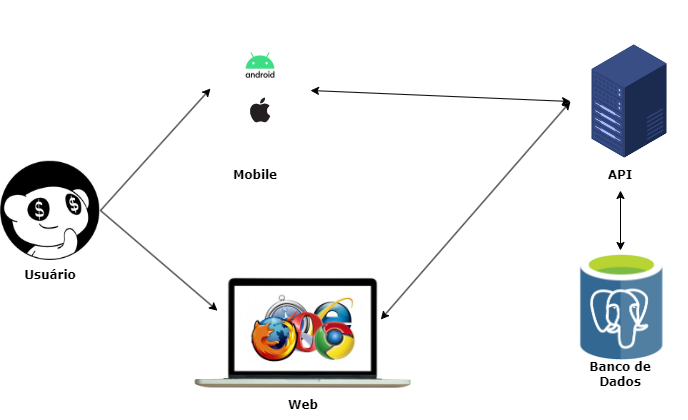
\includegraphics[width = 130mm]{fig/Arquitetura.drawio.png}}{O Autor (2024)}{arquitetura}{nota(s)}{legenda(s)}

Para o desenvolvimento da parte mobile optou-se por utilizar o Flutter, um framework robusto para o desenvolvimento de aplicativos móveis criado pela Google. Para a comunicação com o banco de dados optou-se por construir uma API utilizando o Spring, framework de desenvolvimento de aplicações Java. E por fim o banco de dados escolhido foi o PostgreSQL. Abaixo tais tecnologias são apresentadas com mais detalhes.

\subsection{DART \& FLUTTER}
Dart é uma linguagem orientada a objetos com foco em performance e produtividade, especialmente no desenvolvimento de aplicações web e móveis \cite{dart}.

Flutter é um framework de desenvolvimento de aplicativos móveis criado pelo Google. Utiliza a linguagem de programação Dart e permite a criação de interfaces de usuário altamente interativas e responsivas \cite{flutter}.

\subsection{JAVA \& SPRING}
Java é uma linguagem de programação amplamente utilizada em desenvolvimento de software, especialmente em aplicações empresariais. Java é conhecido pela sua portabilidade, robustez e segurança, sendo a base para diversos frameworks e tecnologias como Spring, Hibernate e Java EE \cite{java}.

Spring é um framework de desenvolvimento de aplicações Java, utilizado para criar APIs RESTful e aplicações empresariais escaláveis. É amplamente conhecido pela sua facilidade de configuração e integração, além de oferecer suporte a diversas tecnologias Java como Spring Boot e Spring MVC \cite{spring}.

\subsection{POSTGRESQL}
Sistema de gerenciamento de banco de dados relacional de código aberto. É conhecido pela sua confiabilidade, escalabilidade e suporte a recursos avançados como transações ACID e extensões customizadas \cite{postgresql}.

\subsection{HARDWARE}
O hardware utilizado para o desenvolvimento do sistema é um computador somente, com processador AMD Ryzen 5 3600, 16GB de memória RAM, AMD Radeon RX 570 e 1 HD de 1TB de armazenamento.

O sistema operacional utilizado foi o Linux Ubuntu 22. A escolha do Linux como ambiente de desenvolvimento para o aplicativo foi fundamentada em diversos aspectos que favorecem a eficiência, segurança e flexibilidade durante o processo de desenvolvimento. 

Os códigos foram escritos utilizando o editor de texto VSCode, que é amplamente conhecido por sua interface intuitiva e leve, oferecendo uma experiência de desenvolvimento fluida e sem interrupções. Sua ampla gama de extensões e plugins disponíveis no Marketplace permite integrar facilmente com todas as tecnolgias descritas anteriormente.

% Desenho do Processo Macro
% ----------------------------------------------------------
\chapter{Desenho do Processo Macro} \label{cha:desenhomacro}
Neste capítulo são apresentados os diagramas de atividades das principais funcionalidades que serão implementados no aplicativo.

%DUVIDA: MTO PEQUENO SÓ ATIVIDADES?

A atividade "Buscar Produto", diagramada na figura \autoref{fig:atividade_comparar}, na qual o usuário insere um termo de pesquisa para encontrar produtos de interesse. Em seguida, o sistema executa a ação de "Pesquisar Produto", onde são consultadas as lojas cadastradas para encontrar produtos que correspondam ao termo de pesquisa. Após a pesquisa, o sistema verifica se foram encontrados produtos. Se sim, o fluxo segue para a atividade "Comparar Preços", na qual os preços dos produtos encontrados são coletados e comparados entre as diferentes lojas ou fontes disponíveis. Durante essa comparação, o sistema identifica o melhor preço para cada produto.

Ao final da atividade de comparar preços, o sistema pode exibir os resultados da comparação ao usuário, mostrando os produtos encontrados, seus preços em diferentes lojas e destacando o melhor preço disponível. Isso ajuda o usuário a tomar uma decisão informada sobre qual produto comprar com base no preço mais atrativo.

A atividade de visualizar ou alterar sugestões de preços, diagramada na figura \autoref{fig:atividade_sugestoes}, tem início na etapa de visualização de detalhes do produto. Caso o produto já tenha um preço cadastrado o usuário pode avaliar a sugestão ou inserir outra. Essa atualização é fundamental para garantir que os usuários recebam informações precisas e atualizadas sobre os preços dos produtos que estão monitorando ou pesquisando.

\imagem{DIAGRAMA DE ATIVIDADES COMPARAR PREÇOS}{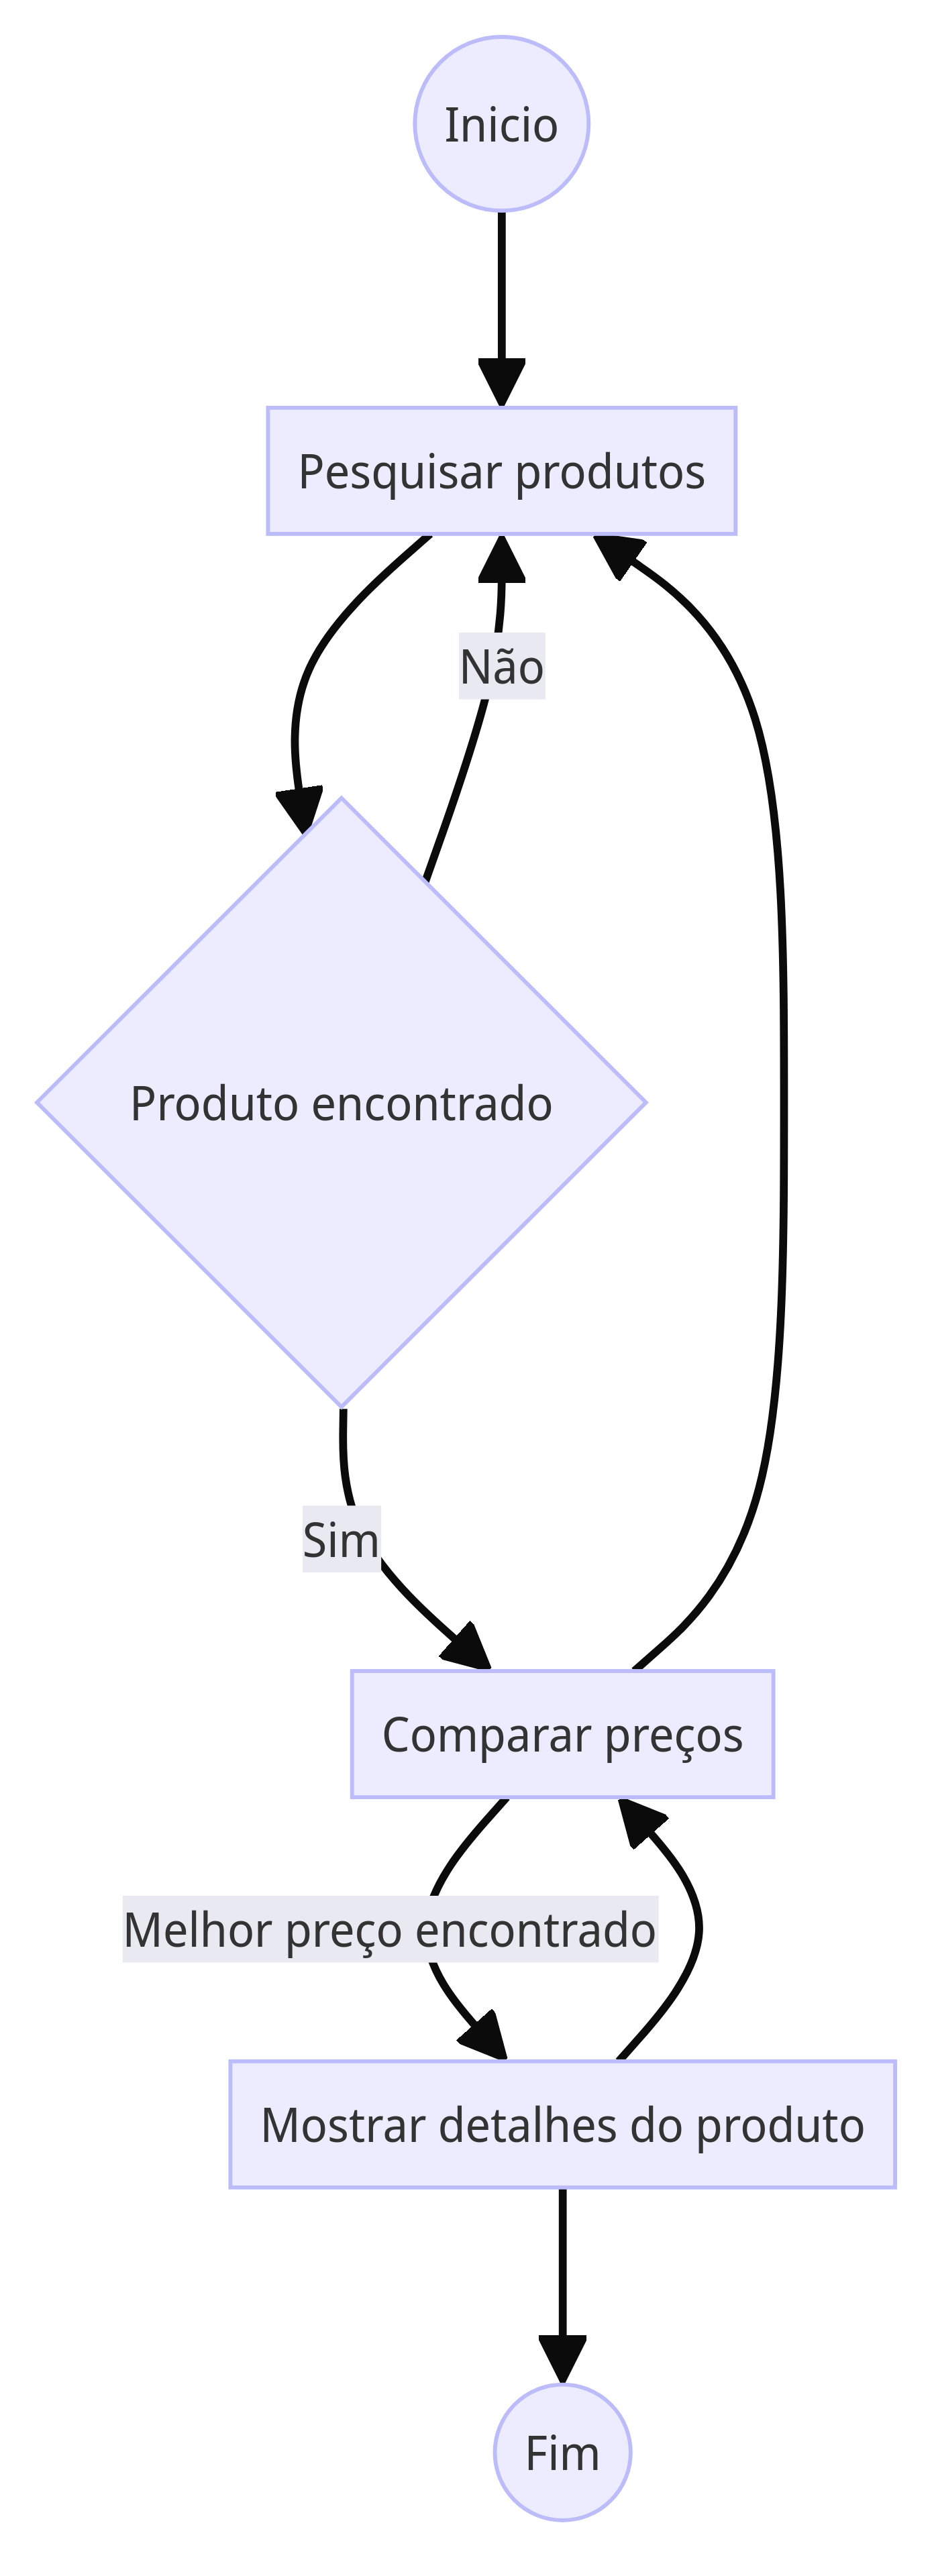
\includegraphics[width = 60mm]{fig/atividade/atividade1.png}}{O Autor (2024)}{fig:atividade_comparar}{nota(s)}{legenda(s)}

\imagem{DIAGRAMA DE ATIVIDADES SUGESTÕES PREÇO}{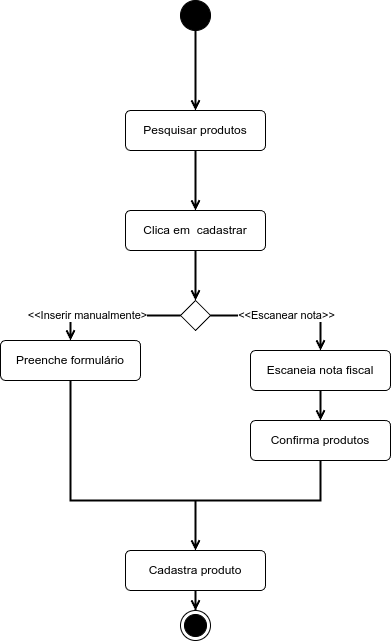
\includegraphics[width = 120mm]{fig/atividade/atividade2.png}}{O Autor (2024)}{fig:atividade_sugestoes}{nota(s)}{legenda(s)}

% Diagrama de Casos de Uso
% ----------------------------------------------------------
\chapter{Diagrama de Casos de Uso} \label{cha:diagramacasouso}

Neste capítulo é apresentado o diagrama de casos de uso do aplicativo proposto, onde é possível visualizar de forma clara e organizada as principais funcionalidades e interações entre os atores (Usuário e Lojista) e o sistema. O diagrama de casos de uso oferece uma visão geral das ações que podem ser realizadas pelos usuários do aplicativo, como buscar produtos, comparar preços, cadastrar produtos, entre outras.

%DUVIDA: cada caso de uso = tela = historia?

\imagem{DIAGRAMA DE CASOS DE USO}{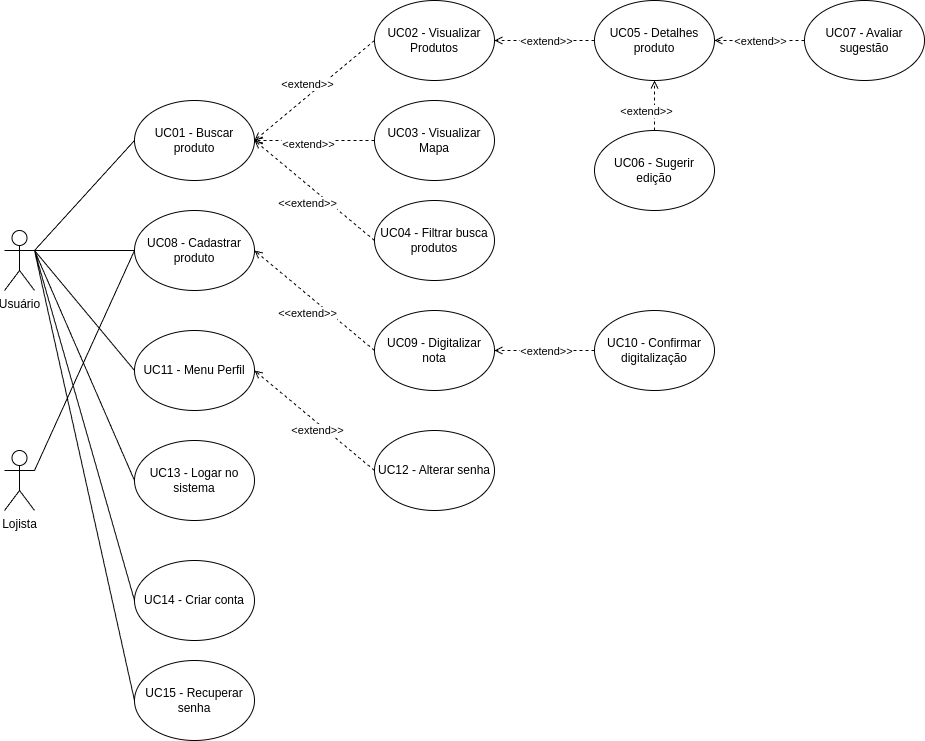
\includegraphics[width = 170mm]{fig/usecase.drawio.png}}{O Autor (2024)}{usecase}{nota(s)}{legenda(s)}

% Histórias de Usuário
% ----------------------------------------------------------
\chapter{Histórias de Usuário} \label{cha:historiasUsuário}

Neste capítulo serão apresentadas as histórias de usuários definidas para o desenvolvimento deste software. As histórias são descritas de forma detalhada e contextualizada as necessidades, objetivos e requisitos específicos dos usuários em relação ao sistema. Cada história de usuário é uma narrativa curta que descreve uma funcionalidade. As histórias de usuário são uma ferramenta importante para o desenvolvimento ágil de software, pois permitem uma compreensão clara das expectativas dos usuários e fornecem direcionamento para o desenvolvimento incremental e iterativo do aplicativo.

\section{Buscar produto}%%%%%%%%%%%%%%%%%%%%%%%%%%%%%%%%%%%%%

\newcounter{numhistoria}
\setcounter{numhistoria}{1}
\newcommand{\nhist}{%
  \padzeroes[2]{\decimal{numhistoria}}%
  \stepcounter{numhistoria}%
}

%\begin{quadro}[hbt!]
%\centering
\begin{tabular}{|ll|}
\hline
\multicolumn{2}{|c|}{\textbf{UC\nhist - \currentname}}    \\ \hline
\multicolumn{1}{|l|}{\textbf{Sendo}}     & um usuário \\ \hline
\multicolumn{1}{|l|}{\textbf{Quero}}     & buscar um produto \\ \hline
\multicolumn{1}{|l|}{\textbf{Para}}      & encontrar oque tenha melhor preço e localização \\ \hline
\multicolumn{1}{|l|}{\textbf{Protótipo}} & 
\begin{minipage}{0.48\textwidth} 
\begin{figure}[H]
\caption{\label{fig:label} TELA INICIAL}
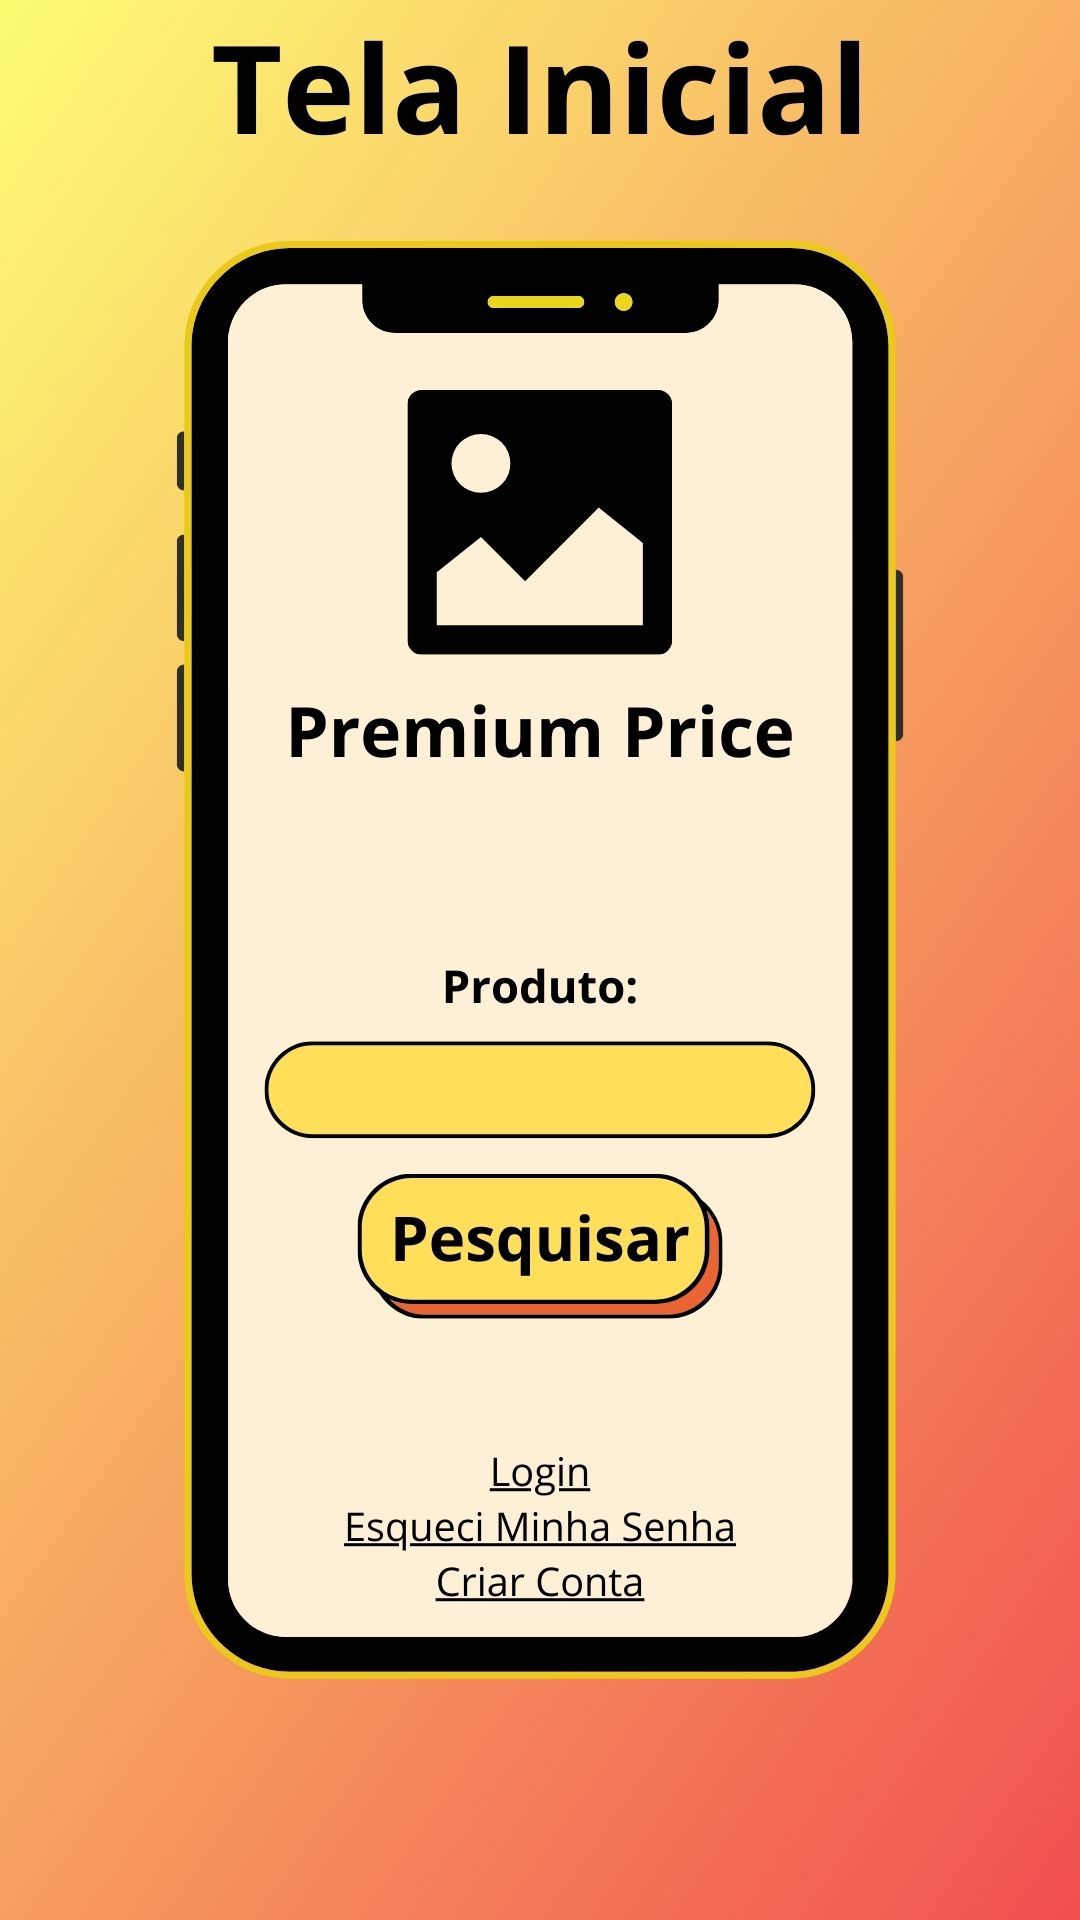
\includegraphics[width=\textwidth]{fig/telas/t_inicial.jpg}
\footnotesize \centering
\par FONTE: O Autor (2024)
\end{figure}
\end{minipage} \\ \hline
\end{tabular}
%\end{quadro}



\subsection*{\textbf{CRITÉRIOS DE ACEITAÇÃO}}

\begin{enumerate}[leftmargin=2cm]
    \item Deve permitir inserir o nome do produto.
    \item Deve definir a localização do usuário por GPS.
    \item Deve permitir que o usuário logue no sistema.
    \item Deve permitir que o usuário recupere a senha.
    \item Deve permitir que o usuário se cadastre.
    \item Deve buscar os produtos por nome.
\end{enumerate}

\subsection*{\textbf{CRITÉRIOS DE ACEITAÇÃO - DETALHAMENTO}}

\begin{tabularx}{0.9\textwidth}{|l|X|}
\multicolumn{2}{@{}l}{\textbf{1. Deve permitir inserir o nome do produto.}} \\ \hline
\textbf{Dado que} & Usuário está na tela de pesquisa. \\ \hline
\textbf{Quanto} & Usuário clica no campo "Produto". \\ \hline
\textbf{Então} & Sistema permite a inserção do nome do produto. (R1)\\ \hline
\end{tabularx}

\begin{tabularx}{0.9\textwidth}{|l|X|}
\multicolumn{2}{@{}l}{\textbf{2. Deve definir a localização do usuário por GPS.}} \\ \hline
\textbf{Dado que} & Usuário está na tela inicial.\\ \hline
\textbf{Quanto} & Usuário realiza qualquer requisição. \\ \hline
\textbf{Então} & Sistema salva a localização do usuário através do ip. \\ \hline
\end{tabularx}

\begin{tabularx}{0.9\textwidth}{|l|X|}
\multicolumn{2}{@{}l}{\textbf{3. Deve permitir que o usuário logue no sistema.}} \\ \hline
\textbf{Dado que} & Usuário está na tela de pesquisa. \\ \hline
\textbf{Quanto} & Usuário clica no botão "Login". \\ \hline
\textbf{Então} & Sistema redireciona para a tela de login. \\ \hline
\end{tabularx}

\begin{tabularx}{0.9\textwidth}{|l|X|}
\multicolumn{2}{@{}l}{\textbf{4. Deve permitir que o usuário recupere a senha.}} \\ \hline
\textbf{Dado que} & Usuário está na tela de pesquisa. \\ \hline
\textbf{Quanto} & Usuário lica no botão "Esqueci minha senha". \\ \hline
\textbf{Então} & Sistema redireciona para a tela. \\ \hline
\end{tabularx}

\begin{tabularx}{0.9\textwidth}{|l|X|}
\multicolumn{2}{@{}l}{\textbf{5. Deve permitir que o usuário se cadastre.}} \\ \hline
\textbf{Dado que} & Usuário está na tela de pesquisa. \\ \hline
\textbf{Quanto} &  Usuário clica no botão "Criar conta". \\ \hline
\textbf{Então} & Sistema redireciona para a tela de cadastro. \\ \hline
\end{tabularx}

\begin{tabularx}{0.9\textwidth}{|l|X|}
\multicolumn{2}{@{}l}{\textbf{6. Deve buscar os produtos por nome.}} \\ \hline
\textbf{Dado que} & Usuário inseriu o nome de um produto. (R1) \\ \hline
\textbf{Quanto} & Usuário clica em "Pesquisar". \\ \hline
\textbf{Então} & Sistema redireciona para a tela com os produtos buscados. \\ \hline
\end{tabularx}

\subsection*{\textbf{REGRAS DE NEGÓCIO DA HISTÓRIA}}

\begin{itemize}
    \item[] R1 - Tamanho máximo do texto 256 caracteres.
\end{itemize}

\section{Visualizar produtos}%%%%%%%%%%%%%%%%%%%%%%%%%%%%%%%%%%%%%

\begin{tabular}{|ll|}
\hline
\multicolumn{2}{|c|}{\textbf{UC\nhist - \currentname}}    \\ \hline
\multicolumn{1}{|l|}{\textbf{Sendo}}     & um usuário \\ \hline
\multicolumn{1}{|l|}{\textbf{Quero}}     & visualizar os produtos buscados\\ \hline
\multicolumn{1}{|l|}{\textbf{Para}}      & selecionar oque tenha melhor preço e localização \\ \hline
\multicolumn{1}{|l|}{\textbf{Protótipo}} & 
\begin{minipage}{0.48\textwidth} 
\begin{figure}[H]
\caption{\label{fig:label} TELA VISUALIZAR PRODUTOS}
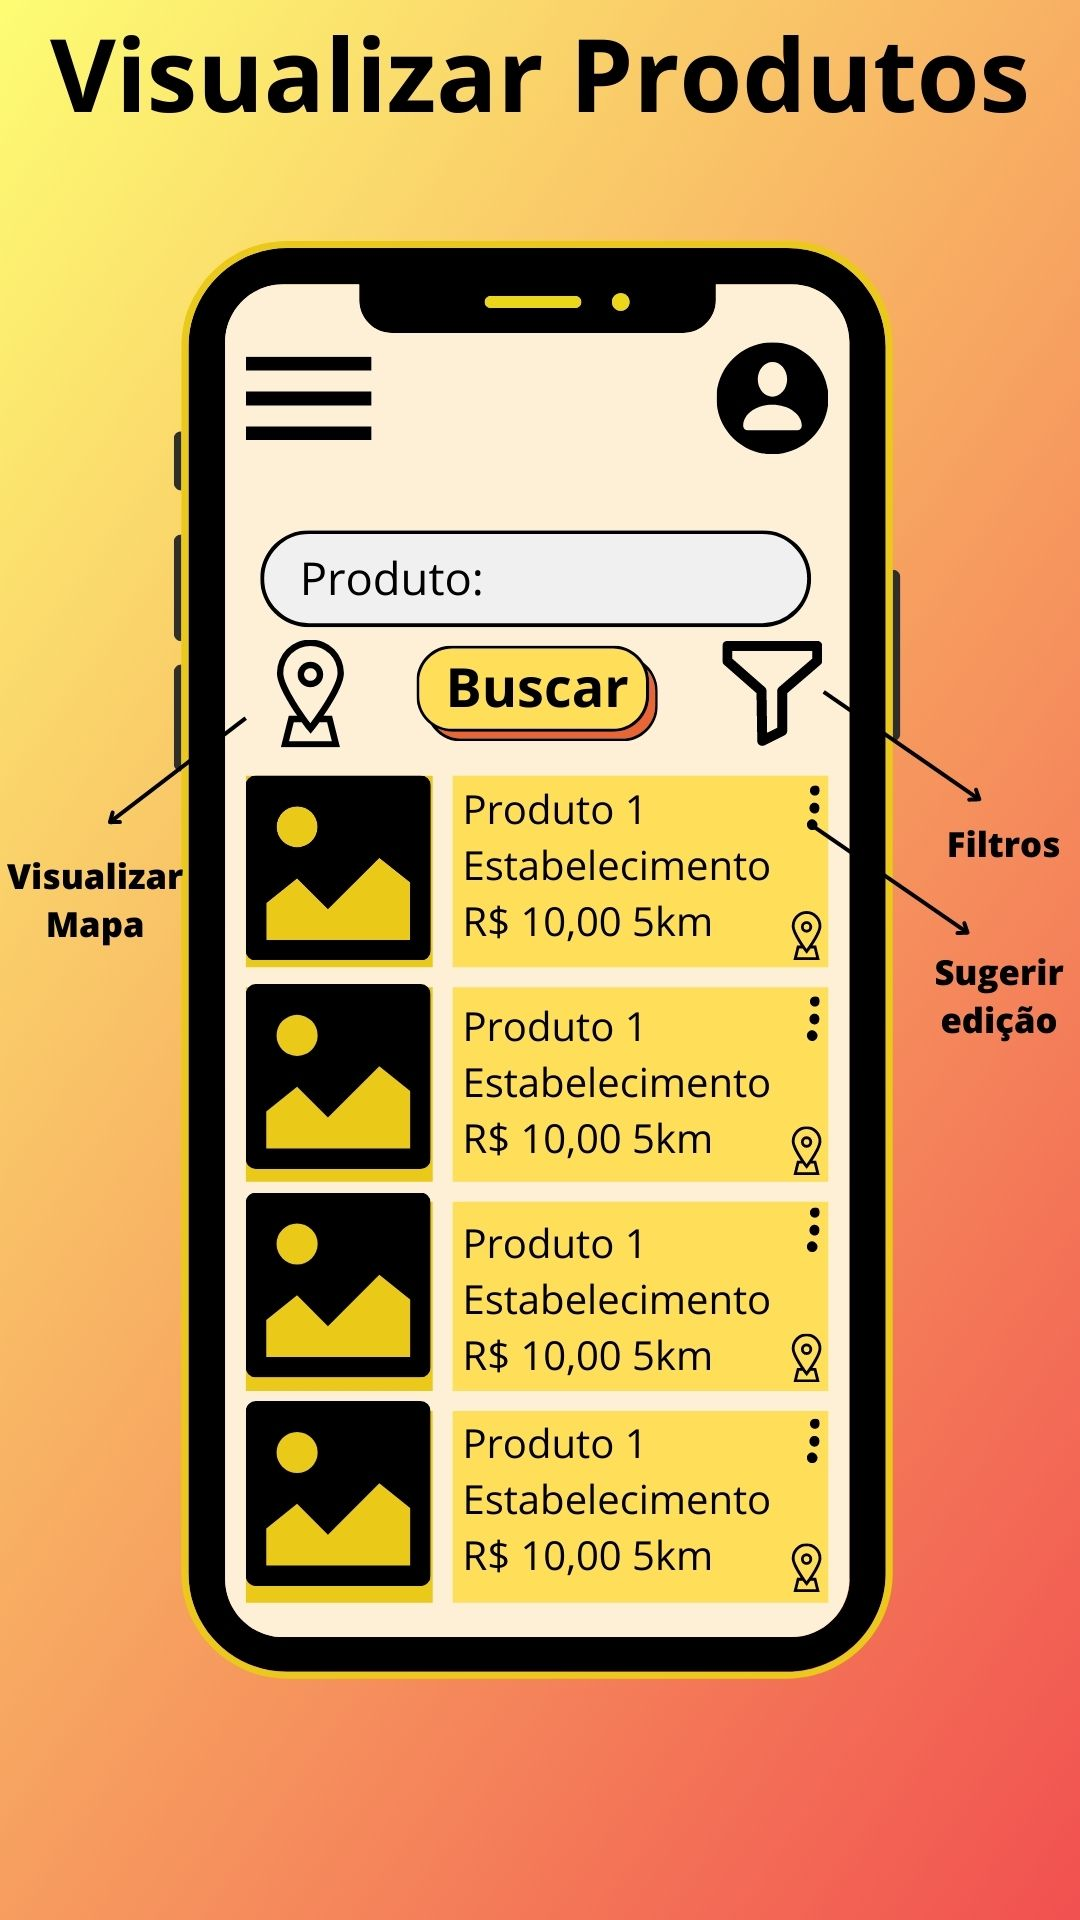
\includegraphics[width=\textwidth]{fig/telas/t_listarprod.jpg}
\footnotesize \centering
\par FONTE: O Autor (2024)
\end{figure}
\end{minipage}
 \\ \hline
\end{tabular}

\subsection*{\textbf{CRITÉRIOS DE ACEITAÇÃO}}

\begin{enumerate}[leftmargin=2cm]
    \item Deve listar os produtos buscados.
    \item Deve permitir fazer uma nova busca.
    \item Deve permitir selecionar um produto na lista para mostrar mais detalhes.
    \item Deve permitir visualizar os produtos por mapa.
    \item Deve permitir filtrar a busca.
\end{enumerate}

\subsection*{\textbf{CRITÉRIOS DE ACEITAÇÃO - DETALHAMENTO}}
%\textbf{Critério de contexto} (Válido como premissa para todos os critérios):

%\begin{tabular}{@{}l l }
% \textbf{Dado que} & blabla \\ 
% \textbf{E} & blabla
%\end{tabular}

\begin{tabularx}{0.9\textwidth}{|l|X|}
\multicolumn{2}{@{}l}{\textbf{1. Deve listar os produtos buscados.}} \\ \hline
\textbf{Dado que} & Usuário pesquisou um produto valido. (R1)  \\ \hline
\textbf{Quanto} & Sistema carrega a tela. \\ \hline
\textbf{Então} & Sistema apresenta a lista dos produtos encontrados.  \\ \hline
\end{tabularx}

\begin{tabularx}{0.9\textwidth}{|l|X|}
\multicolumn{2}{@{}l}{\textbf{2. Deve permitir fazer uma nova busca.}} \\ \hline
\textbf{Dado que} & Usuário inseriu o nome de um produto. (R2) \\ \hline
\textbf{Quanto} & Usuário clica em "Buscar". \\ \hline
\textbf{Então} & Sistema carrega nova lista. \\ \hline
\end{tabularx}

\begin{tabularx}{0.9\textwidth}{|l|X|}
\multicolumn{2}{@{}l}{\textbf{\makecell[l]{3. Deve permitir selecionar um produto na lista para mostrar mais \\detalhes.}}} \\ \\
\hline \textbf{Dado que} & Sistema carregou ao menos 1 produto. (R1) \\ \hline
\textbf{Quanto} & Usuário clica em um produto. \\ \hline
\textbf{Então} & Sistema redireciona para tela de detalhe. \\ \hline
\end{tabularx}

\begin{tabularx}{0.9\textwidth}{|l|X|}
\multicolumn{2}{@{}l}{\textbf{4. Deve permitir visualizar os produtos por mapa.}} \\ \hline
\textbf{Dado que} & Sistema carregou ao menos 1 produto. (R1) \\ \hline
\textbf{Quanto} & Usuário clica no ícone de mapa de um produto. \\ \hline
\textbf{Então} & Sistema apresenta a visualização por mapa. \\ \hline
\end{tabularx}

\begin{tabularx}{0.9\textwidth}{|l|X|}
\multicolumn{2}{@{}l}{\textbf{5. Deve permitir filtrar a busca.}} \\ \hline
\textbf{Dado que} & Usuário está na tela de listagem. \\ \hline
\textbf{Quanto} & Usuário clica no ícone de filtro. \\ \hline
\textbf{Então} & Sistema apresenta as opções de filtragem. \\ \hline
\end{tabularx}

\subsection*{\textbf{REGRAS DE NEGÓCIO DA HISTÓRIA}}

\begin{itemize}
    \item[] R1 - Produto cadastrado no banco de dados.
    \item[] R2 - Tamanho máximo do texto 256 caracteres.
\end{itemize}

\section{Visualizar mapa}%%%%%%%%%%%%%%%%%%%%%%%%%%%%%%%%%%%%%

\begin{tabular}{|ll|}
\hline
\multicolumn{2}{|c|}{\textbf{UC\nhist - \currentname}}    \\ \hline
\multicolumn{1}{|l|}{\textbf{Sendo}}     & um usuário \\ \hline
\multicolumn{1}{|l|}{\textbf{Quero}}     & visualizar os produtos buscados no mapa\\ \hline
\multicolumn{1}{|l|}{\textbf{Para}}      & verificar no mapa a localização do estabelecimento\\ \hline
\multicolumn{1}{|l|}{\textbf{Protótipo}} & 
\begin{minipage}{0.48\textwidth} 
\begin{figure}[H]
\caption{\label{fig:label} TELA MAPA}
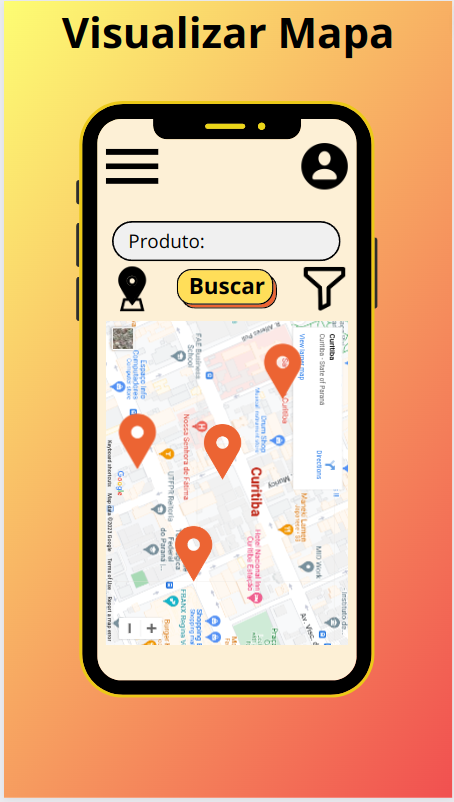
\includegraphics[width=\textwidth]{fig/telas/t_mapa.png}
\footnotesize \centering
\par FONTE: O Autor (2024)
\end{figure}
\end{minipage}
 \\ \hline
\end{tabular}

\subsection*{\textbf{CRITÉRIOS DE ACEITAÇÃO}}

\begin{enumerate}[leftmargin=2cm]
    \item Deve definir a localização do usuário por GPS.
    \item Deve mostrar os produtos buscados em suas respectivas localizações no mapa.
    \item Deve permitir fazer uma nova busca.
    \item Deve permitir selecionar uma localização no mapa para mostrar mais detalhes.
\end{enumerate}

\subsection*{\textbf{CRITÉRIOS DE ACEITAÇÃO - DETALHAMENTO}}


\begin{tabularx}{0.9\textwidth}{|l|X|}
\multicolumn{2}{@{}l}{\textbf{1. Deve definir a localização do usuário por GPS.}} \\ \hline
\textbf{Dado que} & Usuário selecionou um produto. \\ \hline
\textbf{Quanto} & Sistema apresenta visualização por mapa. \\ \hline
\textbf{Então} & Sistema salva localização do usuário por ip. \\ \hline
\end{tabularx}

\begin{tabularx}{0.9\textwidth}{|l|X|}
\multicolumn{2}{@{}l}{\textbf{\makecell[l]{2. Deve mostrar os produtos buscados em suas respectivas \\localizações no mapa.}}} \\ \hline
\textbf{Dado que} & Usuário selecionou um produto. \\ \hline
\textbf{Quanto} & Usuário está na tela do mapa. \\ \hline
\textbf{Então} & Sistema mostra os produtos em seus respectivos locais no mapa. \\ \hline
\end{tabularx}

\begin{tabularx}{0.9\textwidth}{|l|X|}
\multicolumn{2}{@{}l}{\textbf{3. Deve permitir fazer uma nova busca}} \\ \hline
\textbf{Dado que} & Usuário inseriu o nome de um produto. (R2)\\ \hline
\textbf{Quanto} & Usuário clica em "Buscar". \\ \hline
\textbf{Então} & Sistema redireciona para tela de listagem. \\ \hline
\end{tabularx}

\begin{tabularx}{0.9\textwidth}{|l|X|}
\multicolumn{2}{@{}l}{\textbf{\makecell[l]{4. Deve permitir selecionar uma localização no mapa para mostrar \\mais detalhes.}}} \\ \hline
\textbf{Dado que} & Sistema encontrou 1 produto. (R1) \\ \hline
\textbf{Quanto} & Usuário seleciona um produto no mapa. \\ \hline
\textbf{Então} & Sistema redireciona para tela de detalhe. \\ \hline
\end{tabularx}

\subsection*{\textbf{REGRAS DE NEGÓCIO DA HISTÓRIA}}

\begin{itemize}
    \item[] R1 - Produto cadastrado no banco de dados.
    \item[] R2 - Tamanho máximo do texto 256 caracteres.
\end{itemize}


\section{Filtrar busca produtos}%%%%%%%%%%%%%%%%%%%%%%%%%%%%%%%%%%%%%

\begin{tabular}{|ll|}
\hline
\multicolumn{2}{|c|}{\textbf{UC\nhist - \currentname}}    \\ \hline
\multicolumn{1}{|l|}{\textbf{Sendo}}     & um usuário \\ \hline
\multicolumn{1}{|l|}{\textbf{Quero}}     & filtrar a minha busca\\ \hline
\multicolumn{1}{|l|}{\textbf{Para}}      & encontrar um produto especificando os parâmetros da busca\\ \hline
\multicolumn{1}{|l|}{\textbf{Protótipo}} & 
\begin{minipage}{0.48\textwidth} 
\begin{figure}[H]
\caption{\label{fig:label} TELA FILTRAR BUSCA}
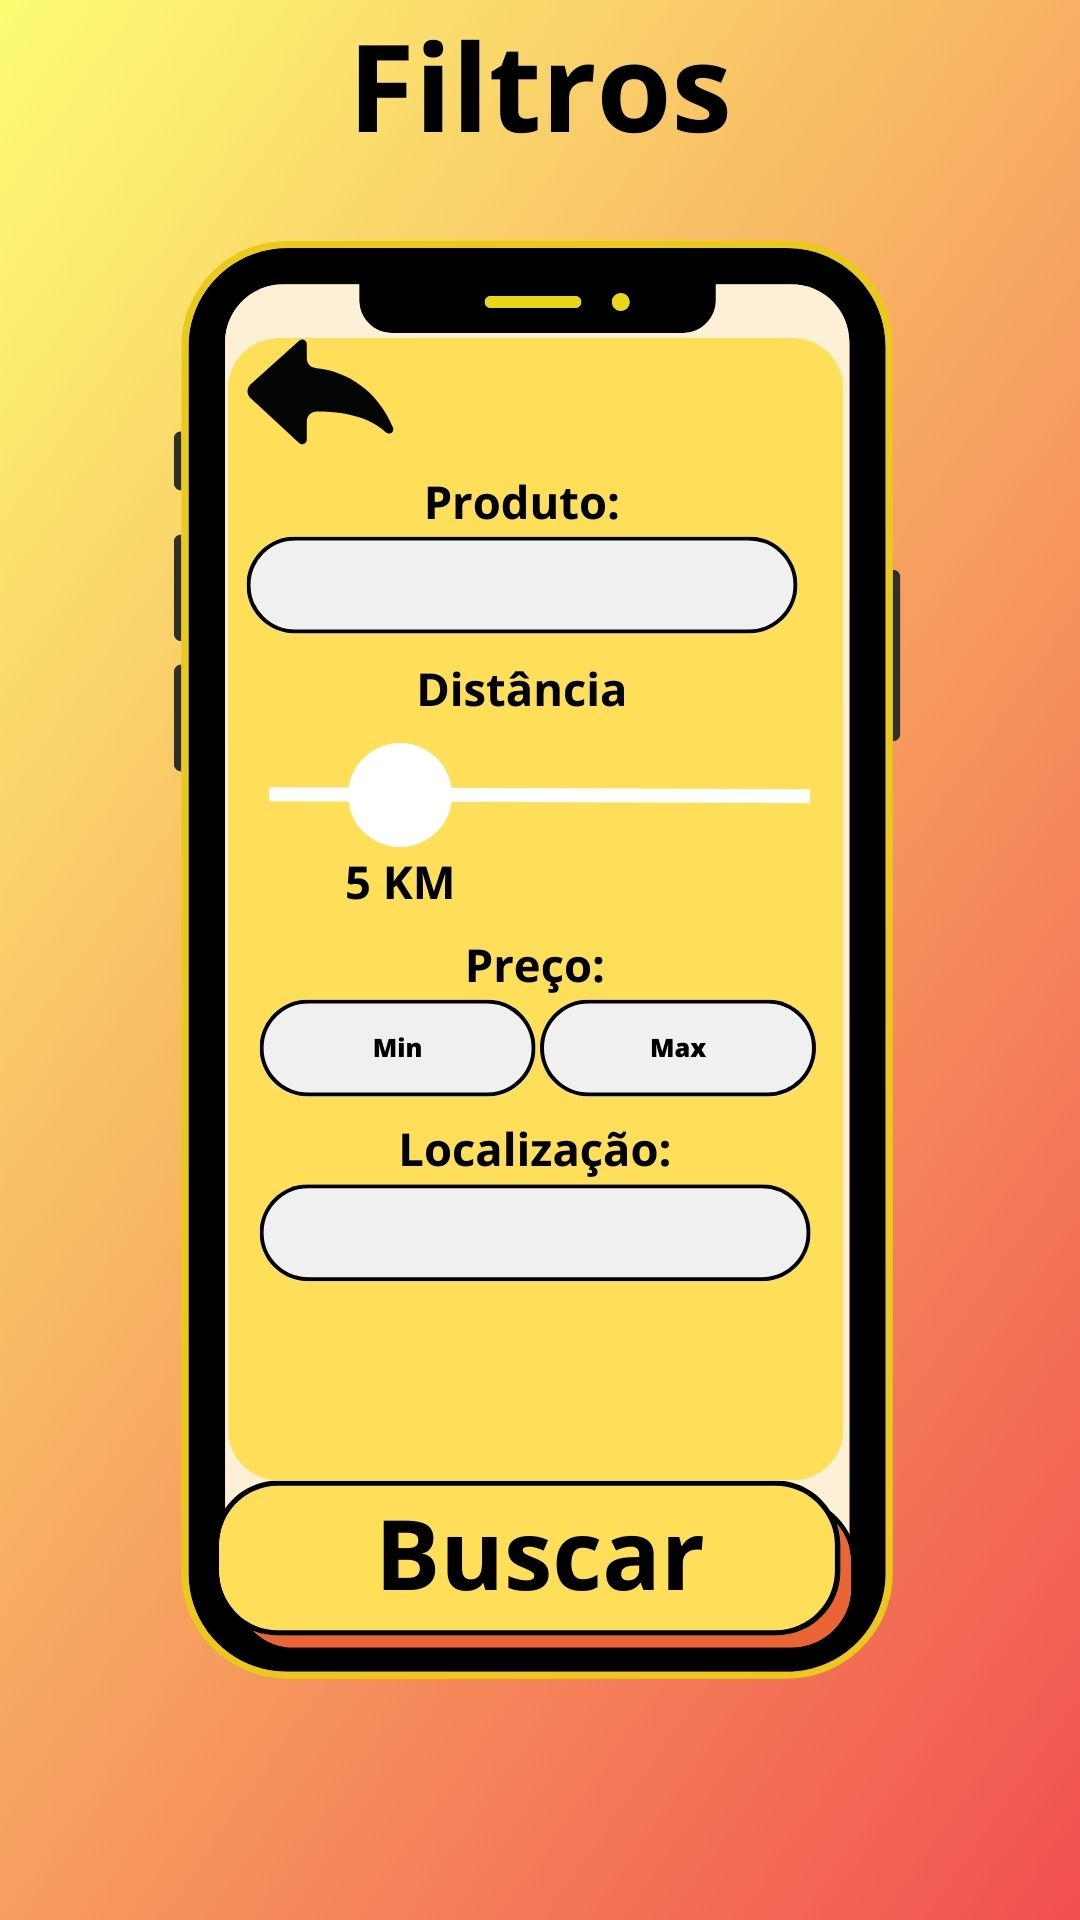
\includegraphics[width=\textwidth]{fig/telas/t_filtros.jpg}
\footnotesize \centering
\par FONTE: O Autor (2024)
\end{figure}
\end{minipage}
 \\ \hline
\end{tabular}

\subsection*{\textbf{CRITÉRIOS DE ACEITAÇÃO}}

\begin{enumerate}[leftmargin=2cm]
    \item Deve permitir inserir o nome do produto.
    \item Deve permitir especificar a distância máxima.
    \item Deve permitir especificar o preço mínimo e máximo.
    \item Deve permitir especificar a localização do produto.
\end{enumerate}

\subsection*{\textbf{CRITÉRIOS DE ACEITAÇÃO - DETALHAMENTO}}


\begin{tabularx}{0.9\textwidth}{|l|X|}
\multicolumn{2}{@{}l}{\textbf{1. Deve permitir inserir o nome do produto.}} \\ \hline
\textbf{Dado que} & Usuário clicou no ícone de filtro. \\ \hline
\textbf{Quanto} & Usuário clica no campo "Produto". \\ \hline
\textbf{Então} & Sistema permite inserir nome de um produto. (R1)\\ \hline
\end{tabularx}

\begin{tabularx}{0.9\textwidth}{|l|X|}
\multicolumn{2}{@{}l}{\textbf{2. Deve permitir especificar a distância máxima.}} \\ \hline
\textbf{Dado que} & Usuário clicou no ícone de filtro. \\ \hline
\textbf{Quanto} & Usuário clica no campo "Distância". \\ \hline
\textbf{Então} & Sistema permite inserir distância. (R2) \\ \hline
\end{tabularx}

\begin{tabularx}{0.9\textwidth}{|l|X|}
\multicolumn{2}{@{}l}{\textbf{3. Deve permitir especificar o preço mínimo e máximo.}} \\ \hline
\textbf{Dado que} & Usuário clicou no ícone de filtro. \\ \hline
\textbf{Quanto} & Usuário clica no campo "Preço". \\ \hline
\textbf{Então} & Sistema permite inserir preço mínimo e máximo. (R3) \\ \hline
\end{tabularx}

\begin{tabularx}{0.9\textwidth}{|l|X|}
\multicolumn{2}{@{}l}{\textbf{4. Deve permitir especificar a localização do produto.}} \\ \hline
\textbf{Dado que} & Usuário clicou no ícone de filtro  \\ \hline
\textbf{Quanto} & Usuário clica no campo "Localização". \\ \hline
\textbf{Então} & Sistema permite inserir localização. (R4) \\ \hline
\end{tabularx}

\subsection*{\textbf{REGRAS DE NEGÓCIO DA HISTÓRIA}}

\begin{itemize}
    \item[] R1 - Tamanho máximo do texto 256 caracteres.
    \item[] R2 - Distância mínima 1km, distância máxima 15km.
    \item[] R3 - Preço mínimo 0, preço máximo 999,999.
    \item[] R4 - CEP válido ou localização no mapa.
\end{itemize}



\section{Detalhes produto}%%%%%%%%%%%%%%%%%%%%%%%%%%%%%%%%%%%%%

\begin{tabular}{|ll|}
\hline
\multicolumn{2}{|c|}{\textbf{UC\nhist - \currentname}}    \\ \hline
\multicolumn{1}{|l|}{\textbf{Sendo}}     & um usuário \\ \hline
\multicolumn{1}{|l|}{\textbf{Quero}}     & visualizar os detalhes do produto\\ \hline
\multicolumn{1}{|l|}{\textbf{Para}}      & analisar a localização e preço do produto\\ \hline
\multicolumn{1}{|l|}{\textbf{Protótipo}} & 
\begin{minipage}{0.48\textwidth} 
\begin{figure}[H]
\caption{\label{fig:label} TELA DETALHES PRODUTO}
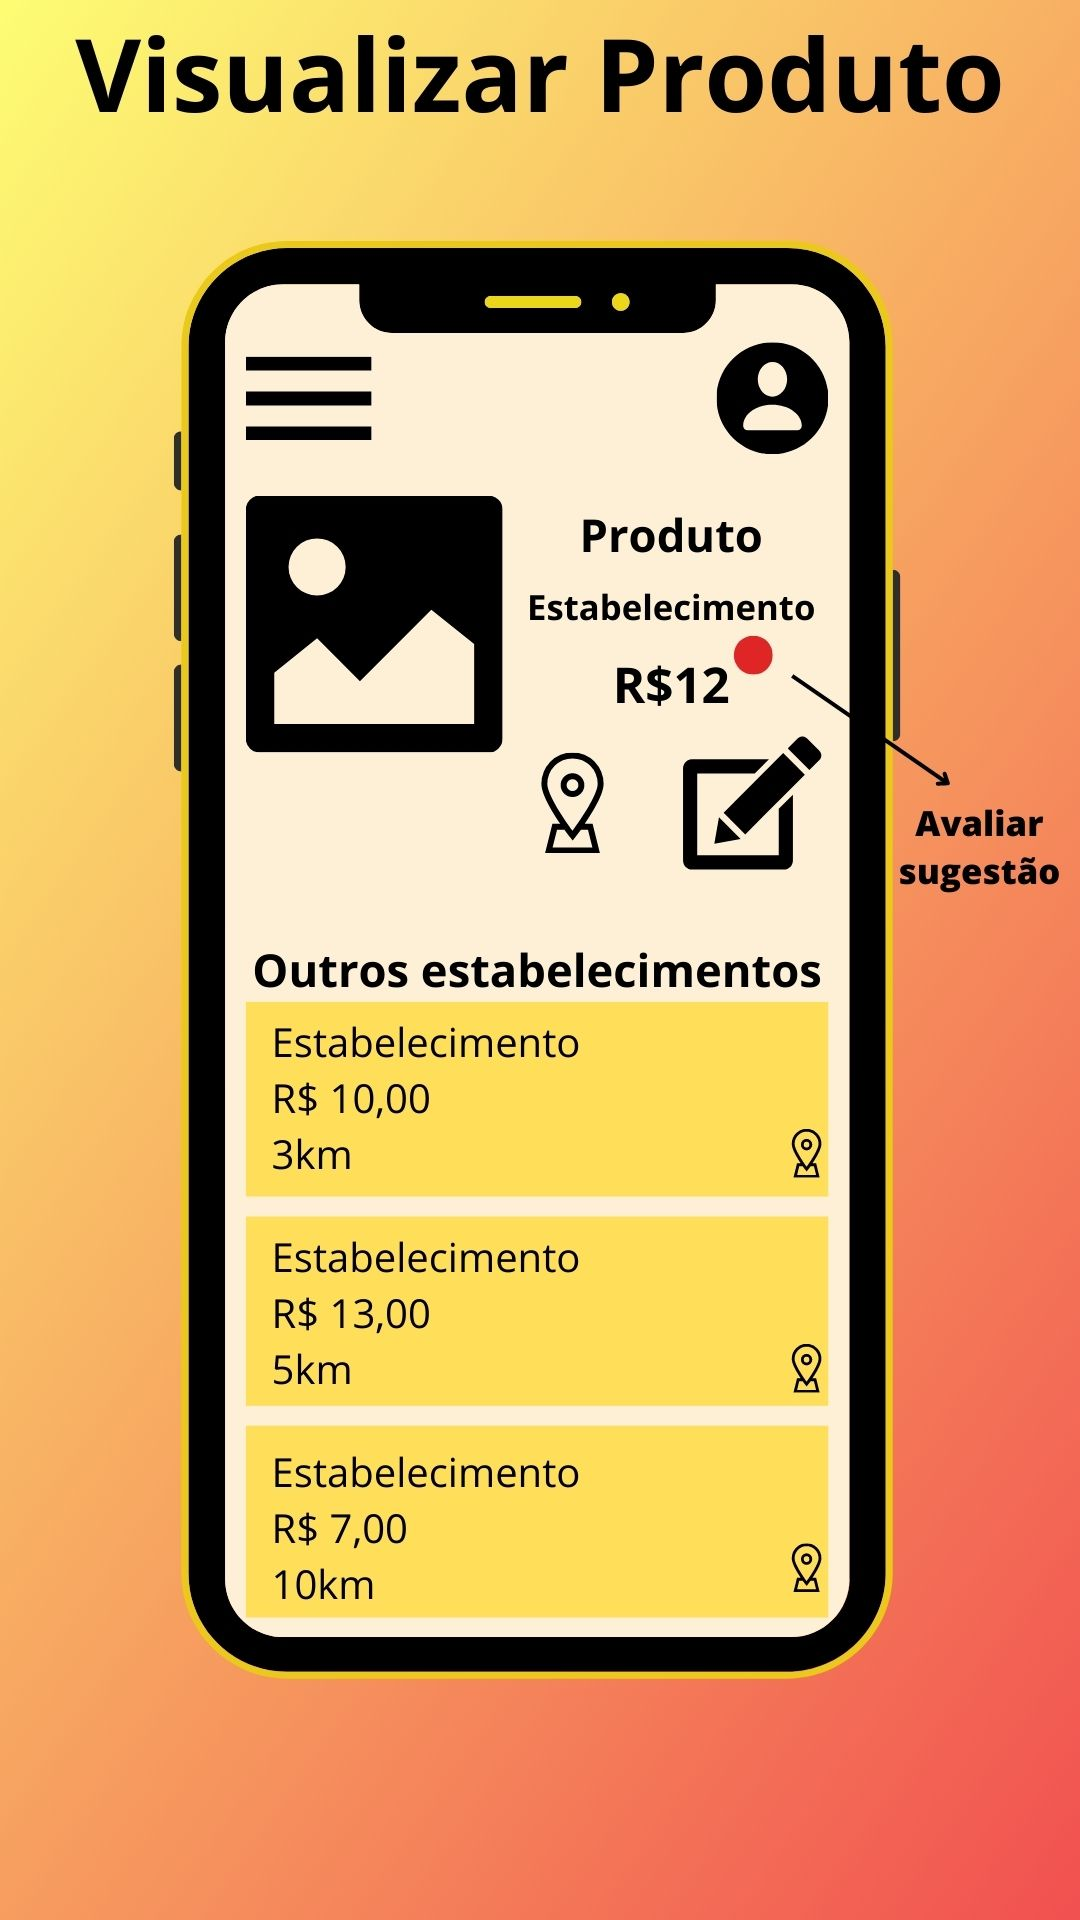
\includegraphics[width=\textwidth]{fig/telas/t_produto.jpg}
\footnotesize \centering
\par FONTE: O Autor (2024)
\end{figure}
\end{minipage}
 \\ \hline
\end{tabular}

\subsection*{\textbf{CRITÉRIOS DE ACEITAÇÃO}}

\begin{enumerate}[leftmargin=2cm]
    \item Deve mostrar as informações do produto como: foto, nome, estabelecimento, preço e localização.
    \item Deve mostrar outros estabelecimentos com o mesmo produto ordenado por distância.
    \item Deve permitir mostrar o estabelecimento no mapa.
    \item Deve permitir sugerir um novo preço para o produto no estabelecimento.
\end{enumerate}

\subsection*{\textbf{CRITÉRIOS DE ACEITAÇÃO - DETALHAMENTO}}
\textbf{Critério de contexto} (Válido como premissa para todos os critérios):

\begin{tabularx}{0.9\textwidth}{@{}l X }
 \textbf{Dado que} & Sistema buscou ao menos 1 produto. \\ 
 \textbf{E} & Usuário clicou em 1 produto.
\end{tabularx}


\begin{tabularx}{0.9\textwidth}{|l|X|}
\multicolumn{2}{@{}l}{\textbf{\makecell[l]{1. Deve mostrar as informações do produto como: foto, nome, \\estabelecimento, preço e localização.}}} \\ \hline
\textbf{Dado que} & Usuário está na tela de detalhe. \\ \hline
\textbf{Quanto} & Sistema carrega informações do produto. \\ \hline
\textbf{Então} & Sistema apresenta informações do produto. \\ \hline
\end{tabularx}

\begin{tabularx}{0.9\textwidth}{|l|X|}
\multicolumn{2}{@{}l}{\textbf{\makecell[l]{2. Deve mostrar outros estabelecimentos com o mesmo produto \\ordenado por distância.}}} \\ \hline
\textbf{Dado que} & Usuário está na tela de detalhe. \\ \hline
\textbf{Quanto} & Sistema carrega informações do produto. \\ \hline
\textbf{Então} & Sistema apresenta outras lojas com o mesmo produto. \\ \hline
\end{tabularx}

\begin{tabularx}{0.9\textwidth}{|l|X|}
\multicolumn{2}{@{}l}{\textbf{3. Deve permitir mostrar o estabelecimento no mapa.}} \\ \hline
\textbf{Dado que} & Usuário está na tela de detalhe. \\ \hline
\textbf{Quanto} & Usuário clica no ícone do mapa. \\ \hline
\textbf{Então} & Sistema apresenta a localização do produto no mapa. \\ \hline
\end{tabularx}

\begin{tabularx}{0.9\textwidth}{|l|X|}
\multicolumn{2}{@{}l}{\textbf{\makecell[l]{4. Deve permitir sugerir um novo preço para o produto no \\estabelecimento.}}} \\ \hline
\textbf{Dado que} & Usuário está na tela de detalhe. \\ \hline
\textbf{Quanto} & Usuário clica no botão de sugestão. \\ \hline
\textbf{Então} & Sistema apresenta formulário de sugestão de preço. \\ \hline
\end{tabularx}


\section{Sugerir edição}%%%%%%%%%%%%%%%%%%%%%%%%%%%%%%%%%%%%%

\begin{tabular}{|ll|}
\hline
\multicolumn{2}{|c|}{\textbf{UC\nhist - \currentname}}    \\ \hline
\multicolumn{1}{|l|}{\textbf{Sendo}}     & um usuário \\ \hline
\multicolumn{1}{|l|}{\textbf{Quero}}     & sugerir a edição de preço de um produto\\ \hline
\multicolumn{1}{|l|}{\textbf{Para}}      & para que o produto apareça com o novo preço atualizado\\ \hline
\multicolumn{1}{|l|}{\textbf{Protótipo}} & 
\begin{minipage}{0.48\textwidth} 
\begin{figure}[H]
\caption{\label{fig:label} TELA SUGERIR EDIÇÃO}
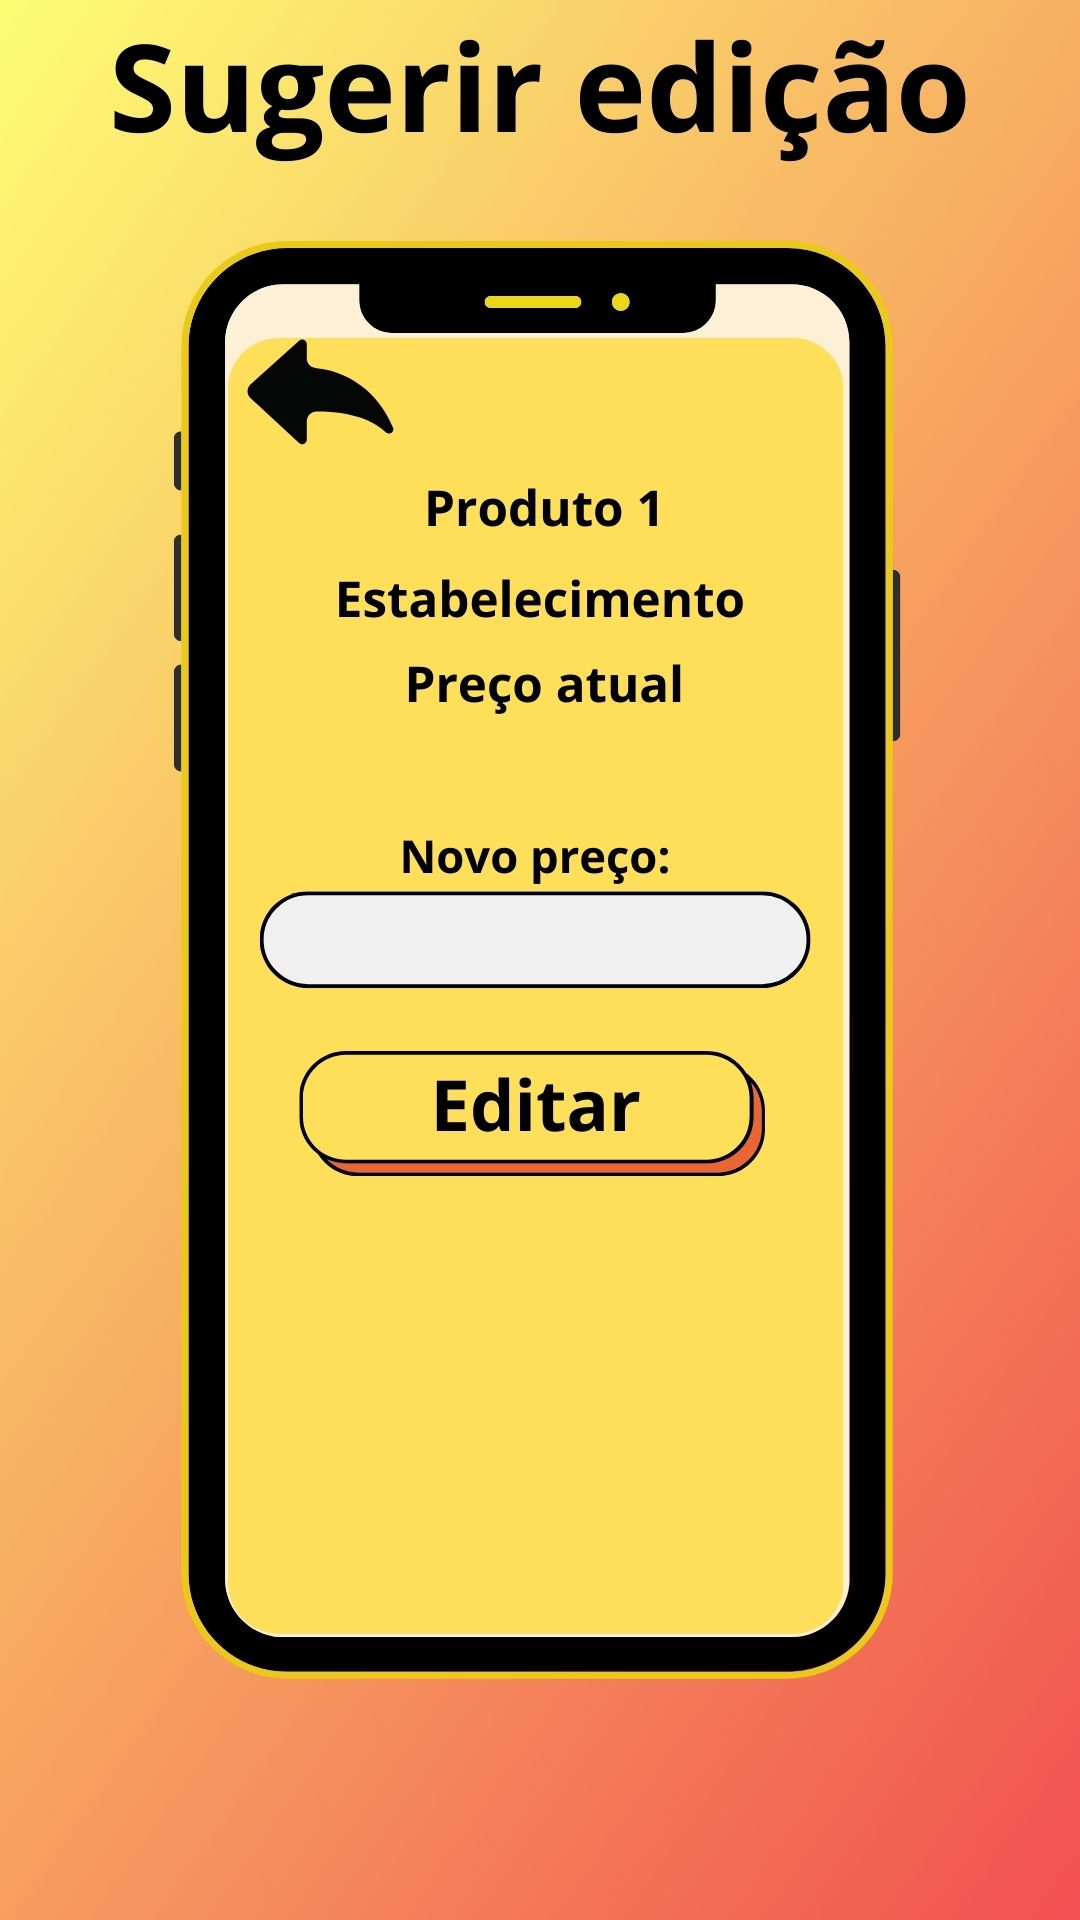
\includegraphics[width=\textwidth]{fig/telas/t_sugerir.jpg}
\footnotesize \centering
\par FONTE: O Autor (2024)
\end{figure}
\end{minipage}
 \\ \hline
\end{tabular}

\subsection*{\textbf{CRITÉRIOS DE ACEITAÇÃO}}

\begin{enumerate}[leftmargin=2cm]
    \item Deve mostrar as informações do produto.
    \item Deve permitir inserir um novo preço.
    \item Deve permitir sugerir um novo preço.
\end{enumerate}

\subsection*{\textbf{CRITÉRIOS DE ACEITAÇÃO - DETALHAMENTO}}
\textbf{Critério de contexto} (Válido como premissa para todos os critérios):

\begin{tabularx}{0.9\textwidth}{@{}l X }
\textbf{Dado que} & Sistema buscou ao menos 1 produto.\\ 
\textbf{E} & Usuário clicou em 1 produto.\\
\textbf{E} & Usuário clicou no botão de sugestão.
\end{tabularx}


\begin{tabularx}{0.9\textwidth}{|l|X|}
\multicolumn{2}{@{}l}{\textbf{1. Deve mostrar as informações do produto.}} \\ \hline
\textbf{Dado que} & Usuário está na tela de sugestão. \\ \hline
\textbf{Quanto} & Sistema carrega informações do produto. \\ \hline
\textbf{Então} & Sistema apresenta informações atuais do produto. \\ \hline
\end{tabularx}

\begin{tabularx}{0.9\textwidth}{|l|X|}
\multicolumn{2}{@{}l}{\textbf{2. Deve permitir inserir um novo preço.}} \\ \hline
\textbf{Dado que} & Usuário está na tela de sugestão. \\ \hline
\textbf{Quanto} & Usuário clica no campo "Novo preço". \\ \hline
\textbf{Então} & Sistema permite inserir novo preço. (R1) \\ \hline
\end{tabularx}

\begin{tabularx}{0.9\textwidth}{|l|X|}
\multicolumn{2}{@{}l}{\textbf{3. Deve permitir sugerir um novo preço.}} \\ \hline
\textbf{Dado que} & Usuário inseriu preço válido. (R1) \\ \hline
\textbf{Quanto} & Usuário clica no botão "Editar". \\ \hline
\textbf{Então} & Sistema cadastra nova sugestão. \\ \hline
\end{tabularx}

\subsection*{\textbf{REGRAS DE NEGÓCIO DA HISTÓRIA}}

\begin{itemize}
    \item[] R1 - Preço mínimo 0, preço máximo 999,999.
\end{itemize}


\section{Avaliar sugestão}%%%%%%%%%%%%%%%%%%%%%%%%%%%%%%%%%%%%%

\begin{tabular}{|ll|}
\hline
\multicolumn{2}{|c|}{\textbf{UC\nhist - \currentname}}    \\ \hline
\multicolumn{1}{|l|}{\textbf{Sendo}}     & um usuário \\ \hline
\multicolumn{1}{|l|}{\textbf{Quero}}     & avaliar uma sugestão de novo preço\\ \hline
\multicolumn{1}{|l|}{\textbf{Para}}      & para que o produto fique com o preço atualizado\\ \hline
\multicolumn{1}{|l|}{\textbf{Protótipo}} & 
\begin{minipage}{0.48\textwidth} 
\begin{figure}[H]
\caption{\label{fig:label} TELA AVALIAR SUGESTÃO}
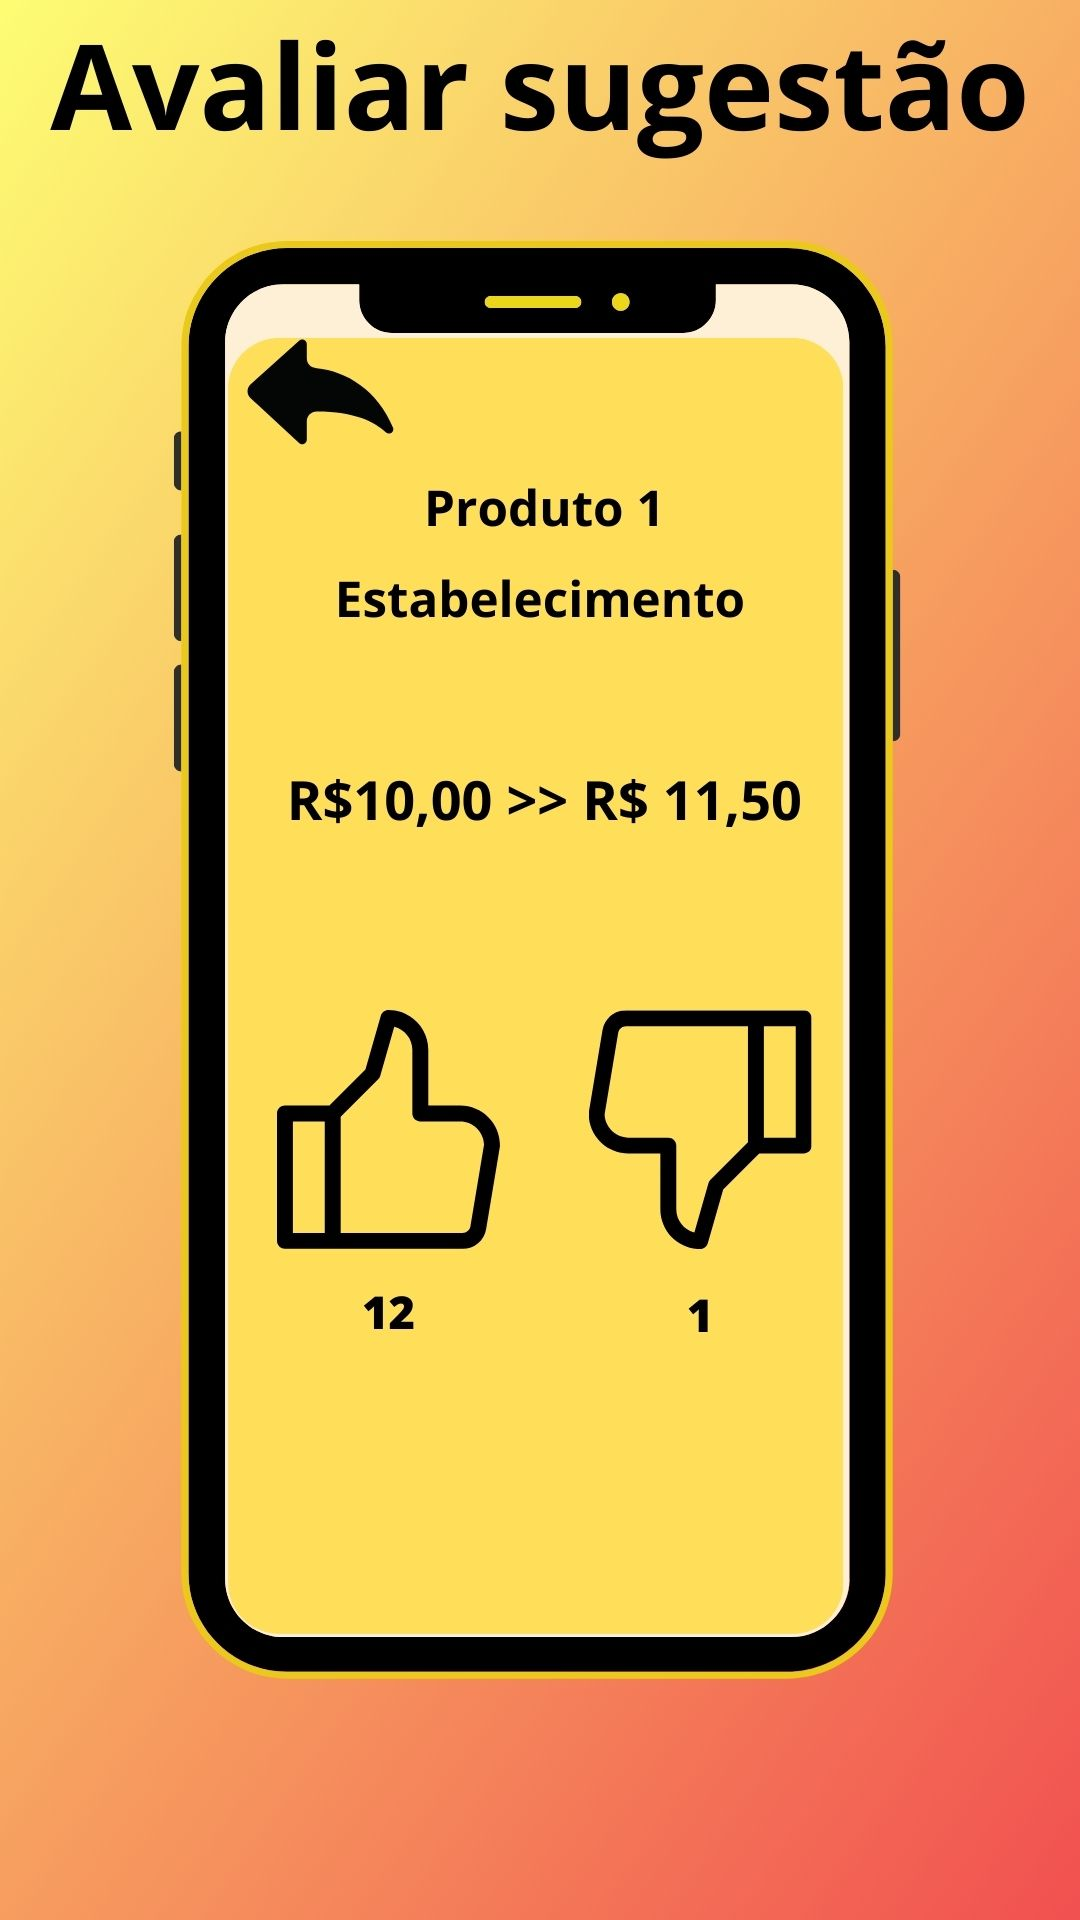
\includegraphics[width=\textwidth]{fig/telas/t_avaliar.jpg}
\footnotesize \centering
\par FONTE: O Autor (2024)
\end{figure}
\end{minipage}
 \\ \hline
\end{tabular}

\subsection*{\textbf{CRITÉRIOS DE ACEITAÇÃO}}

\begin{enumerate}[leftmargin=2cm]
    \item Deve mostrar as informações do produto atual e o novo preço sugerido.
    \item Deve permitir avaliar a sugestão com um positivo ou negativo.
    \item Deve atualizar o preço do produto se maioria das avaliações forem positivas.
\end{enumerate}

\subsection*{\textbf{CRITÉRIOS DE ACEITAÇÃO - DETALHAMENTO}}
\textbf{Critério de contexto} (Válido como premissa para todos os critérios):

\begin{tabularx}{0.9\textwidth}{@{}l X }
\textbf{Dado que} & Sistema buscou ao menos 1 produto. \\ 
\textbf{E} & Usuário clicou em 1 produto.
\end{tabularx}


\begin{tabularx}{0.9\textwidth}{|l|X|}
\multicolumn{2}{@{}l}{\textbf{\makecell[l]{1. Deve mostrar as informações do produto atual e o novo preço \\sugerido.}}} \\ \hline
\textbf{Dado que} & Usuário está na tela de avaliação. \\ \hline
\textbf{Quanto} & Sistema carrega informações do produto. \\ \hline
\textbf{Então} & Sistema apresenta informações da sugestão. \\ \hline
\end{tabularx}

\begin{tabularx}{0.9\textwidth}{|l|X|}
\multicolumn{2}{@{}l}{\textbf{2. Deve permitir avaliar a sugestão com um positivo ou negativo.}} \\ \hline
\textbf{Dado que} & Usuário está na tela de avaliação. \\ \hline
\textbf{Quanto} & Usuário avalia uma sugestão. \\ \hline
\textbf{Então} & Sistema atualiza números de avaliações. \\ \hline
\end{tabularx}

\begin{tabularx}{0.9\textwidth}{|l|X|}
\multicolumn{2}{@{}l}{\textbf{\makecell[l]{3. Deve atualizar o preço do produto se maioria das avaliações forem \\positivas.}}} \\ \hline
\textbf{Dado que} & Usuário está na tela de avaliação.  \\ \hline
\textbf{Quanto} & Usuário avalia uma sugestão. \\ \hline
\textbf{Então} & Sistema atualiza preço do produto. (R1) \\ \hline
\end{tabularx}

\subsection*{\textbf{REGRAS DE NEGÓCIO DA HISTÓRIA}}

\begin{itemize}
    \item[] R1 - Mais de 75\% das avaliações positivas.
\end{itemize}


\section{Cadastrar produto}%%%%%%%%%%%%%%%%%%%%%%%%%%%%%%%%%%%%%

\begin{tabular}{|ll|}
\hline
\multicolumn{2}{|c|}{\textbf{UC\nhist - \currentname}}    \\ \hline
\multicolumn{1}{|l|}{\textbf{Sendo}}     & um usuário \\ \hline
\multicolumn{1}{|l|}{\textbf{Quero}}     & cadastrar um novo produto\\ \hline
\multicolumn{1}{|l|}{\textbf{Para}}      & para que o produto apareça no sistema\\ \hline
\multicolumn{1}{|l|}{\textbf{Protótipo}} & 
\begin{minipage}{0.48\textwidth} 
\begin{figure}[H]
\caption{\label{fig:label} TELA CADASTRAR PRODUTO}
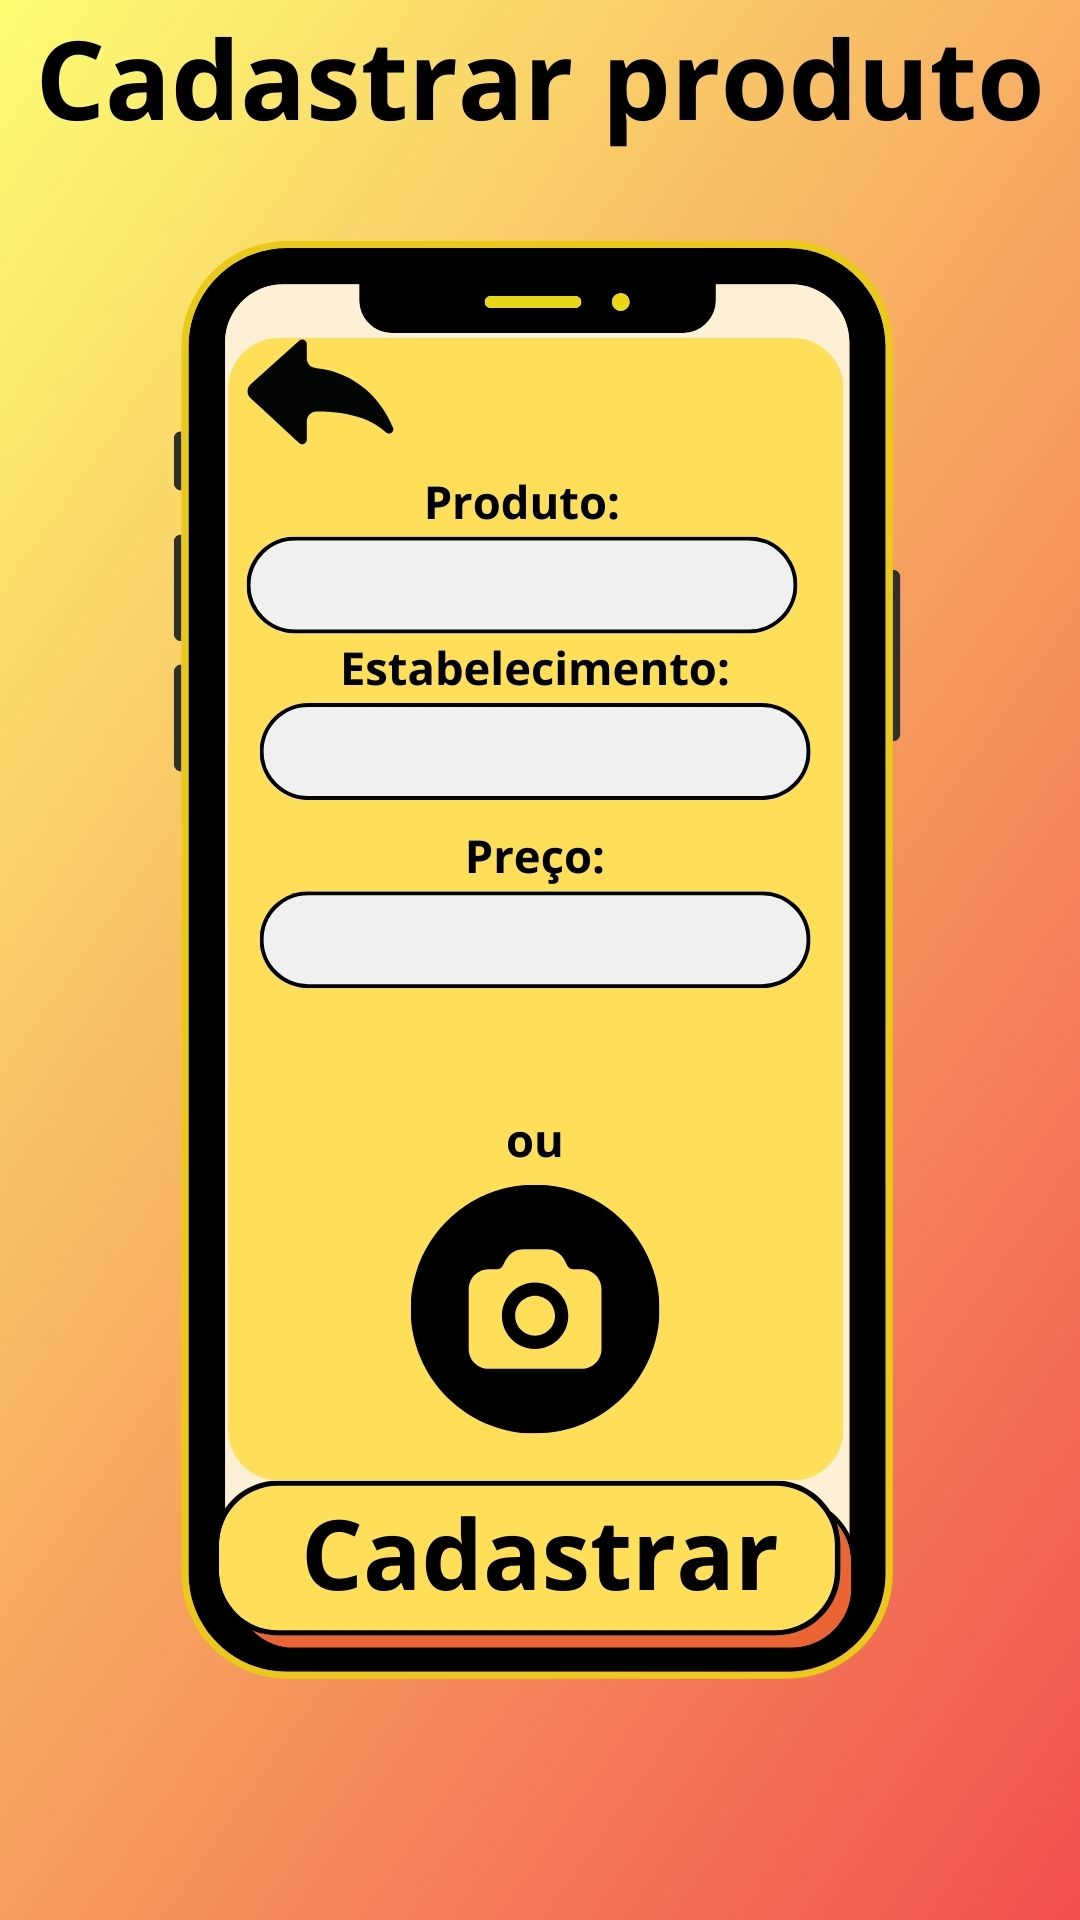
\includegraphics[width=\textwidth]{fig/telas/t_novproduto.jpg}
\footnotesize \centering
\par FONTE: O Autor (2024)
\end{figure}
\end{minipage}
 \\ \hline
\end{tabular}

\subsection*{\textbf{CRITÉRIOS DE ACEITAÇÃO}}

\begin{enumerate}[leftmargin=2cm]
    \item Deve permitir inserir o nome do produto, estabelecimento e preço do produto.
    \item Deve cadastrar o produto.
    \item Deve criar uma sugestão de novo preço pro produto caso já esteja cadastrado.
\end{enumerate}

\subsection*{\textbf{CRITÉRIOS DE ACEITAÇÃO - DETALHAMENTO}}
\textbf{Critério de contexto} (Válido como premissa para todos os critérios):

\begin{tabularx}{0.9\textwidth}{@{}l X }
 \textbf{Dado que} & Usuário esta logado \\ 
 \textbf{E} & Clicou no botão "Cadastrar produto".
\end{tabularx}

\begin{tabularx}{0.9\textwidth}{|l|X|}
\multicolumn{2}{@{}l}{\textbf{\makecell[l]{1. Deve permitir inserir o nome do produto, estabelecimento e \\preço do produto.}}} \\ \hline
\textbf{Dado que} & Usuário na tela de cadastro. \\ \hline
\textbf{Quanto} & Usuário clica em algum campo. \\ \hline
\textbf{Então} & Sistema permite edição. \\ \hline
\end{tabularx}

\begin{tabularx}{0.9\textwidth}{|l|X|}
\multicolumn{2}{@{}l}{\textbf{2. Deve cadastrar o produto.}} \\ \hline
\textbf{Dado que} & Usuário inseriu dados corretamente. (R1) (R2) \\ \hline
\textbf{Quanto} & Usuário clica no botão "Cadastrar". \\ \hline
\textbf{Então} & Sistema cadastra produto. \\ \hline
\end{tabularx}

\begin{tabularx}{0.9\textwidth}{|l|X|}
\multicolumn{2}{@{}l}{\textbf{\makecell[l]{3. Deve criar uma sugestão de novo preço pro produto caso já esteja \\cadastrado.}}} \\ \hline
\textbf{Dado que} & Usuário inseriu dados corretamente. (R1) (R2) \\ \hline
\textbf{Quanto} & Produto já cadastrado no estabelecimento. \\ \hline
\textbf{Então} & Sistema cadastra sugestão de preço. \\ \hline
\end{tabularx}

\subsection*{\textbf{REGRAS DE NEGÓCIO DA HISTÓRIA}}

\begin{itemize}
    \item[] R1 - Localização correta no mapa.
    \item[] R2 - Preço mínimo 0, preço máximo 999,999.
\end{itemize}


\section{Digitalizar nota}%%%%%%%%%%%%%%%%%%%%%%%%%%%%%%%%%%%%%

\begin{tabular}{|ll|}
\hline
\multicolumn{2}{|c|}{\textbf{UC\nhist - \currentname}}    \\ \hline
\multicolumn{1}{|l|}{\textbf{Sendo}}     & um usuário \\ \hline
\multicolumn{1}{|l|}{\textbf{Quero}}     & digitalizar uma nota\\ \hline
\multicolumn{1}{|l|}{\textbf{Para}}      & para inserir automaticamente os produtos no sistema\\ \hline
\multicolumn{1}{|l|}{\textbf{Protótipo}} & 
\begin{minipage}{0.48\textwidth} 
\begin{figure}[H]
\caption{\label{fig:label} TELA DIGITALIZAR}
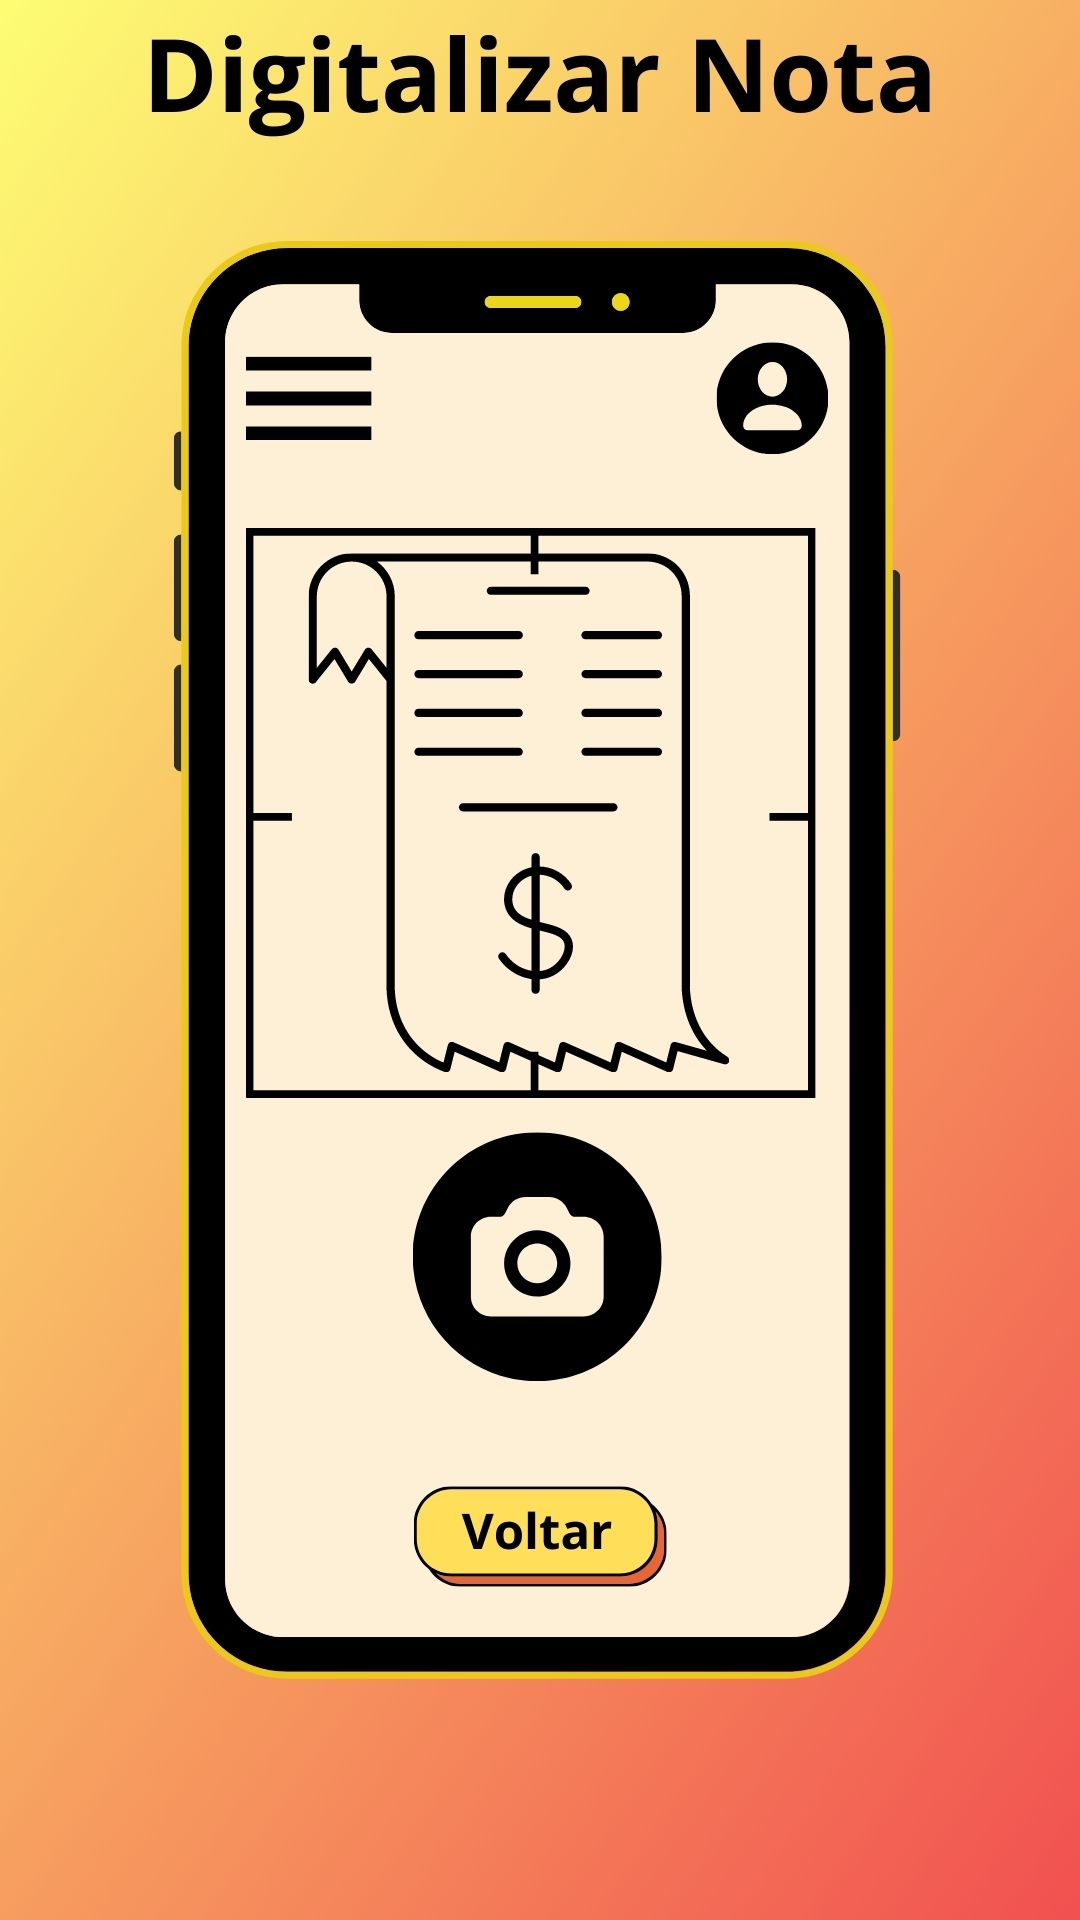
\includegraphics[width=\textwidth]{fig/telas/t_digitaliza.jpg}
\footnotesize \centering
\par FONTE: O Autor (2024)
\end{figure}
\end{minipage}
 \\ \hline
\end{tabular}

\subsection*{\textbf{CRITÉRIOS DE ACEITAÇÃO}}

\begin{enumerate}[leftmargin=2cm]
    \item Deve permitir tirar uma foto de uma nota fiscal.
    \item Deve digitalizar os itens da nota em texto.
\end{enumerate}

\subsection*{\textbf{CRITÉRIOS DE ACEITAÇÃO - DETALHAMENTO}}
\textbf{Critério de contexto} (Válido como premissa para todos os critérios):

\begin{tabularx}{0.9\textwidth}{@{}l X }
\textbf{Dado que} & Usuário esta logado \\ 
\textbf{E} & Clicou no botão "Cadastrar produto".\\
\textbf{E} & Clicou no ícone de nota fiscal.
\end{tabularx}


\begin{tabularx}{0.9\textwidth}{|l|X|}
\multicolumn{2}{@{}l}{\textbf{1. Deve permitir tirar uma foto de uma nota fiscal.}} \\ \hline
\textbf{Dado que} & Usuário está na tela de nota fiscal. \\ \hline
\textbf{Quanto} & Usuário clica no ícone de camera. \\ \hline
\textbf{Então} & Sistema permite escanear uma foto. \\ \hline
\end{tabularx}

\begin{tabularx}{0.9\textwidth}{|l|X|}
\multicolumn{2}{@{}l}{\textbf{2. Deve digitalizar os itens da nota em texto.}} \\ \hline
\textbf{Dado que} & Usuário escaneou nota corretamente. (R1) \\ \hline
\textbf{Quanto} & Usuário clica no ícone de camera. \\ \hline
\textbf{Então} & Sistema redireciona para tela de confirmação. \\ \hline
\end{tabularx}

\subsection*{\textbf{REGRAS DE NEGÓCIO DA HISTÓRIA}}

\begin{itemize}
    \item[] R1 - QR Code da nota fiscal encontrada.
\end{itemize}

\section{Confirmar digitalização}%%%%%%%%%%%%%%%%%%%%%%%%%%%%%%%%%%%%%

\begin{tabular}{|ll|}
\hline
\multicolumn{2}{|c|}{\textbf{UC\nhist - \currentname}}    \\ \hline
\multicolumn{1}{|l|}{\textbf{Sendo}}     & um usuário \\ \hline
\multicolumn{1}{|l|}{\textbf{Quero}}     & confirmar a digitalização\\ \hline
\multicolumn{1}{|l|}{\textbf{Para}}      & para corrigir eventuais erros inseridos pelo sistema\\ \hline
\multicolumn{1}{|l|}{\textbf{Protótipo}} & 
\begin{minipage}{0.48\textwidth} 
\begin{figure}[H]
\caption{\label{fig:label} TELA DIGITALIZAÇÃO}
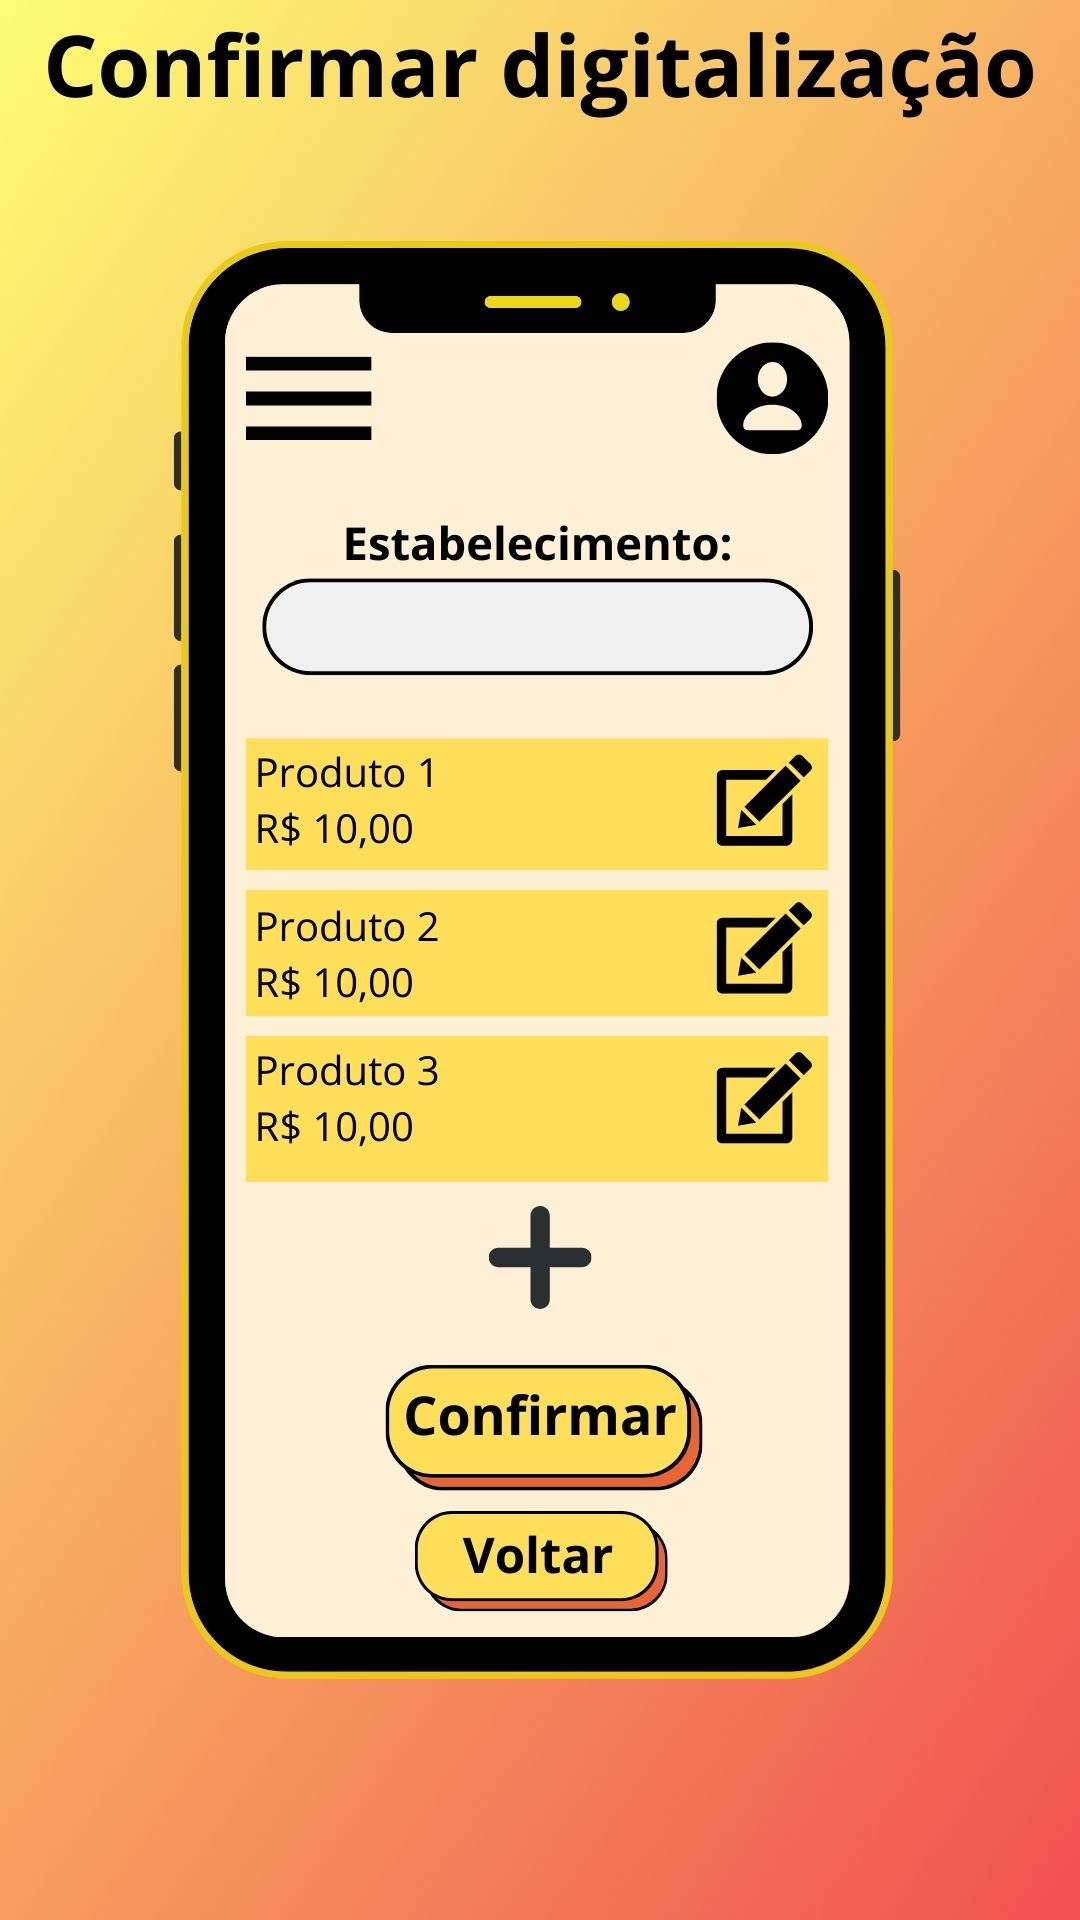
\includegraphics[width=\textwidth]{fig/telas/t_confdigitaliza.jpg}
\footnotesize \centering
\par FONTE: O Autor (2024)
\end{figure}
\end{minipage}
 \\ \hline
\end{tabular}

\subsection*{\textbf{CRITÉRIOS DE ACEITAÇÃO}}

\begin{enumerate}[leftmargin=2cm]
    \item Deve permitir inserir o estabelecimento da nota.
    \item Deve permitir alterar os produtos digitalizados pelo sistema.
    \item Deve permitir adicionar mais produtos.
    \item Deve cadastrar os produtos.
    \item Deve criar uma sugestão de novo preço pro produto caso já esteja cadastrado.
\end{enumerate}

\subsection*{\textbf{CRITÉRIOS DE ACEITAÇÃO - DETALHAMENTO}}
\textbf{Critério de contexto} (Válido como premissa para todos os critérios):

\begin{tabularx}{0.9\textwidth}{@{}l X }
\textbf{Dado que} & Usuário esta logado \\ 
\textbf{E} & Clicou no botão "Cadastrar produto".\\
\textbf{E} & Clicou no ícone de nota fiscal.\\
\textbf{E} & Escaneou uma nota válida.
\end{tabularx}


\begin{tabularx}{0.9\textwidth}{|l|X|}
\multicolumn{2}{@{}l}{\textbf{1. Deve permitir inserir o estabelecimento da nota.}} \\ \hline
\textbf{Dado que} & Usuário está na tela de confirmação. \\ \hline
\textbf{Quanto} & Usuário clica no campo "Estabelecimento". \\ \hline
\textbf{Então} & Sistema permite selecionar no mapa a localiação. \\ \hline
\end{tabularx}

\begin{tabularx}{0.9\textwidth}{|l|X|}
\multicolumn{2}{@{}l}{\textbf{2. Deve permitir alterar os produtos digitalizados pelo sistema.}} \\ \hline
\textbf{Dado que} & Usuário está na tela de confirmação. \\ \hline
\textbf{Quanto} & Usuário clica no ícone de edição. \\ \hline
\textbf{Então} & Sistema apresenta formulário de edição. \\ \hline
\end{tabularx}

\begin{tabularx}{0.9\textwidth}{|l|X|}
\multicolumn{2}{@{}l}{\textbf{3. Deve permitir adicionar mais produtos.}} \\ \hline
\textbf{Dado que} & Usuário está na tela de confirmação. \\ \hline
\textbf{Quanto} & Usuário clica no ícone de adição. \\ \hline
\textbf{Então} & Sistema apresenta formulário de adição. \\ \hline
\end{tabularx}

\begin{tabularx}{0.9\textwidth}{|l|X|}
\multicolumn{2}{@{}l}{\textbf{4. Deve cadastrar os produtos.}} \\ \hline
\textbf{Dado que} & Usuário está na tela de confirmação. \\ \hline
\textbf{Quanto} & Usuário clica no ícone "Confirmar". \\ \hline
\textbf{Então} & Sistema cadastra produtos. \\ \hline
\end{tabularx}

\begin{tabularx}{0.9\textwidth}{|l|X|}
\multicolumn{2}{@{}l}{\textbf{\makecell[l]{5. Deve criar uma sugestão de novo preço pro produto caso já esteja \\cadastrado.}}} \\ \hline
\textbf{Dado que} & Usuário clica no ícone "Confirmar".\\ \hline
\textbf{Quanto} & Produto já cadastrado. \\ \hline
\textbf{Então} & Sistema cadastra sugestão de novo preço. \\ \hline
\end{tabularx}


\section{Menu perfil}%%%%%%%%%%%%%%%%%%%%%%%%%%%%%%%%%%%%%

\begin{tabular}{|ll|}
\hline
\multicolumn{2}{|c|}{\textbf{UC\nhist - \currentname}}    \\ \hline
\multicolumn{1}{|l|}{\textbf{Sendo}}     & um usuário \\ \hline
\multicolumn{1}{|l|}{\textbf{Quero}}     & visualizar os detalhes do meu perfil\\ \hline
\multicolumn{1}{|l|}{\textbf{Para}}      & alterar minha senha ou foto\\ \hline
\multicolumn{1}{|l|}{\textbf{Protótipo}} & 
\begin{minipage}{0.48\textwidth} 
\begin{figure}[H]
\caption{\label{fig:label} TELA PERFIL}
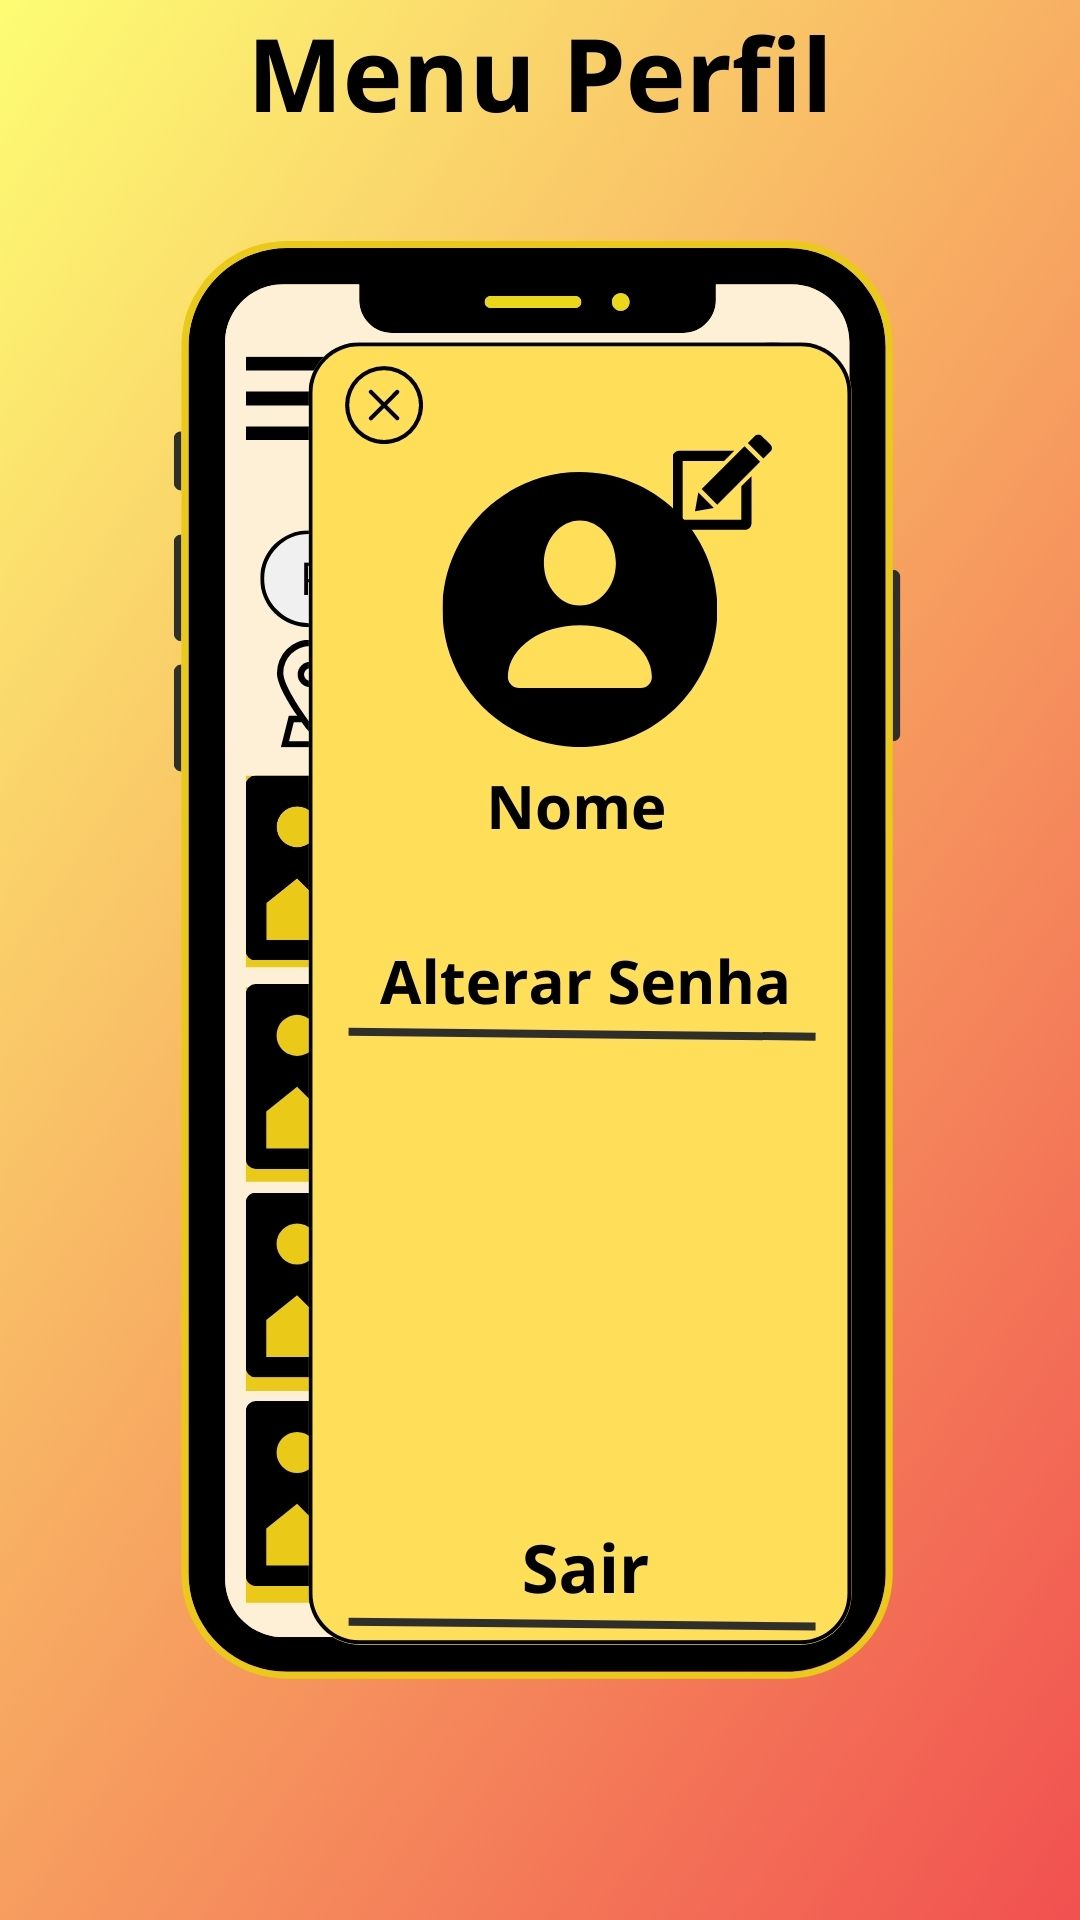
\includegraphics[width=\textwidth]{fig/telas/t_mperfil.jpg}
\footnotesize \centering
\par FONTE: O Autor (2024)
\end{figure}
\end{minipage}
 \\ \hline
\end{tabular}

\subsection*{\textbf{CRITÉRIOS DE ACEITAÇÃO}}

\begin{enumerate}[leftmargin=2cm]
    \item Deve mostrar as informações do usuário logado.
    \item Deve permitir alterar a foto.
    \item Deve permitir alterar a senha.
\end{enumerate}

\subsection*{\textbf{CRITÉRIOS DE ACEITAÇÃO - DETALHAMENTO}}
\textbf{Critério de contexto} (Válido como premissa para todos os critérios):

\begin{tabularx}{0.9\textwidth}{@{}l X }
 \textbf{Dado que} & Usuário logado. \\ 
 \textbf{E} & Clicou no menu lateral.
\end{tabularx}


\begin{tabularx}{0.9\textwidth}{|l|X|}
\multicolumn{2}{@{}l}{\textbf{1. Deve mostrar as informações do usuário logado.}} \\ \hline
\textbf{Dado que} & Usuário está na tela de perfil. \\ \hline
\textbf{Quanto} & Sistema carrega informações do usuário. \\ \hline
\textbf{Então} & Sistema apresenta informações do usuário. \\ \hline
\end{tabularx}

\begin{tabularx}{0.9\textwidth}{|l|X|}
\multicolumn{2}{@{}l}{\textbf{2. Deve permitir alterar a foto.}} \\ \hline
\textbf{Dado que} & Usuário está na tela de perfil. \\ \hline
\textbf{Quanto} & Usuário clica no ícone de camera. \\ \hline
\textbf{Então} & Sistema permite atualizar foto. (R1) \\ \hline
\end{tabularx}

\begin{tabularx}{0.9\textwidth}{|l|X|}
\multicolumn{2}{@{}l}{\textbf{3. Deve permitir alterar a senha.}} \\ \hline
\textbf{Dado que} & Usuário está na tela de perfil. \\ \hline
\textbf{Quanto} & Usuário clica em "Alterar senha". \\ \hline
\textbf{Então} & Sistema redireciona para tela de alteração. \\ \hline
\end{tabularx}

\subsection*{\textbf{REGRAS DE NEGÓCIO DA HISTÓRIA}}

\begin{itemize}
    \item[] R1 - Tamanho máximo do arquivo 5mb.
\end{itemize}



\section{Alterar senha}%%%%%%%%%%%%%%%%%%%%%%%%%%%%%%%%%%%%%

\begin{tabular}{|ll|}
\hline
\multicolumn{2}{|c|}{\textbf{UC\nhist - \currentname}}    \\ \hline
\multicolumn{1}{|l|}{\textbf{Sendo}}     & um usuário \\ \hline
\multicolumn{1}{|l|}{\textbf{Quero}}     & alterar minha senha\\ \hline
\multicolumn{1}{|l|}{\textbf{Para}}      & alterar minha senha atual para uma nova\\ \hline
\multicolumn{1}{|l|}{\textbf{Protótipo}} & 
\begin{minipage}{0.48\textwidth} 
\begin{figure}[H]
\caption{\label{fig:label} TELA ALTERAR SENHA}
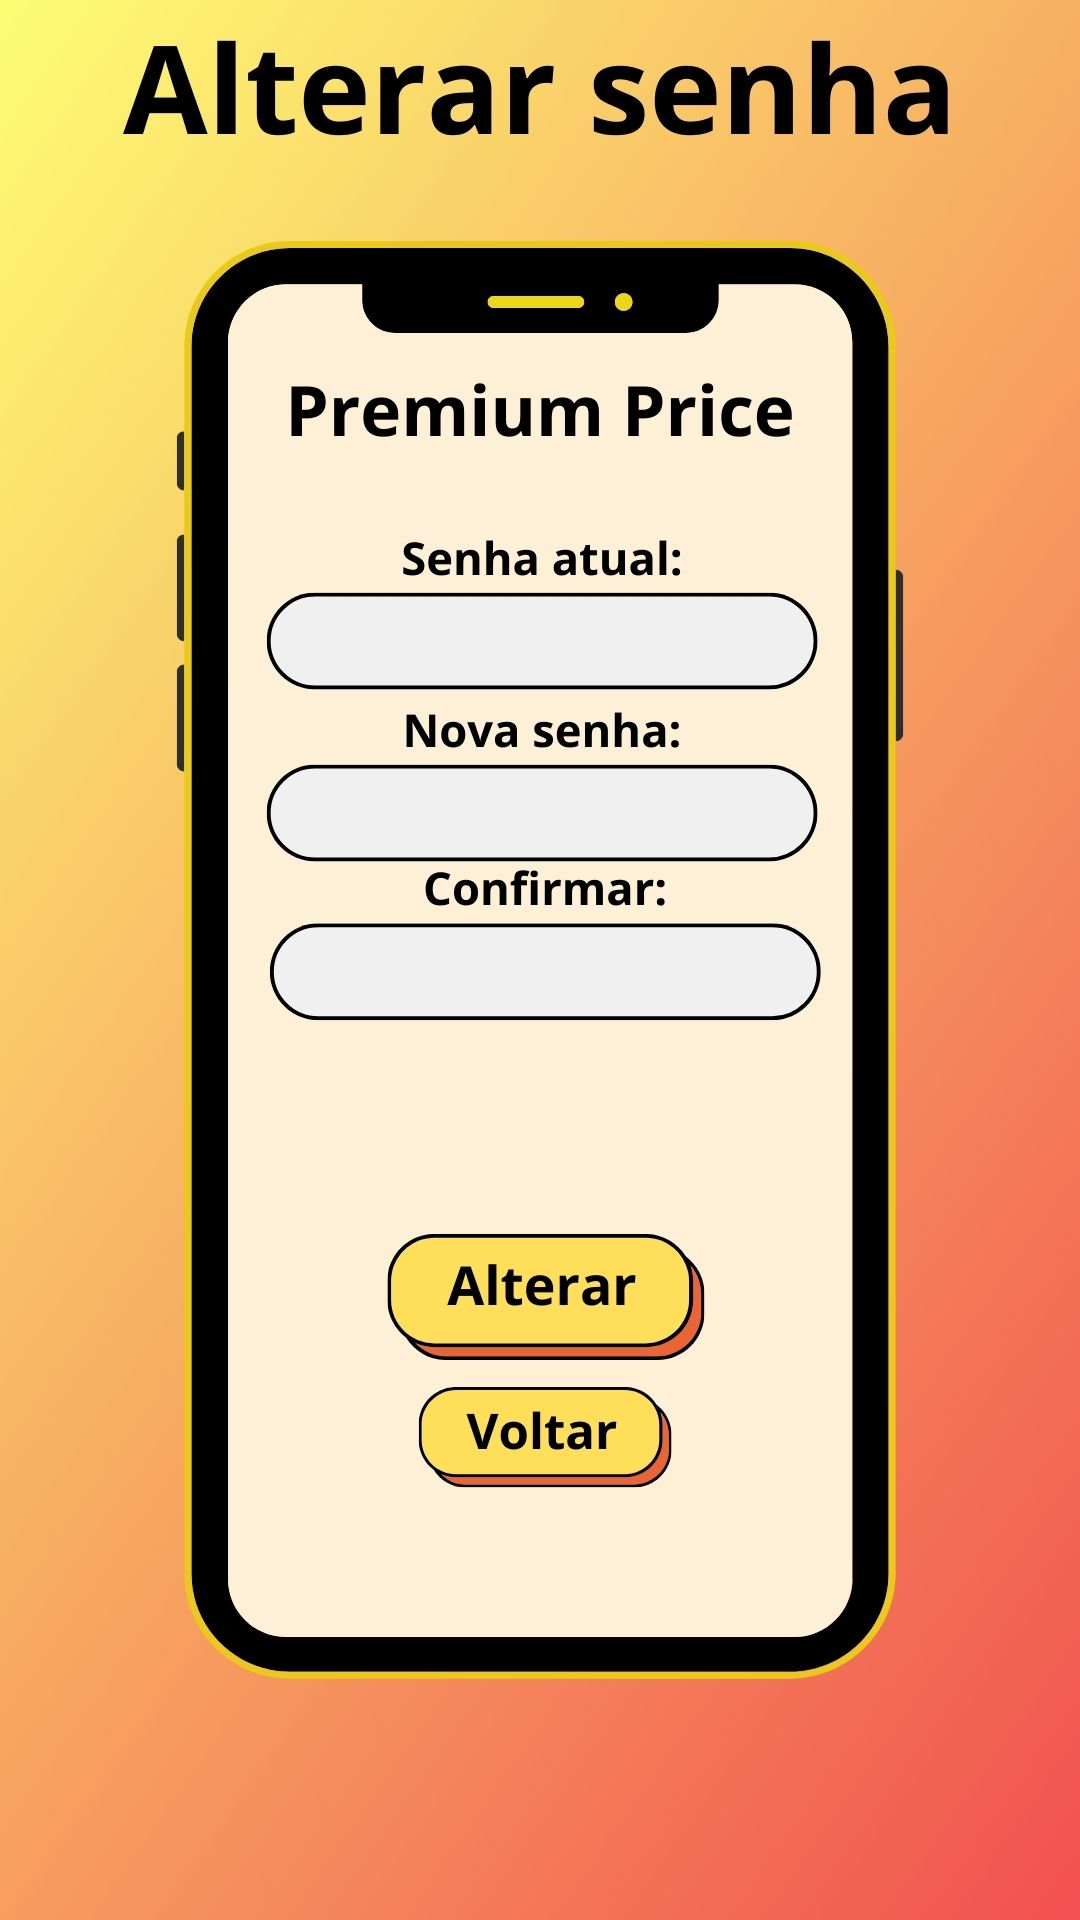
\includegraphics[width=\textwidth]{fig/telas/t_altsenha.jpg}
\footnotesize \centering
\par FONTE: O Autor (2024)
\end{figure}
\end{minipage}
 \\ \hline
\end{tabular}

\subsection*{\textbf{CRITÉRIOS DE ACEITAÇÃO}}

\begin{enumerate}[leftmargin=2cm]
    \item Deve permitir inserir a senha atual e uma nova senha.
    \item Deve permitir alterar a senha caso a senha atual seja inserida corretamente.
\end{enumerate}

\subsection*{\textbf{CRITÉRIOS DE ACEITAÇÃO - DETALHAMENTO}}
\textbf{Critério de contexto} (Válido como premissa para todos os critérios):

\begin{tabularx}{0.9\textwidth}{@{}l X }
\textbf{Dado que} & Usuário logado. \\ 
\textbf{E} & Clicou no menu lateral.\\
\textbf{E} & Clicou em alterar senha.
\end{tabularx}


\begin{tabularx}{0.9\textwidth}{|l|X|}
\multicolumn{2}{@{}l}{\textbf{1. Deve permitir inserir a senha atual e uma nova senha.}} \\ \hline
\textbf{Dado que} & Usuário está na tela de alterar senha. \\ \hline
\textbf{Quanto} & Usuário clica nos campos de senha. \\ \hline
\textbf{Então} & Sistema permite inserir dado. \\ \hline
\end{tabularx}

\begin{tabularx}{0.9\textwidth}{|l|X|}
\multicolumn{2}{@{}l}{\textbf{\makecell[l]{2. Deve permitir alterar a senha caso a senha atual seja inserida \\corretamente.}}} \\ \hline
\textbf{Dado que} & Usuário inseriu campos corretamente. (R1) (R2) (R3) \\ \hline
\textbf{Quanto} & Usuário clicou em "Alterar". \\ \hline
\textbf{Então} & Sistema atualiza senha do usuário. \\ \hline
\end{tabularx}

\subsection*{\textbf{REGRAS DE NEGÓCIO DA HISTÓRIA}}

\begin{itemize}
    \item[] R1 - Senha atual válida.
    \item[] R2 - Novas e confirmação iguais.
    \item[] R3 - Tamanho máximo do texto 256 caracteres.
\end{itemize}




\section{Logar no sistema}%%%%%%%%%%%%%%%%%%%%%%%%%%%%%%%%%%%%%

\begin{tabular}{|ll|}
\hline
\multicolumn{2}{|c|}{\textbf{UC\nhist - \currentname}}    \\ \hline
\multicolumn{1}{|l|}{\textbf{Sendo}}     & um usuário \\ \hline
\multicolumn{1}{|l|}{\textbf{Quero}}     & logar no sistema\\ \hline
\multicolumn{1}{|l|}{\textbf{Para}}      & poder avaliar e sugerir novos preços para os produtos\\ \hline
\multicolumn{1}{|l|}{\textbf{Protótipo}} & 
\begin{minipage}{0.48\textwidth} 
\begin{figure}[H]
\caption{\label{fig:label} TELA LOGIN}
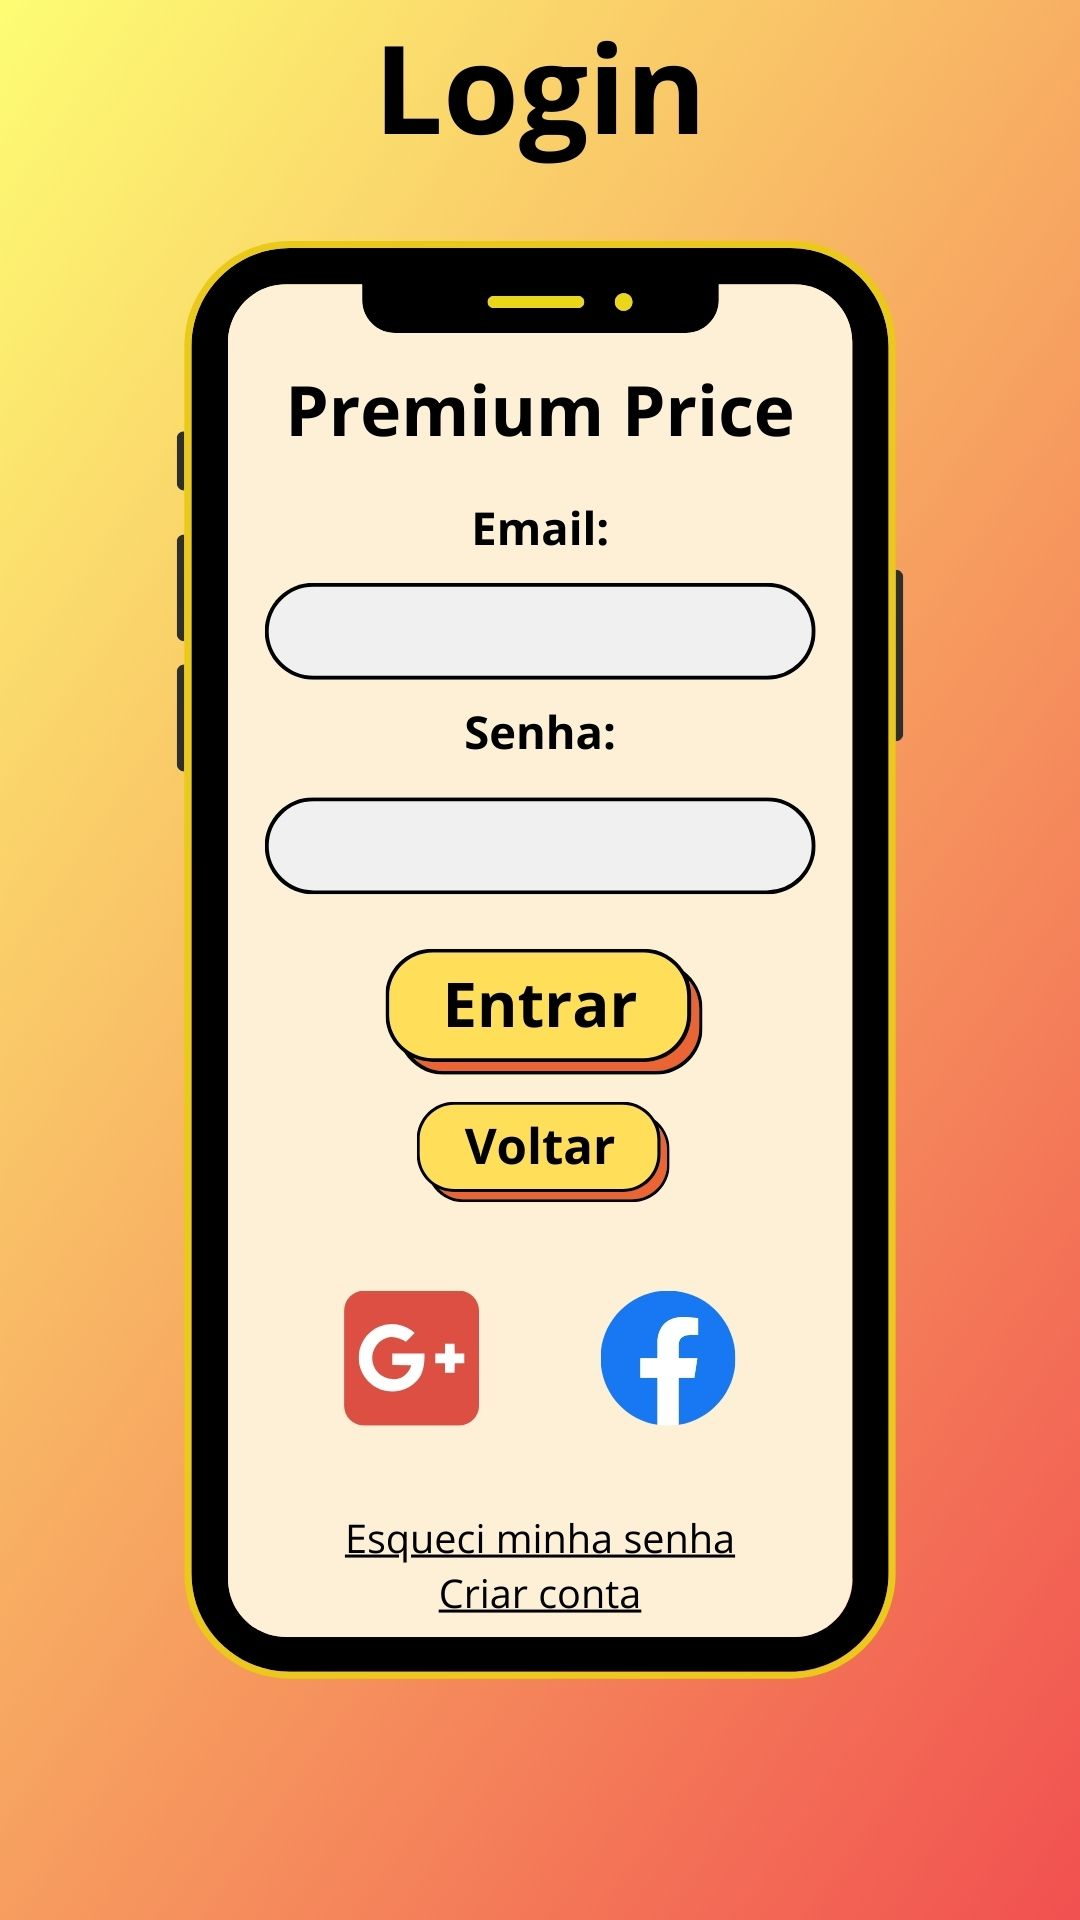
\includegraphics[width=\textwidth]{fig/telas/t_login.jpg}
\footnotesize \centering
\par FONTE: O Autor (2024)
\end{figure}
\end{minipage}
 \\ \hline
\end{tabular}

\subsection*{\textbf{CRITÉRIOS DE ACEITAÇÃO}}

\begin{enumerate}[leftmargin=2cm]
    \item Deve permitir inserir email e senha.
    \item Deve permitir fazer cadastro pela conta Google ou Facebook.
    \item Deve permitir recuperar senha.
    \item Deve permitir acessar formulário de cadastro.
    \item Deve permitir logar no sistema.
\end{enumerate}

\subsection*{\textbf{CRITÉRIOS DE ACEITAÇÃO - DETALHAMENTO}}
\textbf{Critério de contexto} (Válido como premissa para todos os critérios):

\begin{tabularx}{0.9\textwidth}{@{}l X }
 \textbf{Dado que} & Usuário clicou no botão "Login". \\ 
\end{tabularx}


\begin{tabularx}{0.9\textwidth}{|l|X|}
\multicolumn{2}{@{}l}{\textbf{1. Deve permitir inserir email e senha.}} \\ \hline
\textbf{Dado que} & Usuário está na tela de login. \\ \hline
\textbf{Quanto} & Usuário clica nos campos. \\ \hline
\textbf{Então} & Sistema permite inserir dado. (R1) (R2) \\ \hline
\end{tabularx}

\begin{tabularx}{0.9\textwidth}{|l|X|}
\multicolumn{2}{@{}l}{\textbf{2. Deve permitir fazer cadastro pela conta Google ou Facebook.}} \\ \hline
\textbf{Dado que} & Usuário está na tela de login. \\ \hline
\textbf{Quanto} & Usuário clica no botão Google ou Facebook \\ \hline
\textbf{Então} & Sistema redireciona para login externo. \\ \hline
\end{tabularx}

\begin{tabularx}{0.9\textwidth}{|l|X|}
\multicolumn{2}{@{}l}{\textbf{3. Deve permitir recuperar senha.}} \\ \hline
\textbf{Dado que} & Usuário está na tela de login. \\ \hline
\textbf{Quanto} & Usuário clica em "Esqueci minha senha". \\ \hline
\textbf{Então} & Sistema redireciona para tela de recuperação. \\ \hline
\end{tabularx}

\begin{tabularx}{0.9\textwidth}{|l|X|}
\multicolumn{2}{@{}l}{\textbf{4. Deve permitir acessar formulário de cadastro.}} \\ \hline
\textbf{Dado que} & Usuário está na tela de login. \\ \hline
\textbf{Quanto} & Usuário clica em "Criar conta". \\ \hline
\textbf{Então} & Sistema redireciona para tela de cadastro. \\ \hline
\end{tabularx}

\begin{tabularx}{0.9\textwidth}{|l|X|}
\multicolumn{2}{@{}l}{\textbf{5. Deve permitir logar no sistema.}} \\ \hline
\textbf{Dado que} & Usuário inseriu credenciais corretas. (R3) \\ \hline
\textbf{Quanto} & Usuário clica em "Entrar". \\ \hline
\textbf{Então} & Sistema autentica usuário e redireciona para tela inicial. \\ \hline
\end{tabularx}

\subsection*{\textbf{REGRAS DE NEGÓCIO DA HISTÓRIA}}

\begin{itemize}
    \item[] R1 - Tamanho maximo do texto 256 caracteres.
    \item[] R2 - Email válido.
    \item[] R3 - Usuário cadastrado no banco de dados.
\end{itemize}

\section{Criar conta}%%%%%%%%%%%%%%%%%%%%%%%%%%%%%%%%%%%%%

\begin{tabular}{|ll|}
\hline
\multicolumn{2}{|c|}{\textbf{UC\nhist - \currentname}}    \\ \hline
\multicolumn{1}{|l|}{\textbf{Sendo}}     & um usuário \\ \hline
\multicolumn{1}{|l|}{\textbf{Quero}}     & cadastrar no sistema\\ \hline
\multicolumn{1}{|l|}{\textbf{Para}}      & criar uma conta para logar no sistema\\ \hline
\multicolumn{1}{|l|}{\textbf{Protótipo}} & 
\begin{minipage}{0.48\textwidth} 
\begin{figure}[H]
\caption{\label{fig:label} TELA CADASTRO}
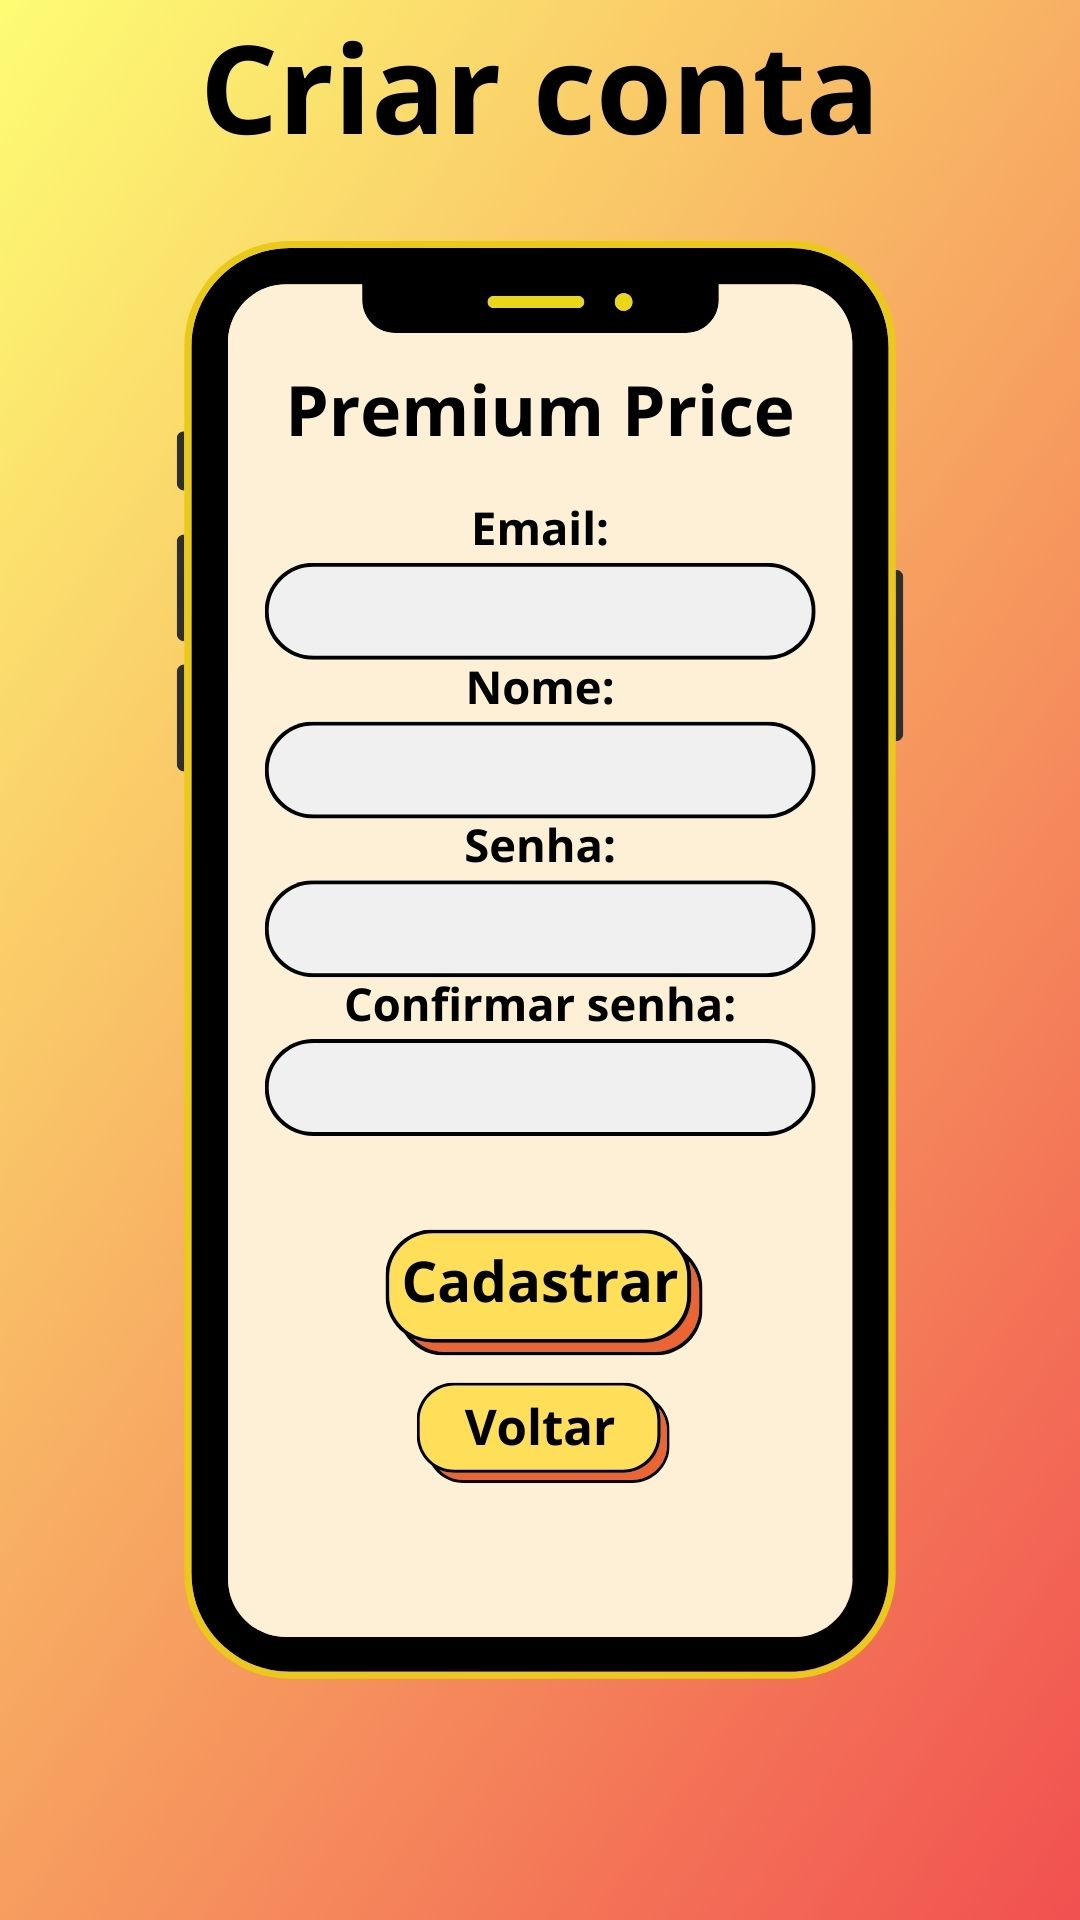
\includegraphics[width=\textwidth]{fig/telas/t_cadastro.jpg}
\footnotesize \centering
\par FONTE: O Autor (2024)
\end{figure}
\end{minipage}
 \\ \hline
\end{tabular}

\subsection*{\textbf{CRITÉRIOS DE ACEITAÇÃO}}

\begin{enumerate}[leftmargin=2cm]
    \item Deve permitir inserir email, nome e senha.
    \item Deve fazer cadastro no sistema.
\end{enumerate}

\subsection*{\textbf{CRITÉRIOS DE ACEITAÇÃO - DETALHAMENTO}}
\textbf{Critério de contexto} (Válido como premissa para todos os critérios):

\begin{tabularx}{0.9\textwidth}{@{}l X }
\textbf{Dado que} & Usuário clicou no botão "Criar conta". \\ 
\end{tabularx}


\begin{tabularx}{0.9\textwidth}{|l|X|}
\multicolumn{2}{@{}l}{\textbf{1. Deve permitir inserir email, nome e senha.}} \\ \hline
\textbf{Dado que} & Usuário está na tela de cadastro. \\ \hline
\textbf{Quanto} & Usuário clica nos campos. \\ \hline
\textbf{Então} & Sistema permite inserir dado. \\ \hline
\end{tabularx}

\begin{tabularx}{0.9\textwidth}{|l|X|}
\multicolumn{2}{@{}l}{\textbf{2. Deve fazer cadastro no sistema.}} \\ \hline
\textbf{Dado que} & Usuário preencheu corretamente. (R1) (R2) (R3) (R4) \\ \hline
\textbf{Quanto} & Usuário clica em "Cadastrar". \\ \hline
\textbf{Então} & Sistema cadastra novo usuário. \\ \hline
\end{tabularx}

\subsection*{\textbf{REGRAS DE NEGÓCIO DA HISTÓRIA}}

\begin{itemize}
    \item[] R1 - Email válido.
    \item[] R2 - Tamanho máximo do texto 256 caracteres.
    \item[] R3 - Senha e confirmação iguais.
    \item[] R4 - Usuário ainda não cadastrado.
\end{itemize}


\section{Recuperar senha}%%%%%%%%%%%%%%%%%%%%%%%%%%%%%%%%%%%%%

\begin{tabular}{|ll|}
\hline
\multicolumn{2}{|c|}{\textbf{UC\nhist - \currentname}}    \\ \hline
\multicolumn{1}{|l|}{\textbf{Sendo}}     & um usuário \\ \hline
\multicolumn{1}{|l|}{\textbf{Quero}}     & recuperar minha senha\\ \hline
\multicolumn{1}{|l|}{\textbf{Para}}      & acessar o sistema\\ \hline
\multicolumn{1}{|l|}{\textbf{Protótipo}} & 
\begin{minipage}{0.48\textwidth} 
\begin{figure}[H]
\caption{\label{fig:label} TELA RECUPERAR SENHA}
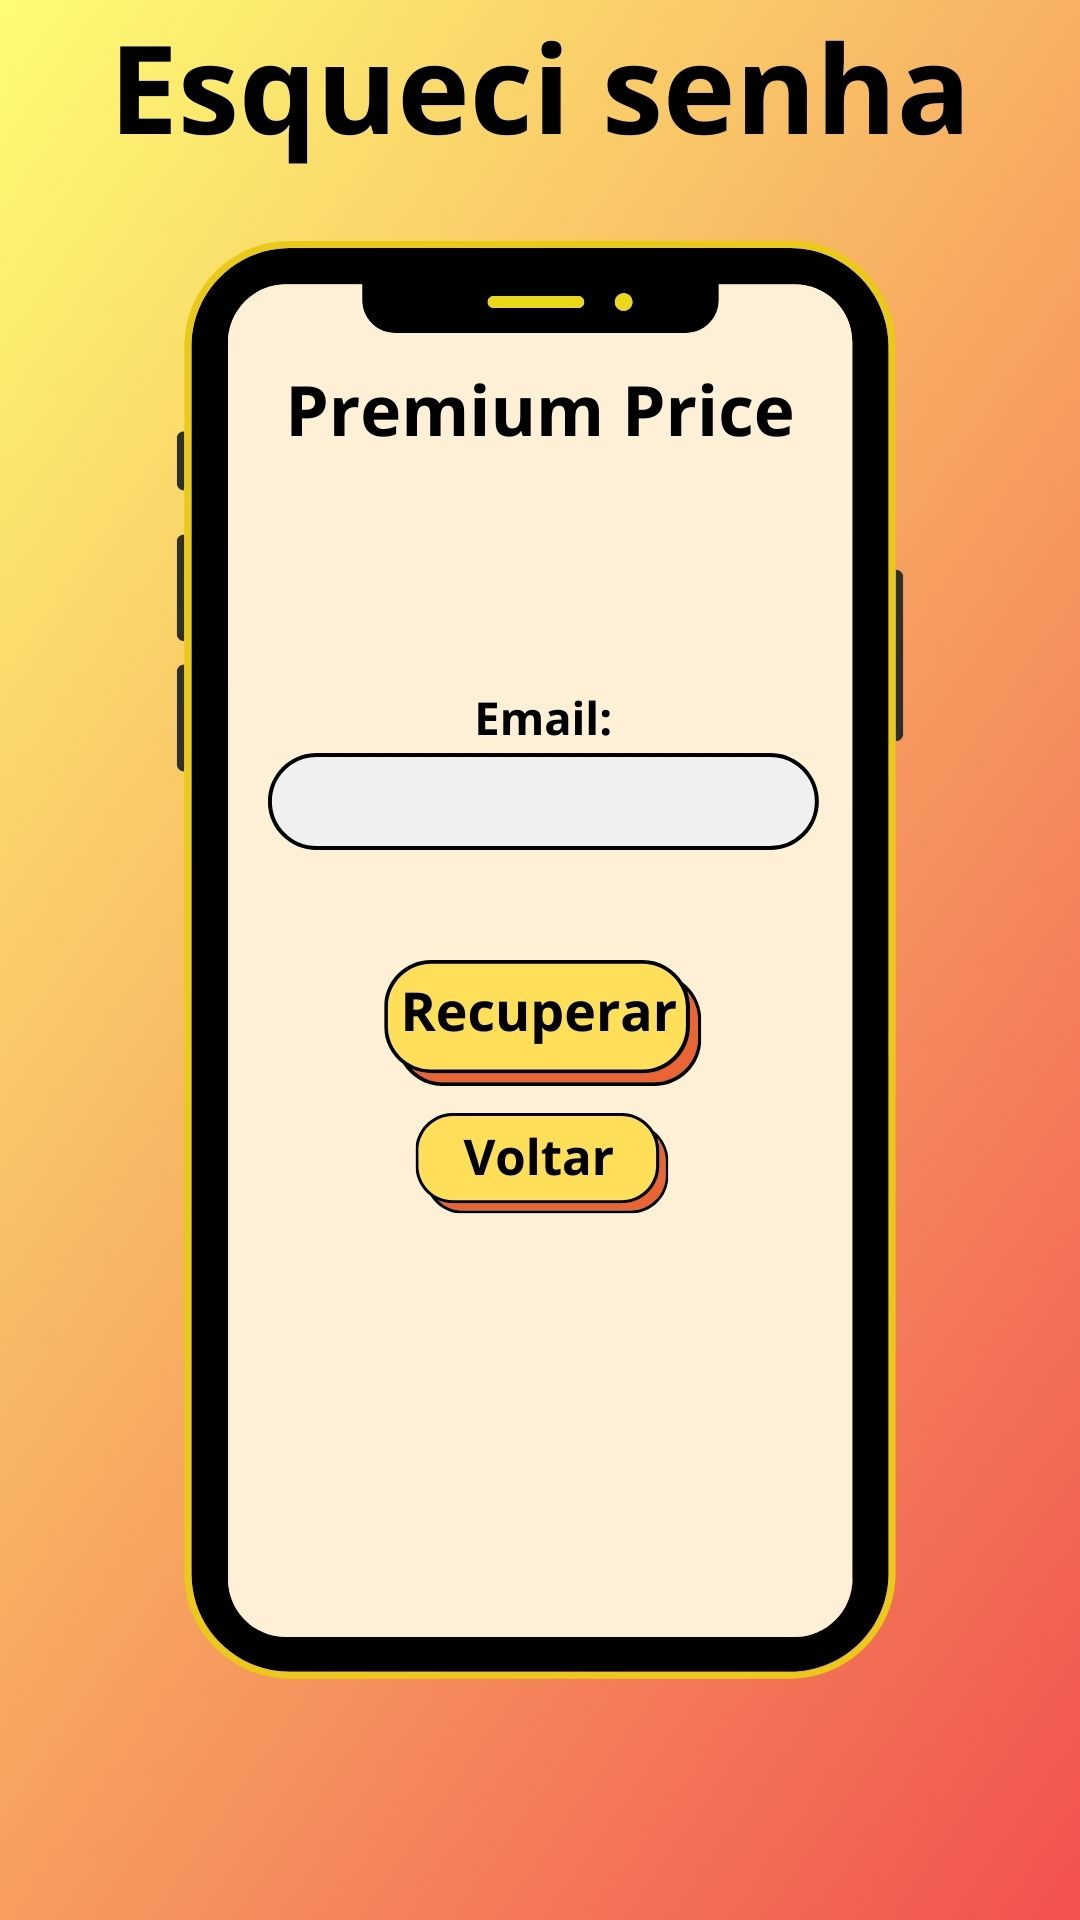
\includegraphics[width=\textwidth]{fig/telas/t_esqueci.jpg}
\footnotesize \centering
\par FONTE: O Autor (2024)
\end{figure}
\end{minipage}
 \\ \hline
\end{tabular}

\subsection*{\textbf{CRITÉRIOS DE ACEITAÇÃO}}

\begin{enumerate}[leftmargin=2cm]
    \item Deve permitir inserir email.
    \item Deve enviar nova senha gerada aleatoriamente para o email cadastrado.
\end{enumerate}

\subsection*{\textbf{CRITÉRIOS DE ACEITAÇÃO - DETALHAMENTO}}
\textbf{Critério de contexto} (Válido como premissa para todos os critérios):

\begin{tabularx}{0.9\textwidth}{@{}l X }
\textbf{Dado que} & Usuário clicou no botão "Esqueci minha senha". \\ 
\end{tabularx}


\begin{tabularx}{0.9\textwidth}{|l|X|}
\multicolumn{2}{@{}l}{\textbf{1. Deve permitir inserir email.}} \\ \hline
\textbf{Dado que} & Usuário está na tela de recuperação. \\ \hline
\textbf{Quanto} & Usuário clica no campo "Email". \\ \hline
\textbf{Então} & Sistema permite inserir email. \\ \hline
\end{tabularx}

\begin{tabularx}{0.9\textwidth}{|l|X|}
\multicolumn{2}{@{}l}{\textbf{\makecell[l]{2. Deve enviar nova senha gerada aleatoriamente para o email \\cadastrado.}}} \\ \hline
\textbf{Dado que} & Usuário preencheu corretamente. (R1) (R2) \\ \hline
\textbf{Quanto} & Usuário clica em "Recuperar". \\ \hline
\textbf{Então} & Sistema envia email com nova senha aleatória. \\ \hline
\end{tabularx}

\subsection*{\textbf{REGRAS DE NEGÓCIO DA HISTÓRIA}}

\begin{itemize}
    \item[] R1 - Email válido.
    \item[] R2 - Usuário cadastrado.
\end{itemize}


% Diagrama de Classes
% ----------------------------------------------------------
\chapter{Diagrama de Classes} \label{cha:diagramaclasses}

O diagrama de classes apresentado neste capítulo oferece uma representação visual das entidades e relacionamentos fundamentais que compõem a estrutura do aplicativo. Cada classe no diagrama representa um tipo de objeto no sistema, como produtos, localizações e usuários. Os atributos de cada classe são detalhados, fornecendo informações sobre as características e comportamentos dos objetos representados. 

Além disso, as associações entre as classes indicam as interações entre os objetos, como a relação entre produtos e localizações, usuários e produtos favoritos. O diagrama de classes é uma ferramenta valiosa para entender a estrutura e o funcionamento interno do aplicativo, auxiliando no desenvolvimento, manutenção e evolução do sistema ao longo do tempo.



%DUVIDA: explicação pro diagram?

\imagem{DIAGRAMA DE CLASSES}{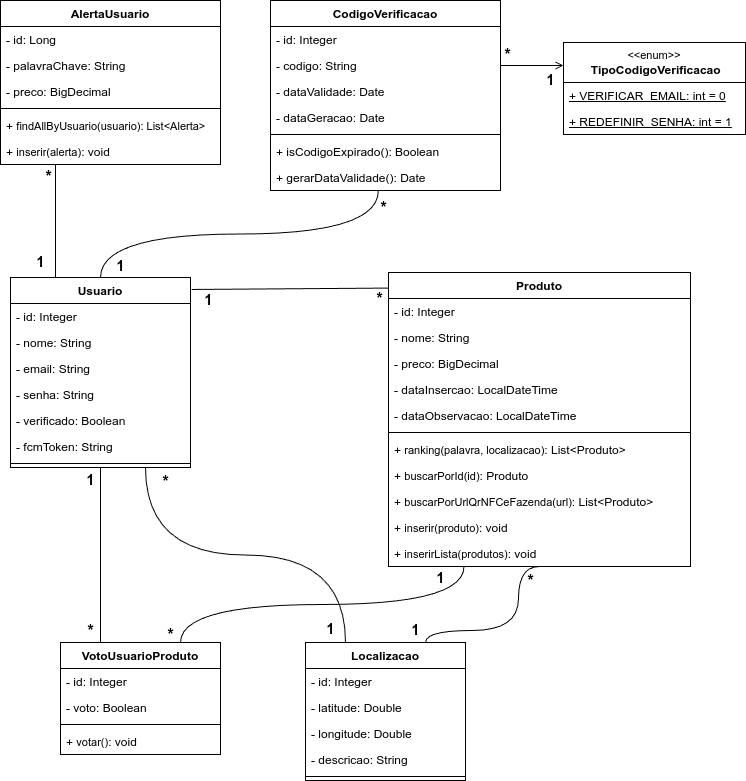
\includegraphics[width = 170mm]{fig/class.png}}{O Autor (2024)}{class}{nota(s)}{legenda(s)}

% Diagramas de Sequência
% ----------------------------------------------------------
\chapter{Diagramas de Sequência} \label{cha:diagramassequencia}

%Neste capítulo é apresentado o diagrama de classes.

%DUVIDA: explicação pro diagram?
%DUVIDA: precisa de todos os casos de uso,? sendo que alguns ja tao dentro um do outro

\section{Buscar produto}
\begin{figure}[H]
    \caption{\label{fig:label} DIAGRAMA DE SEQUÊNCIA BUSCAR PRODUTO}
    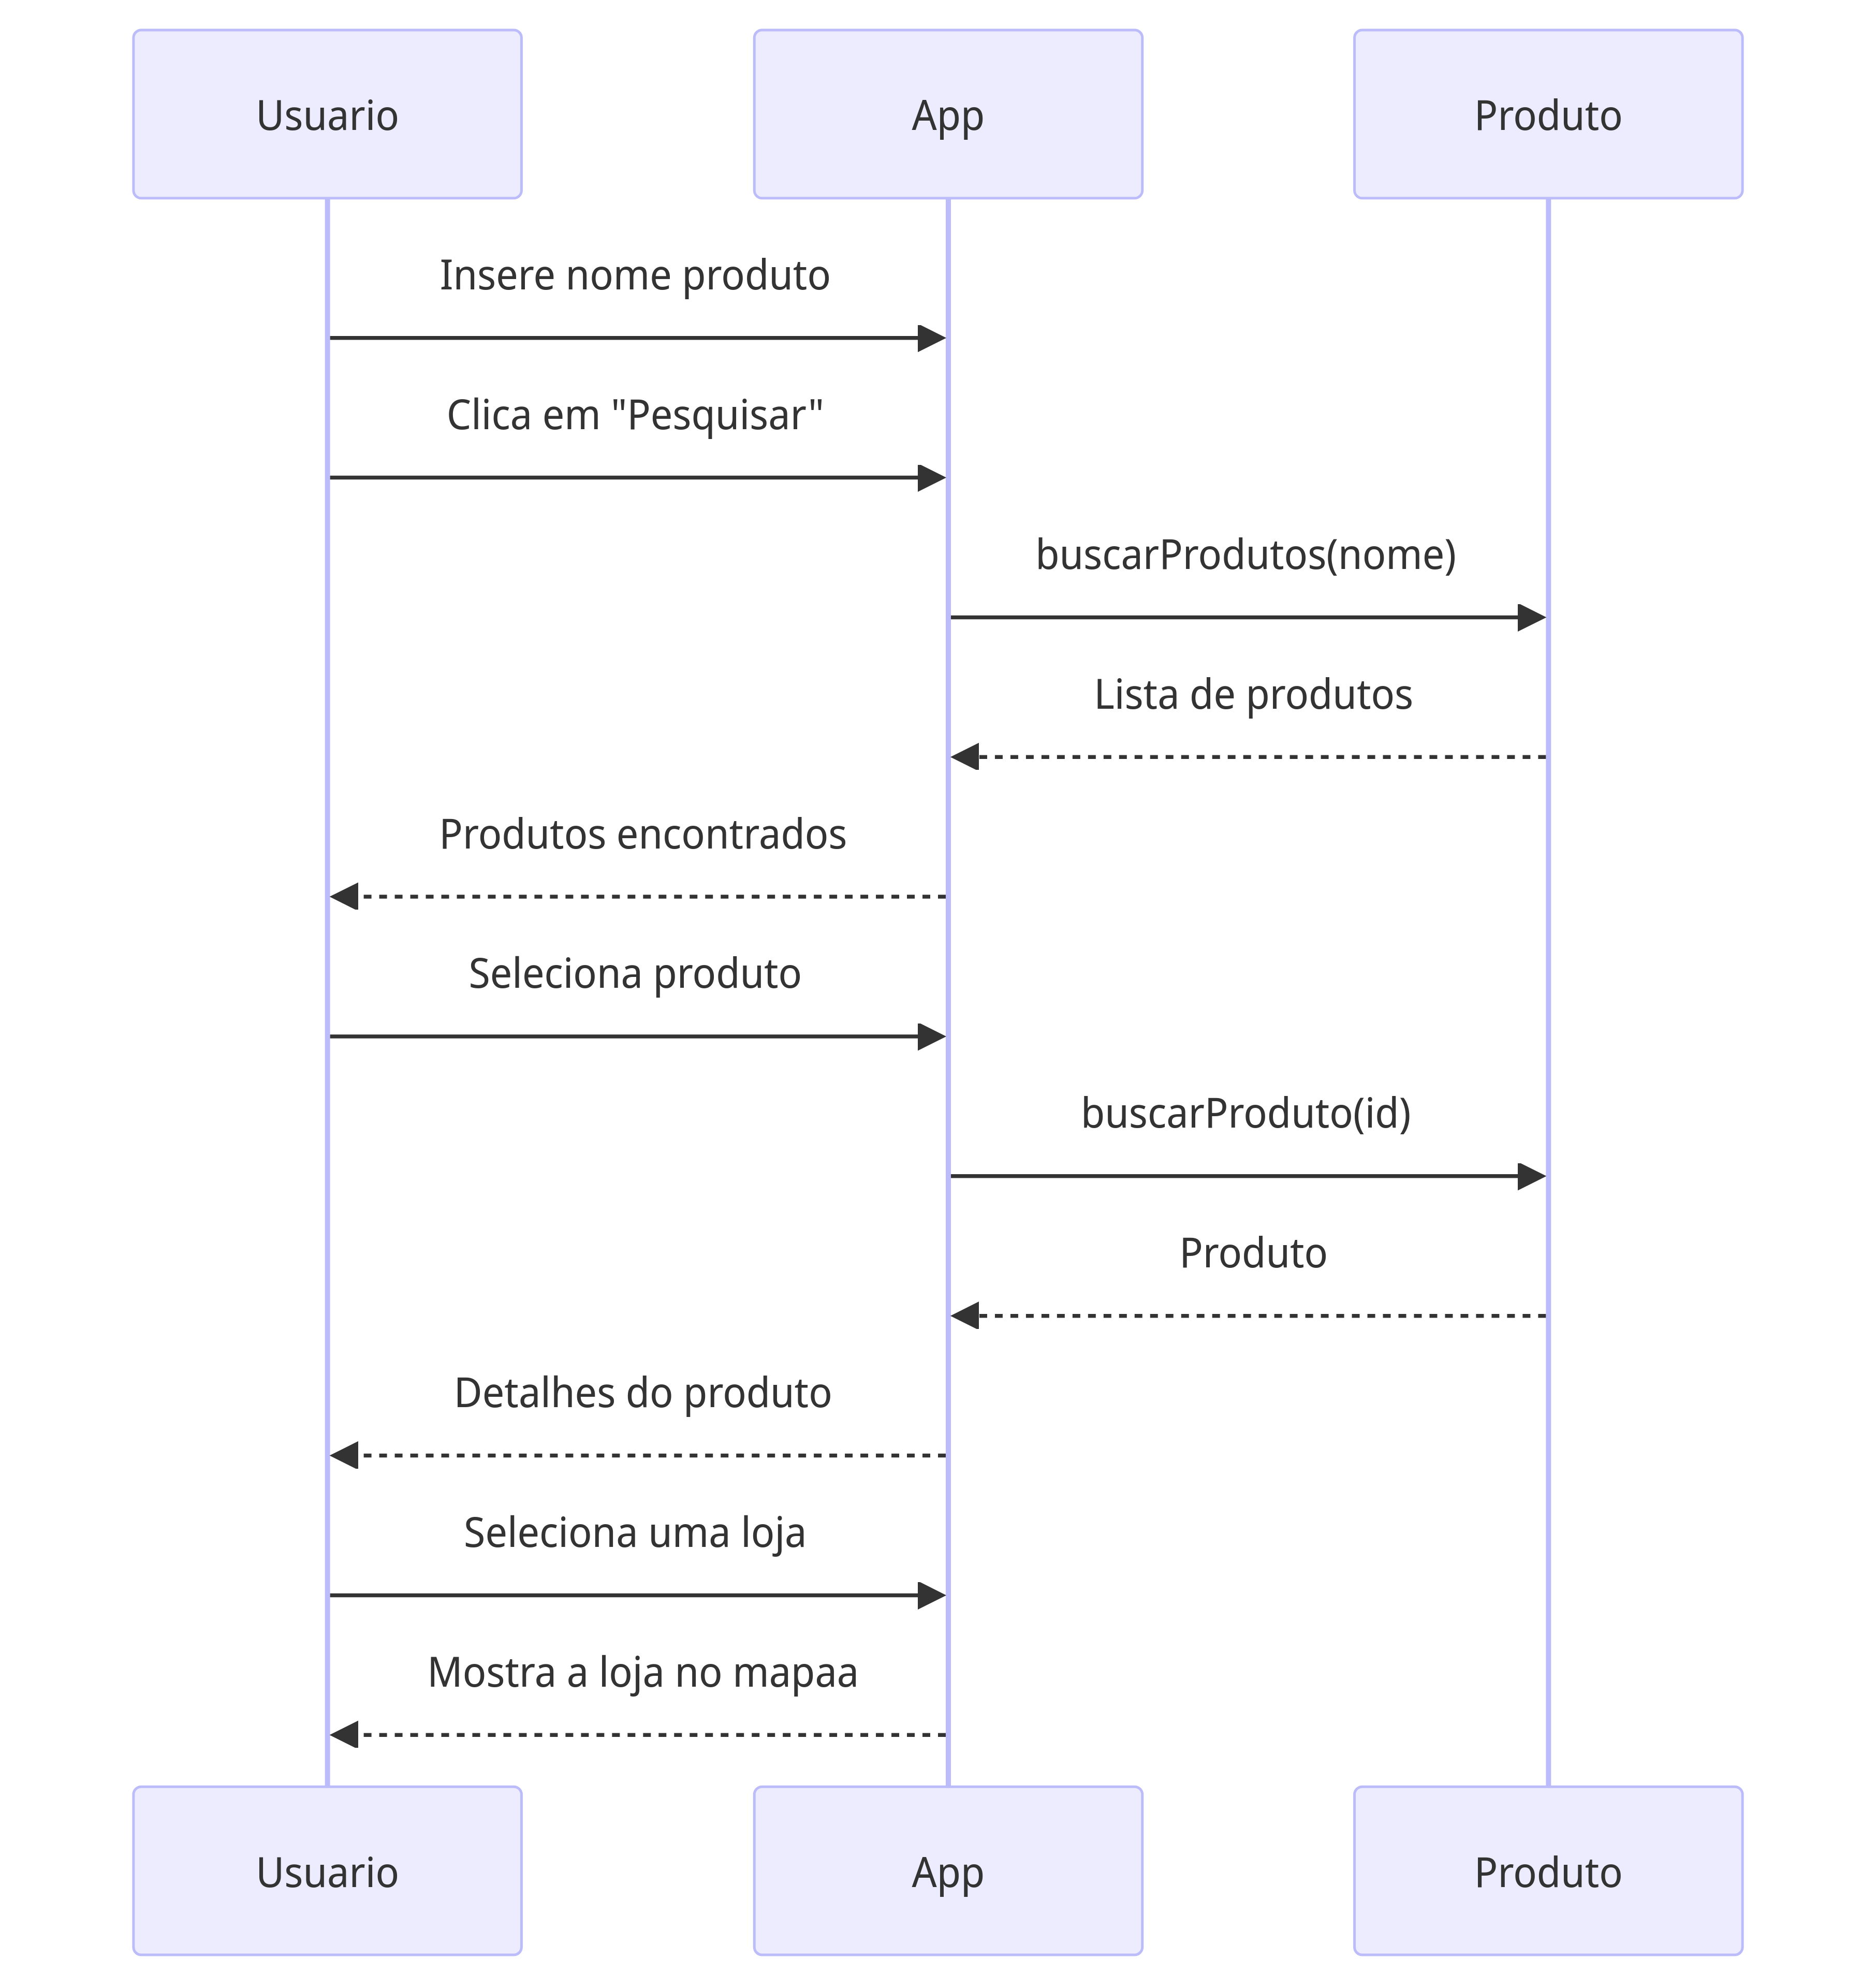
\includegraphics[width = 150mm]{fig/sequencia/sequencia1.png}
    \footnotesize \centering
    \par FONTE: O Autor (2024)
\end{figure}

\section{Avaliar sugestão}
\begin{figure}[H]
    \caption{\label{fig:label} DIAGRAMA DE SEQUÊNCIA AVALIAR SUGESTAO}
    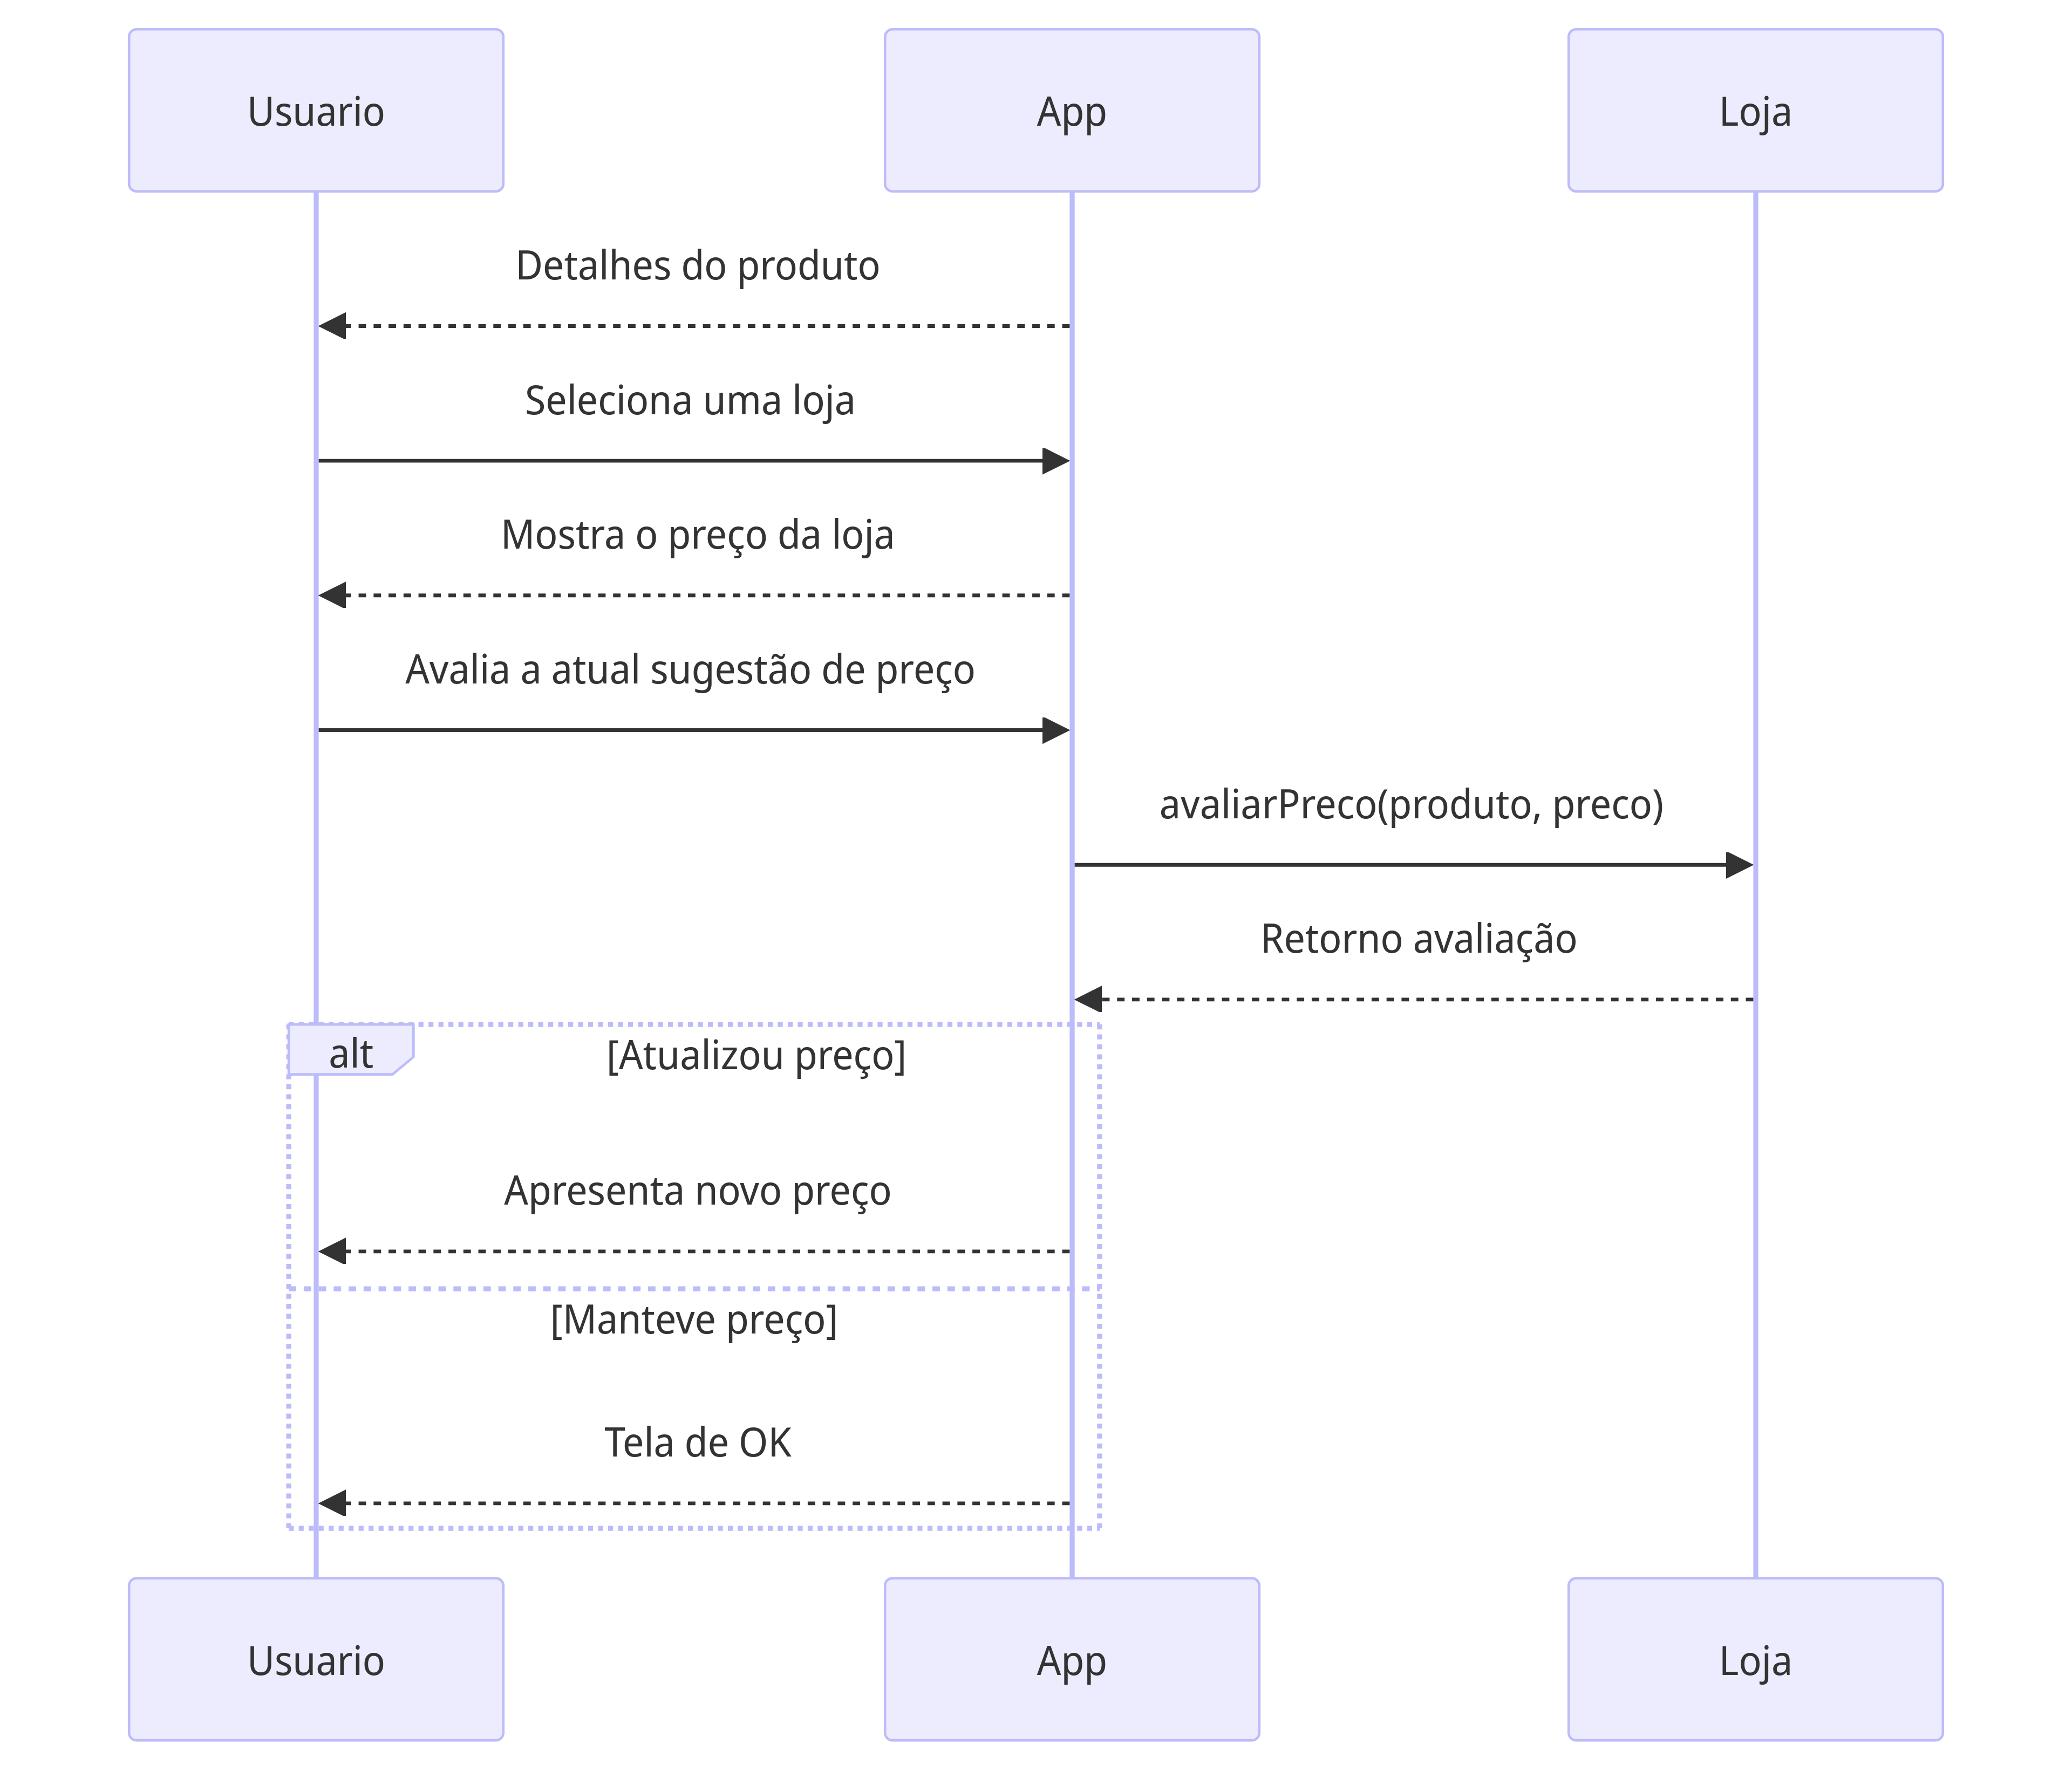
\includegraphics[width = 150mm]{fig/sequencia/sequencia2.png}
    \footnotesize \centering
    \par FONTE: O Autor (2024)
\end{figure}


\section{Sugerir edição}
\begin{figure}[H]
    \caption{\label{fig:label} DIAGRAMA DE SEQUÊNCIA SUGERIR EDIÇÃO}
    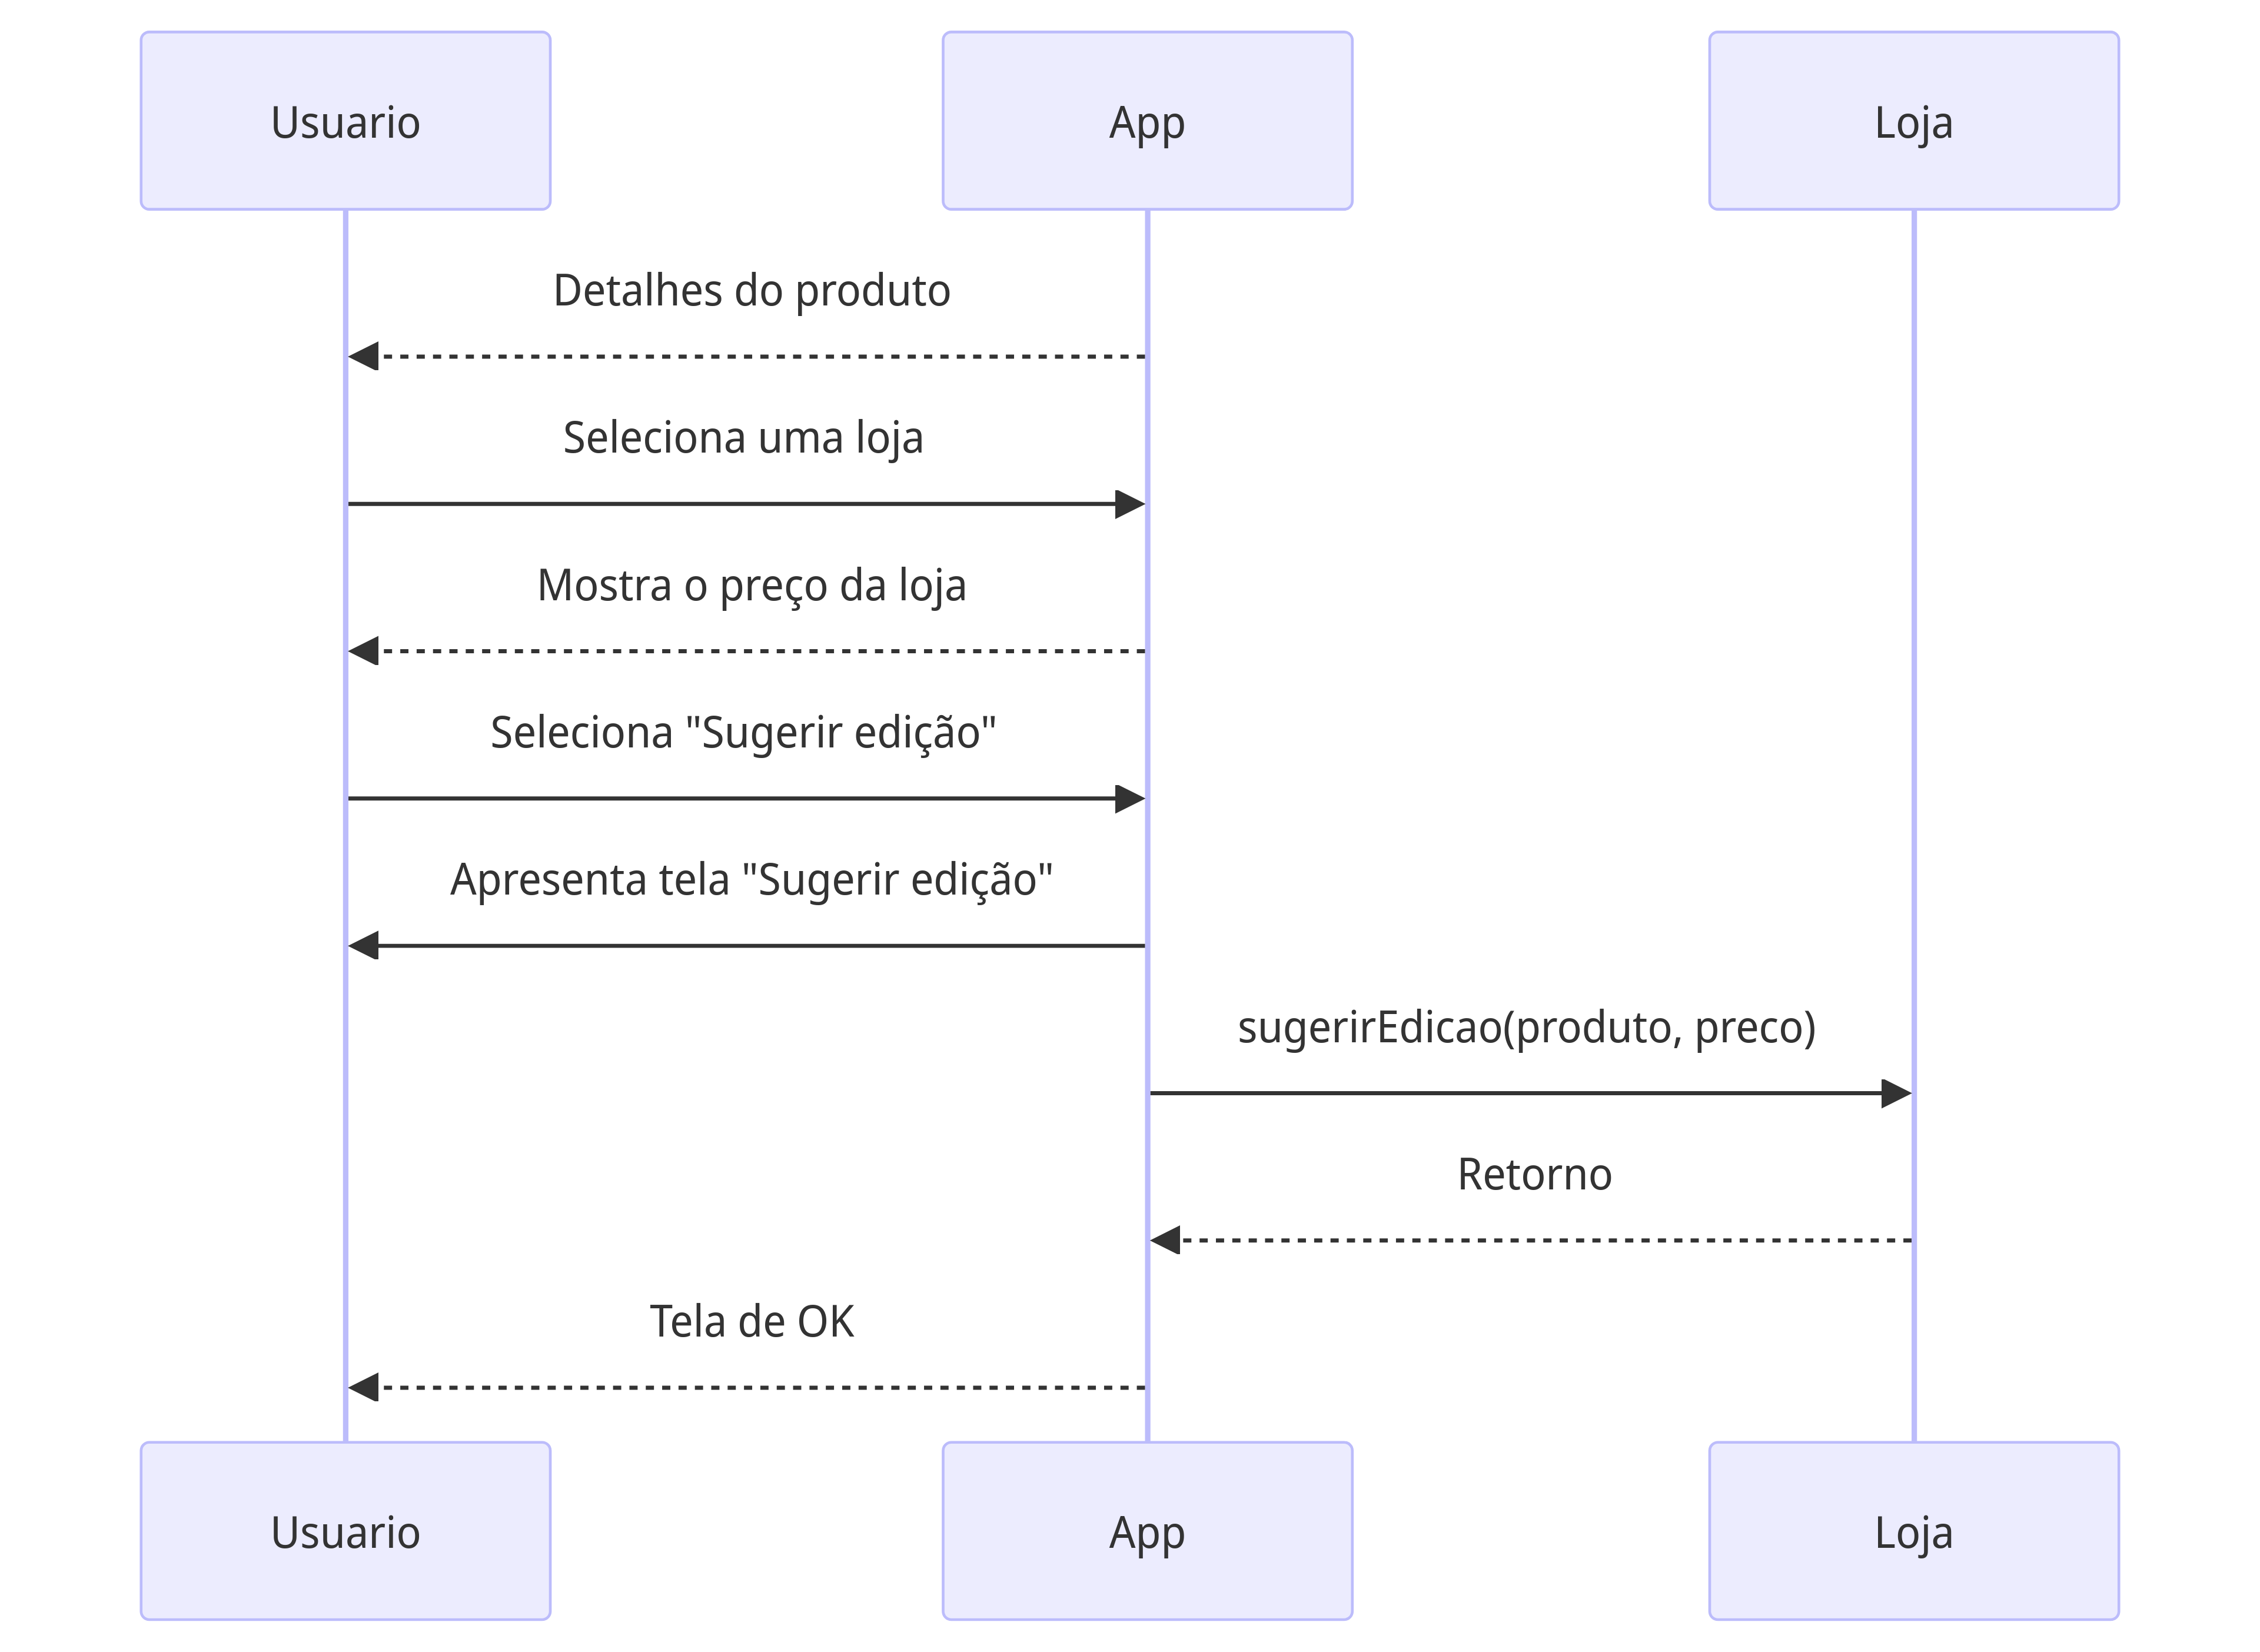
\includegraphics[width = 150mm]{fig/sequencia/sequencia3.png}
    \footnotesize \centering
    \par FONTE: O Autor (2024)
\end{figure}

\section{Cadastrar produto}
\begin{figure}[H]
    \caption{\label{fig:seqcadprod} DIAGRAMA DE SEQUÊNCIA CADASTRAR PRODUTO}
    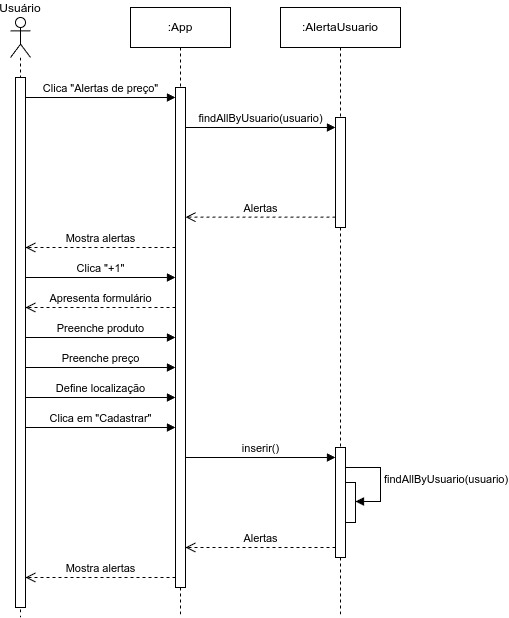
\includegraphics[width = 150mm]{fig/sequencia/sequencia4.png}
    \footnotesize \centering
    \par FONTE: O Autor (2024)
\end{figure}


%\section{Alterar senha}


%\section{Adicionar produto favorito}


%\section{Logar no sistema}


%\section{Criar conta}


%\section{Recuperar senha}

% Diagrama Físico do Banco de Dados
% ----------------------------------------------------------
\chapter{Diagrama Físico do Banco de Dados} \label{cha:diagramabanco}

Neste capítulo é apresentado o diagrama de classes.

\imagem{Diagrama Físico do Banco de Dados}{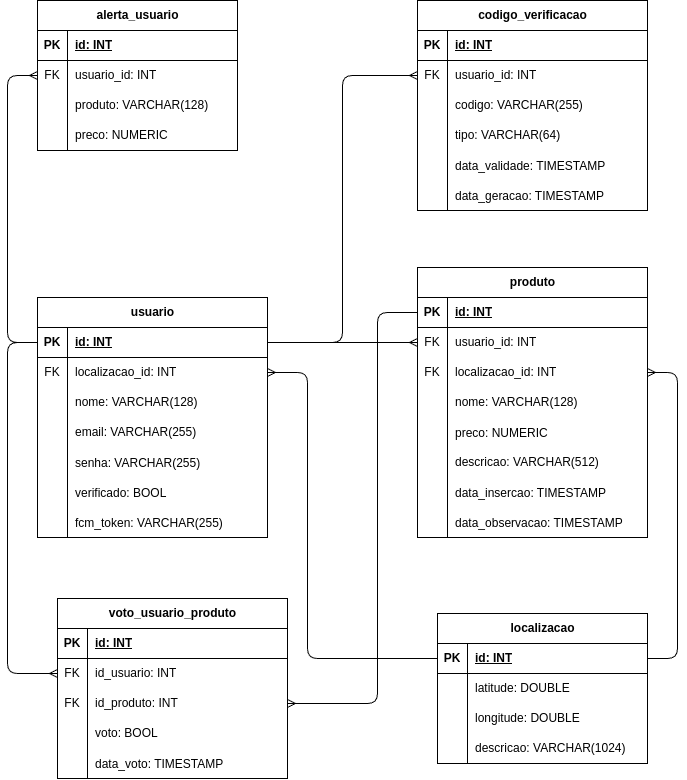
\includegraphics[width = 150mm]{fig/bd.drawio.png}}{O Autor (2024)}{bd}{nota(s)}{legenda(s)}

%\chapter{INTRODUÇÃO} \label{cha:introd}

Esta é uma série para apresentar o uso do template e não uma documentação da customização. Este documento pressume que você conheça algumas características de uso do LaTeX, caso não tenha nenhuma informação/formação, basta acessar o documento de documentação em pdf deste repositório. Nele você encontrará um curso básico de LaTeX para utilizar a customização sem muitas dificuldades.

Claro, a curva de aprendizado inicial é difícil de ser percorrida. Depois de se acostumar, fica mais simples e satisfatório.
\section{UTILIZAÇÃO DESTE TEMPLATE} \label{sec:util}

Veja que é necessário colocar os títulos do capítulo e da seção em caixa alta. É recomendado ter um texto entre as seções do documento.

Você pode digitar o texto e utilizar os recursos do LaTeX para colocar os elementos gráficos, tabelas, quadros, expressões matemáticas, siglas, símbolos, citações e referências. Foram configurados alguns comandos para facilitar o seu trabalho.
\subsection[Imagens]{Imagens e figuras}\label{ssec:imafig}

Para inserir uma figura com o comando \verb+\includegraphics+ para ficar de acordo com a normalização ABNT-UFPR:
\subsubsection{imagem}\label{sssec:imagem}

\verb+\imagem{Título da imagem}{largura}+ 

\verb+   {figura com sua localização }{Fonteda figura}+

\verb+   {label}{alguma nota}{alguma legenda}+

\begin{lstlisting}
\figura
{FIGURA DE TIPOS PARA IMPRESSAO}  % Titulo
{.75}                             % % da largura da linha
{fig/tipog.png}                   % caminho da figura
{\citefig{tipo2012}.}             % Fonte
{tipoex}                          % label = fig:tipoex
{Esta eh uma nota musical, 
 Esta eh uma nota musical e 
 Esta eh uma outra nota}          % Texto da Nota
{Nao quero colocar legenda.}      % Texto da Legenda
\end{lstlisting}

Para fazer referencia a esta figura, basta digitar \verb+\autoref{fig:tipoex}+.

Para inserir um elemento gráfico gerado/compativel com o LaTeX, você tem o comando imagem com 7 parâmetros:

\begin{lstlisting}
% simplificacao para colocar figuras
% ----------------------------------------------------------
%   Parametros
%    1 caption
%    2 percent textwidth
%    3 arquivo da figura
%    4 fonte
%    5 fig:label
%    6 nota
%    7 legenda

\figura
{FIGURA DE TIPOS PARA IMPRESSAO}  % Titulo
{.750}                            % %da largura da linha
{fig/tipog.png}                   % caminho da figura
{\citefig{tipo2012}.}             % Fonte
{tipoex}                          % label = fig:tipoex
{Esta eh uma nota musical. 
 Esta eh uma nota musical.
 Esta eh uma nota musical. 
 Esta eh uma nota e esta 
	eh uma outra nota}            % Texto da Nota
{Nao quero colocar legenda.}      % Texto da Legenda
\end{lstlisting}

Para fazer referência a esta figura, basta digitar \verb+\autoref{fig:tipoex}+

\begin{lstlisting}
% simplificacao para colocar imagens
% ----------------------------------------------------------
%   Parametros
%    1 caption
%    2 imagem tikz ou pgfplots ou outro elemento qualquer
%    3 fonte
%    4 fig:label
%    5 nota
%    6 legenda
\end{lstlisting}

\verb+\imagem{Titulo}{arg2}{fonte}{label}{nota(s)}{legenda(s)}+

\begin{lstlisting}
\imagem{Titulo}
	{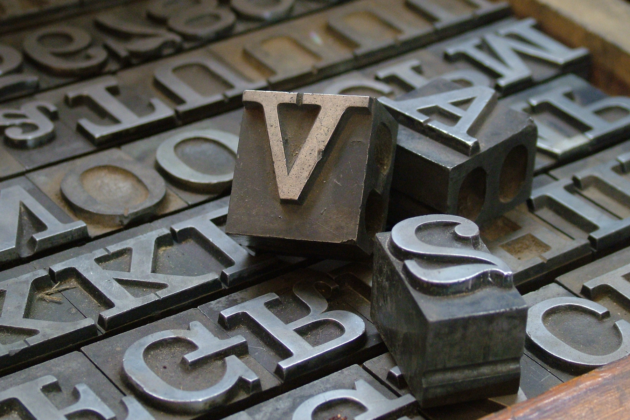
\includegraphics[width = 80mm]{fig/tipog}}
	{fonte}
	{label}
	{nota(s)}
	{legenda(s)}
\end{lstlisting}


\imagem{Titulo}{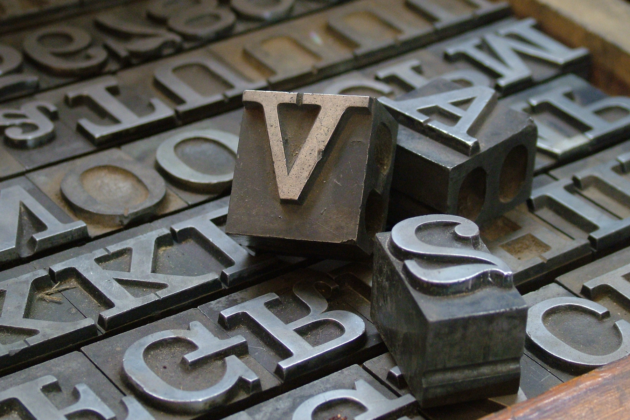
\includegraphics[width = 80mm]{fig/tipog}}{fonte}{label}{nota(s)}{legenda(s)}

Para fazer referência a esta figura é da mesma forma,\verb+\autoref{fig:label}+, \autoref{fig:label}

\subsection[Quadros e tabelas]{Quadros e tabelas}

Lembrando que quadros tem informações e são fechados lateralmente e verticalmente, tem a posição do título, fonte, nota e legenda diferentes da tabela.
\subsection[Quadros]{Inserir quadros}\label{ssec:quadros}

Para inserir um quadro são necessários 6 parâmetros:

\begin{lstlisting}
% ----------------------------------------------------------
%   Parametros
%    1 caption
%    2 elementos tabulados
%    3 fonte
%    4 qua:label
%    5 nota
%    6 legenda
\end{lstlisting}

Os elemento tabulados foram inseridos no ambiente tabular, com as laterais e parte superior e inferior fechados.

Este ambiente não quebra sua estrutura em páginas.

\begin{lstlisting}
\qquadro{Prefixos convencionados para referencias}
{\footnotesize
 \begin{tabular}{|l*{6}{|c}|}\hline
  \textbf{Elementos}:& 
       capitulos & secoes & 
       subsecoes & subsubsecoes &
       figuras   & imagens \\\hline
  \textbf{prefixos}:&
     cap &sec &
     ssec &sssec &
     fig & img\\\hline\hline
  \textbf{Elementos}:& tabelas &
     quadros & equacoes & exemplos &
     exercicios & questoes\\\hline	
  \textbf{prefixos}:&
     tab &    qua & 
     eq  &    exm & 
     exc &     que\\\hline\hline
  \textbf{Elementos}:& itens enumerados &
                       alineas&teoremas &
                       axiomas          & 
                       listagem         &\\\hline
  \textbf{prefixos}:&  inum & ali & teo & axi & lst &\\\hline
\end{tabular}}
{O autor(2021)}{quadrinho}{}{}
\end{lstlisting}

\qquadro{Prefixos convencionados para referencias}
{\footnotesize
 \begin{tabular}{|l*{6}{|c}|}\hline
  \textbf{Elementos}:& capítulos& 	seções&	subseções&	subsubseções&	
  figuras&	imagens \\\hline
  \textbf{prefixos}:&cap&sec&ssec&sssec&fig & img\\\hline\hline
  \textbf{Elementos}:&tabelas&	quadros&	
  equações& exemplos& exercícios & questões\\\hline	
  \textbf{prefixos}:&tab&qua&eq& exm & exc&que\\\hline\hline
  \textbf{Elementos}:&itens enumerados& alíneas&teoremas&	axiomas & listagem &\\\hline
  \textbf{prefixos}:&inum &ali&teo& axi &lst&\\\hline
\end{tabular}}
{O autor(2021)}{quadrinho}{}{}


A citação da fonte é feita por \verb+\citefig{bibkey}+.

Para fazer referência a este quadro, o comando \verb+\autoref{qua:quadrinho}+,\autoref{qua:quadrinho}


\subsection[Tabelas]{Inserir tabelas}

Para inserir uma tabela o comando é muito parecido, mas a normalização utilizada é o do IBGE na ABNT-UFPR.

\begin{lstlisting}
% simplificacao para colocar tabelas
% ----------------------------------------------------------
%   Parametros
%    1 caption
%    2 tabela
%    3 fonte
%    4 tab:label
%    5 nota
%    6 legenda


\tabela{T\'itulo do tabela}
{\begin{tabular}{r|c|c|c}\hline
		consumo & m\'edia & 
		m\'aximo & m\'inimo\\\hline
		& km/l& km/l& km/l\\\hline
		cidade & 11.5 & 14.8& 9.3 \\\hline
		estrada& 16.2 & 20.7& 13.4 \\\hline
\end{tabular}}
{\textcite{0230}}{exemplo}{Uma nota}{Uma legenda}
\end{lstlisting}


\tabela{T\'itulo do tabela}
{\begin{tabular}{r|c|c|c}\hline
		consumo & m\'edia & 
		m\'aximo & m\'inimo\\\hline
		& km/l& km/l& km/l\\\hline
		cidade & 11.5 & 14.8& 9.3 \\\hline
		estrada& 16.2 & 20.7& 13.4 \\\hline
\end{tabular}}
{\textcite{0230}}{exemplo}{Uma nota}{Uma legenda}


A citação da fonte é feita por \verb+\citefig{bibkey}+.

Para fazer referência a este quadro, o comando \verb+\autoref{tab:exemplo}+, \autoref{tab:exemplo}
\subsection[Equações]{Expressões matemáticas}

De preferencia ao uso do ambiente align:

\begin{lstlisting}
\begin{align}
 x + y &= 0\\
 x - y &= 2 \label{eq:2}
\end{align}
\end{lstlisting}


\begin{align}
x + y &= 0\\
x - y &= 2 \label{eq:2}
\end{align}

\subsection[Acronimos]{Siglas e símbolos}


\verb+\criarsimbolo{$\alpha$}{coeficiente de dilatação térmica}+ 

\criarsimbolo{$\alpha$}{coeficiente de dilatação térmica}, cria o símbolo e deixa anotado no texto;

\verb+\criarsigla{UFPR}{Universidade Federal do Paraná}+ 

\criarsigla{UFPR}{Universidade Federal do Paraná}\label{item:UFPR} apenas cria a sigla, sem deixar nada anotado no texto;

\verb+\criarsigla*{ABNT}{Associação Brasileira de Normas Técnicas}+ 

\criarsigla*{ABNT}{Associação Brasileira de Normas Técnicas} cria a sigla e deixa anotado no texto.

\subsection[Citações]{Citações e referências}

Para criar citações indiretas: Segundo \verb+\textcite{abntex2cite}+, \textcite{abntex2cite}.


Para citações diretas: "[...] tudo bem quando acaba bem."\cite{abntex2cite}. \verb+\cite{abntex2cite}+


\subsubsection{Criação de referencias citadas}

Para as citações feitas para serem empregadas no texto eu customizei a separação das referências bibliográficas através de \textit{keys}.


\subsubsection{Criação de referencias consultadas}

A criação de uma bibliografia consultada após o capítulo de referências do trabalho é feita para as referências que foram utilizadas com o \textit{key}= {consulta}:

\begin{lstlisting}
....
key={consultada},
....
\end{lstlisting}  


\subsubsection{Criação de referencias de documentos não publicados ou informais}

A criação de uma bibliografia consultada após o capítulo de referências do trabalho é feita para as referências que foram utilizadas com o \textit{key}= {npub-informal}:

\begin{lstlisting}
....
key={npub-informal},
....
\end{lstlisting}  

%%%%%%%%%%%%%%%%%%%%%%%%%%%%%%%%%%%%%%%%%%%%%%%%%%%%%%%%%%%%%%%%%

no arquivo referencias.bib, no manual ABNTeX2Modelo-glossario foi adicionado a key de consulta.

\begin{lstlisting}
@Manual{abntex2modelo-glossario,
	Title = {Exemplo de uso de gloss{\'a}rio com abnTeX2},
	Author      = {abnTeX2},
	Organization= {Equipe abnteX2},
	Year        = {2013},
	Bdsk-url-1  = {http://abntex2.googlecode.com/},
	Date-added  = {2013-03-11 13:38:46 +0000},
	Date-modified={2013-04-05 11:03:36 +0000},
	Url         = {http://abntex2.googlecode.com/},
	key         = {consulta},
}
\end{lstlisting}

adicionada a chave \textit{key}= = {consulta} para que ele seja mencionado na lista de obras consultadas.


\subsubsection{Para fazer referência às seções ou elementos enumerados}

\begin{lstlisting}
1. Capitulos: \verb+\autoref{cha:introd}+ 

2. Secoes: \verb+\autoref{sec:util}+ 

3. Subsecoes: \verb+\autoref{ssec:imafig}+

4. Imagens: \verb+\autoref{sssec:imagem}+ 

5. Apendices: \verb+\autoref{ap:primeiroAp}+ 
          
6. Anexos: \verb+\autoref{ax:primeiroAx}+ 
          
7. Equacoes: \verb+\autoref{eq:2}+

8. Itens enumerados \verb+\autoref{item:UFPR}+ 
	
\end{lstlisting}


% Finaliza a parte no bookmark do PDF
% para que se inicie o bookmark na raiz
% e adiciona espaço de parte no Sumário
% ----------------------------------------------------------
%\phantompart

% ---
% Conclusão (outro exemplo de capítulo sem numeração e presente no sumário)
% ---
%\chapter*[Conclusão]{Conclusão}
%\addcontentsline{toc}{chapter}{Conclusão}
% ---
%\input{cap06}

% ELEMENTOS PÓS-TEXTUAIS
% ----------------------------------------------------------
\postextual

% Ajuste vertical do titulo de referencias no sumário
% ----------------------------------------------------------
\addtocontents{toc}{\vspace{-6pt}}

% Referências bibliográficas
% ----------------------------------------------------------
%\bibliography{referencias}

\begingroup

\printbibliography[heading=bay,notkeyword= {consulta}, notkeyword={npub-informal}]

\printbibliography [keyword= consulta, title = FONTES DE CONSULTA]
\endgroup

% ----------------------------------------------------------

% Ajuste vertical dos titulos dos capitulos postextuais
% ----------------------------------------------------------
\addtocontents{toc}{\vspace{4pt}}

% Glossário
% ----------------------------------------------------------
% Consulte o manual da classe abntex2 para orientações sobre o glossário.
%
%\glossary

% Apêndices
% ----------------------------------------------------------
\ifthenelse{\equal{\terApendice}{Sim}}
{\begin{apendicesenv}

        % Numeração arábica para os apêndices
        % --------------------------------------------------
        \renewcommand{\thechapter}{\arabic{chapter}}
        % Imprime uma página indicando o início dos apêndices
        % \partapendices

        % Existem várias formas de se colocar anexos.
        % O exemplo abaixo coloca 2 apêndices denominados de 
        % DESENVOLVIMENTO DETALHADO DA PINTURA e 
        % ESCOLHA DO MATERIAL DE IMPRESSÃO:
        % ---
        % --- insere um capítulo que é tratado como um apêndice
        %\chapter{DESENVOLVIMENTO DETALHADO DA PINTURA}
        % 
        %\lipsum[29] % gera um parágrafo
        %
        % --- insere um capítulo que é tratado como um apêndice
        %\chapter{ESCOLHA DO MATERIAL DE IMPRESSÃO}
        % 
        %\lipsum[30] % gera um parágrafo

        % --- Insere o texto do arquivo ap01.tex
        % 
        % --- O conteúdo do arquivo pode ser vários anexos ou um único apêndices.
        %     A vantagem de se utilizar este procedimento é de suprimi-lo
        %     das compilações enquanto se processa o resto do documento.

           % --- insere um capítulo que é tratado como um apêndice
   \label{ap:ap01}
   \chapter{ESCOLHA DO MATERIAL - colocado no apendice}
    
   \lipsum[30] % gera um parágrafo
   \section*{Testes se\c{C}\~aO}

    \lipsum[22] % gera um parágrafo
	
	\chapter{ESCOLHA DO MATERIAL DE IMPRESSÃO- colocado no apendice}
    \lipsum[32] % gera um parágrafo


\end{apendicesenv}
}{}

% Anexos
% ----------------------------------------------------------
\ifthenelse{\equal{\terAnexo}{Sim}}{
\begin{anexosenv}

        % Numeração arábica para os apêndices
        % --------------------------------------------------
        \renewcommand{\thechapter}{\arabic{chapter}}
        % --- Imprime uma página indicando o início dos anexos
        % \partanexos

        % Existem várias formas de se colocar anexos.
        % O exemplo abaixo coloca 2 anexos denominados de 
        % TABELA DE VALORES e GRÁFICOS DE BALANCEMANTO:
        % ---
        % --- insere um capítulo que é tratado como um anexo
        %\chapter{TABELAS DE VALORES}
        % 
        %\lipsum[31] % gera um parágrafo
        %
        % --- insere um capítulo que é tratado como um anexo
        %\chapter{GRÁFICOS DE BALANCEAMENTO}
        % 
        %\lipsum[32] % gera um parágrafo

        % --- Insere o texto do arquivo ax01.tex
        % 
        % --- O conteúdo do arquivo pode ser vários anexos ou um único anexo.
        %     A vantagem de se utilizar este procedimento é de suprimi-lo
        %     das compilações enquanto se processa o resto do documento.

            % --- insere um capítulo que é tratado como um apêndice
   \chapter{anexando ESCOLHA DO MATERIAL}
    
   \lipsum[30] % gera um parágrafo
    \section*{anexando testes secao}
    

\chapter{anexando ESCOLHA DO MATERIAL DE IMPRESSÃO}
    
   \lipsum[32] % gera um parágrafo
 
\end{anexosenv}
}{}

% INDICE REMISSIVO
%---------------------------------------------------------------------
\ifthenelse{\equal{\terIndiceR}{Sim}}{
\phantompart
\printindex
}{}

\end{document}
